We perform the analysis on a dataset corresponding to \intlumi\ integrated luminosity. 
In this section we document the results obtained after the $\zz$ preselection defined in 
Section~\ref{sec:selection} and the final mass-dependent $\hzz$ selections using cut-based approach. 

\subsection{Results after looser selections}

We compare the data with simulation in looser selections than the signal region 
to verfity the agreement in the key kinematic observables that we select on. 

Figure~\ref{fig:npv} shows the number of primary vertices in $ee$ and $\mu\mu$ final states 
after the $\ZZ$ preselections, comparing data to the simulation which was reweighted in the 
number of pile up events to match the values in data. This is a validation of the reweighting procedure. 
Figures~\ref{fig:zmass_zzpresel_mm}-\ref{fig:zmass_zzpresel_ee} show the dilepton mass distributions 
after applying all $\ZZ$ preselections except for the dilepton mass cuts, comparing data 
with simulation for the $\mu\mu$ amd $ee$ final states respectively in different jet 
bin final states. We observe in general a good agreement, except for a slight shift in the 
$\mu\mu$ final states. Figures~\ref{fig:zpt_zzpresel_mm} and~\ref{fig:zpt_zzpresel_ee} 
show the dilepton $p_T$ spectrum after the $\ZZ$ preselections for $\mu\mu$ and $ee$ final states. 
This provides an initial validation of the $\dyll$ background estimation. 

Table~\ref{tab:zzselection_all_2fb} shows the number of events observed in
data, comparing to the expected background contribution at the \zz
preselection level. The background estimation was discussed at Section~\ref{sec:backgrounds}. 
We validate the observables that are used in the higgs signal extraction at the 
$\ZZ$ preselection level. 
Figures~\ref{fig:met_zzpresel_mm}-\ref{fig:dphijetmet_zzpresel_ee} show 
the data to simulation comparions of the $\met$, $m_T$ and $\Delta\phi(jet,met)$ distributions. 
Good agreement between data and simulation is observed. 

%%%%%%%%%%%%%%%%%%
\begin{table}[!ht]
\begin{center}
\begin{tabular}{c|c|c|c}
\hline
sample 	& mm 	& ee 	 & TOTAL\\ \hline 
WW/Top	& 104.58 $\pm$ 7.83	& 77.95 $\pm$ 5.83	& 182.53 $\pm$ 9.77 \\ 
ZZ	& 48.43 $\pm$ 0.20	& 33.91 $\pm$ 0.17	& 82.34 $\pm$ 0.26 \\
WZ	& 33.74 $\pm$ 0.26	& 24.34 $\pm$ 0.23	& 58.07 $\pm$ 0.35 \\
Zjets	& 405.78 $\pm$ 12.62	& 287.59 $\pm$ 8.62	& 693.37 $\pm$ 15.28 \\ 
\hline
Total Background	& 592.53 $\pm$ 14.86	& 423.78 $\pm$ 10.42	& 1016.31 $\pm$ 18.14 \\ \hline 
DATA	& 572 	& 478	& 1050 \\ \hline 
\end{tabular}
\caption{Expected number of signal and background events corresponding to an 
integrated luminosity of \intlumi after applying the \zz preselections. 
Only statistical uncertaities are reported. The $\Wjets$ background is neglible thus omitted in the table.
%The background predictions do not have the data-to-simulation scale factors applied. 
}
\label{tab:zzselection_all_2fb}
\end{center}
\end{table}
%%%%%%%%%%%%%%%%%%

%%%%%%%%
\begin{figure}[!hbtp]
\begin{center}
\subfigure[Inclusive]{\label{subfig:npv_mm}
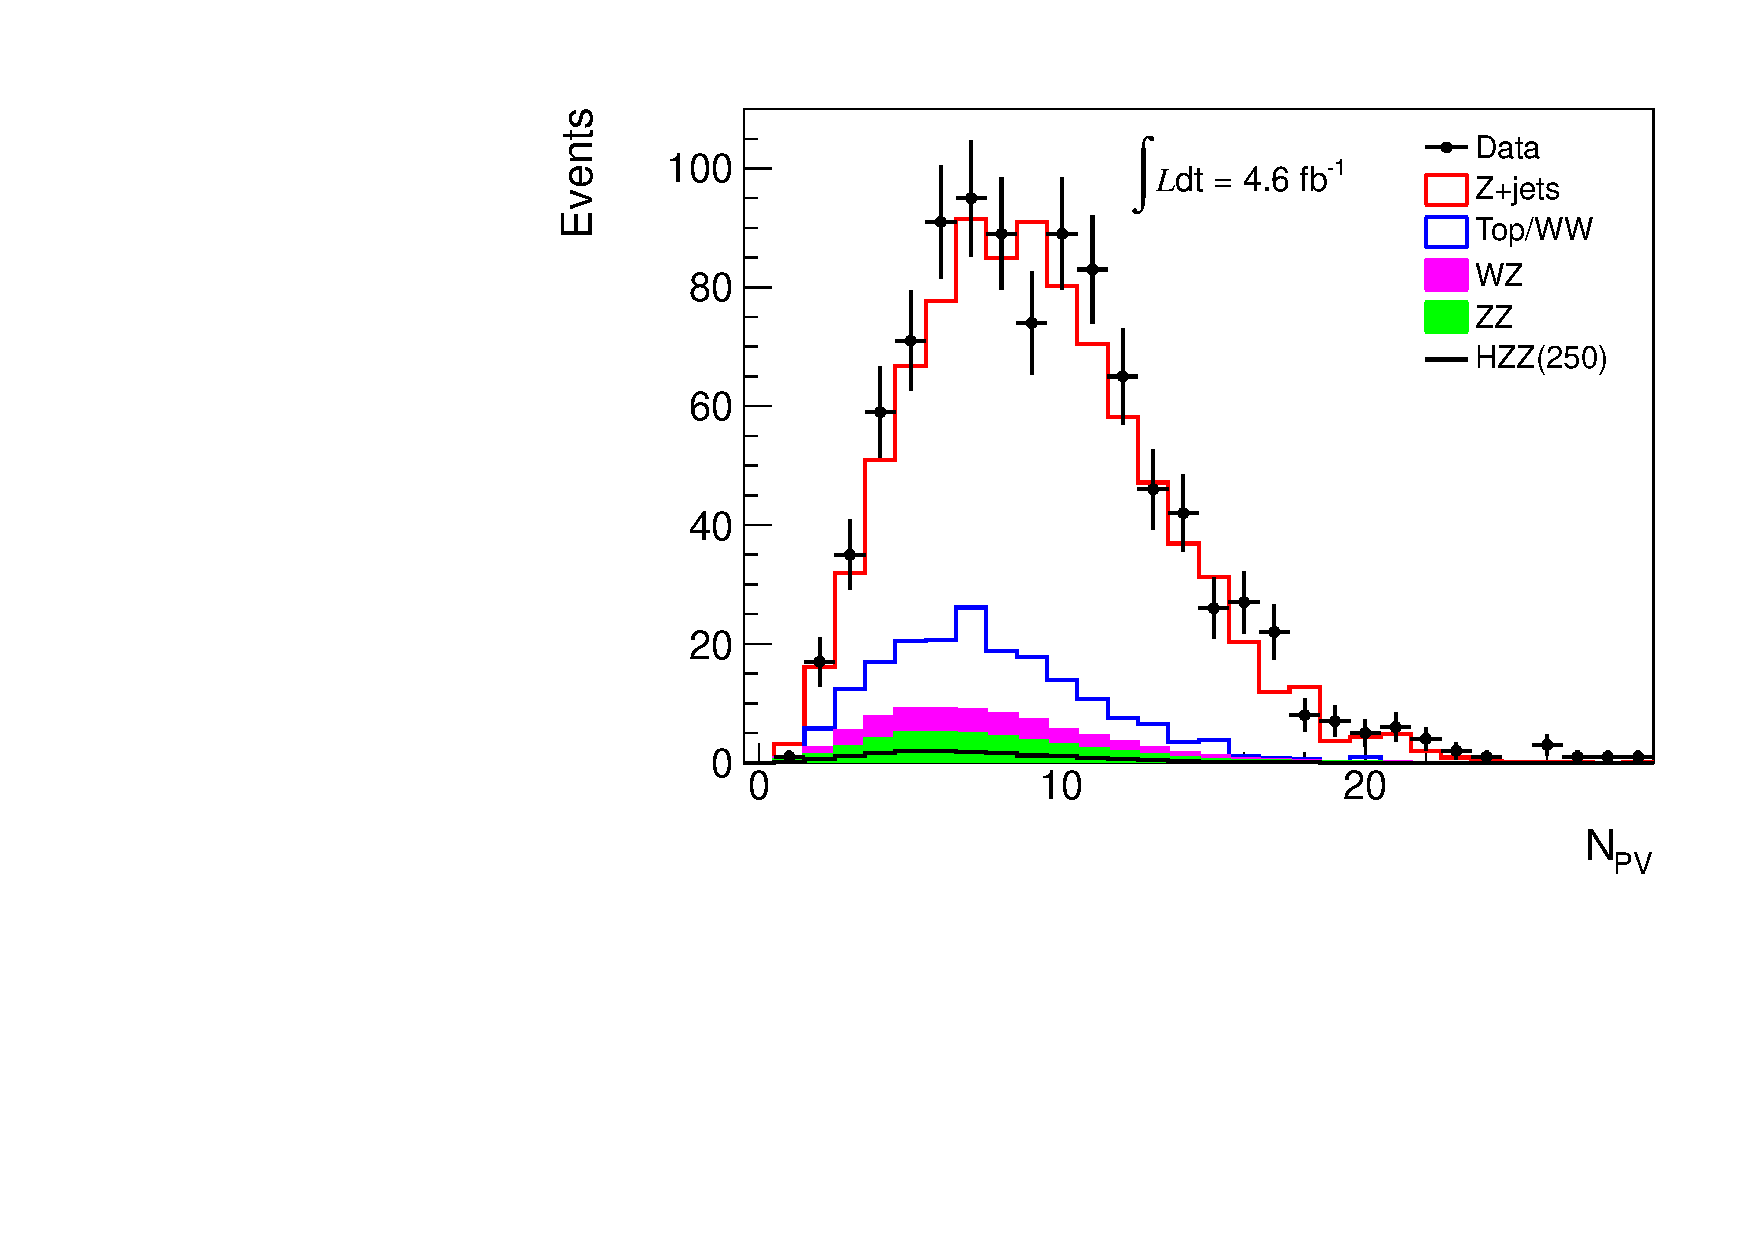
\includegraphics[width=.4\textwidth]{figures/presel_mH250_ee_npv.pdf}}
\subfigure[1-Jet]{\label{subfig:npv_ee}
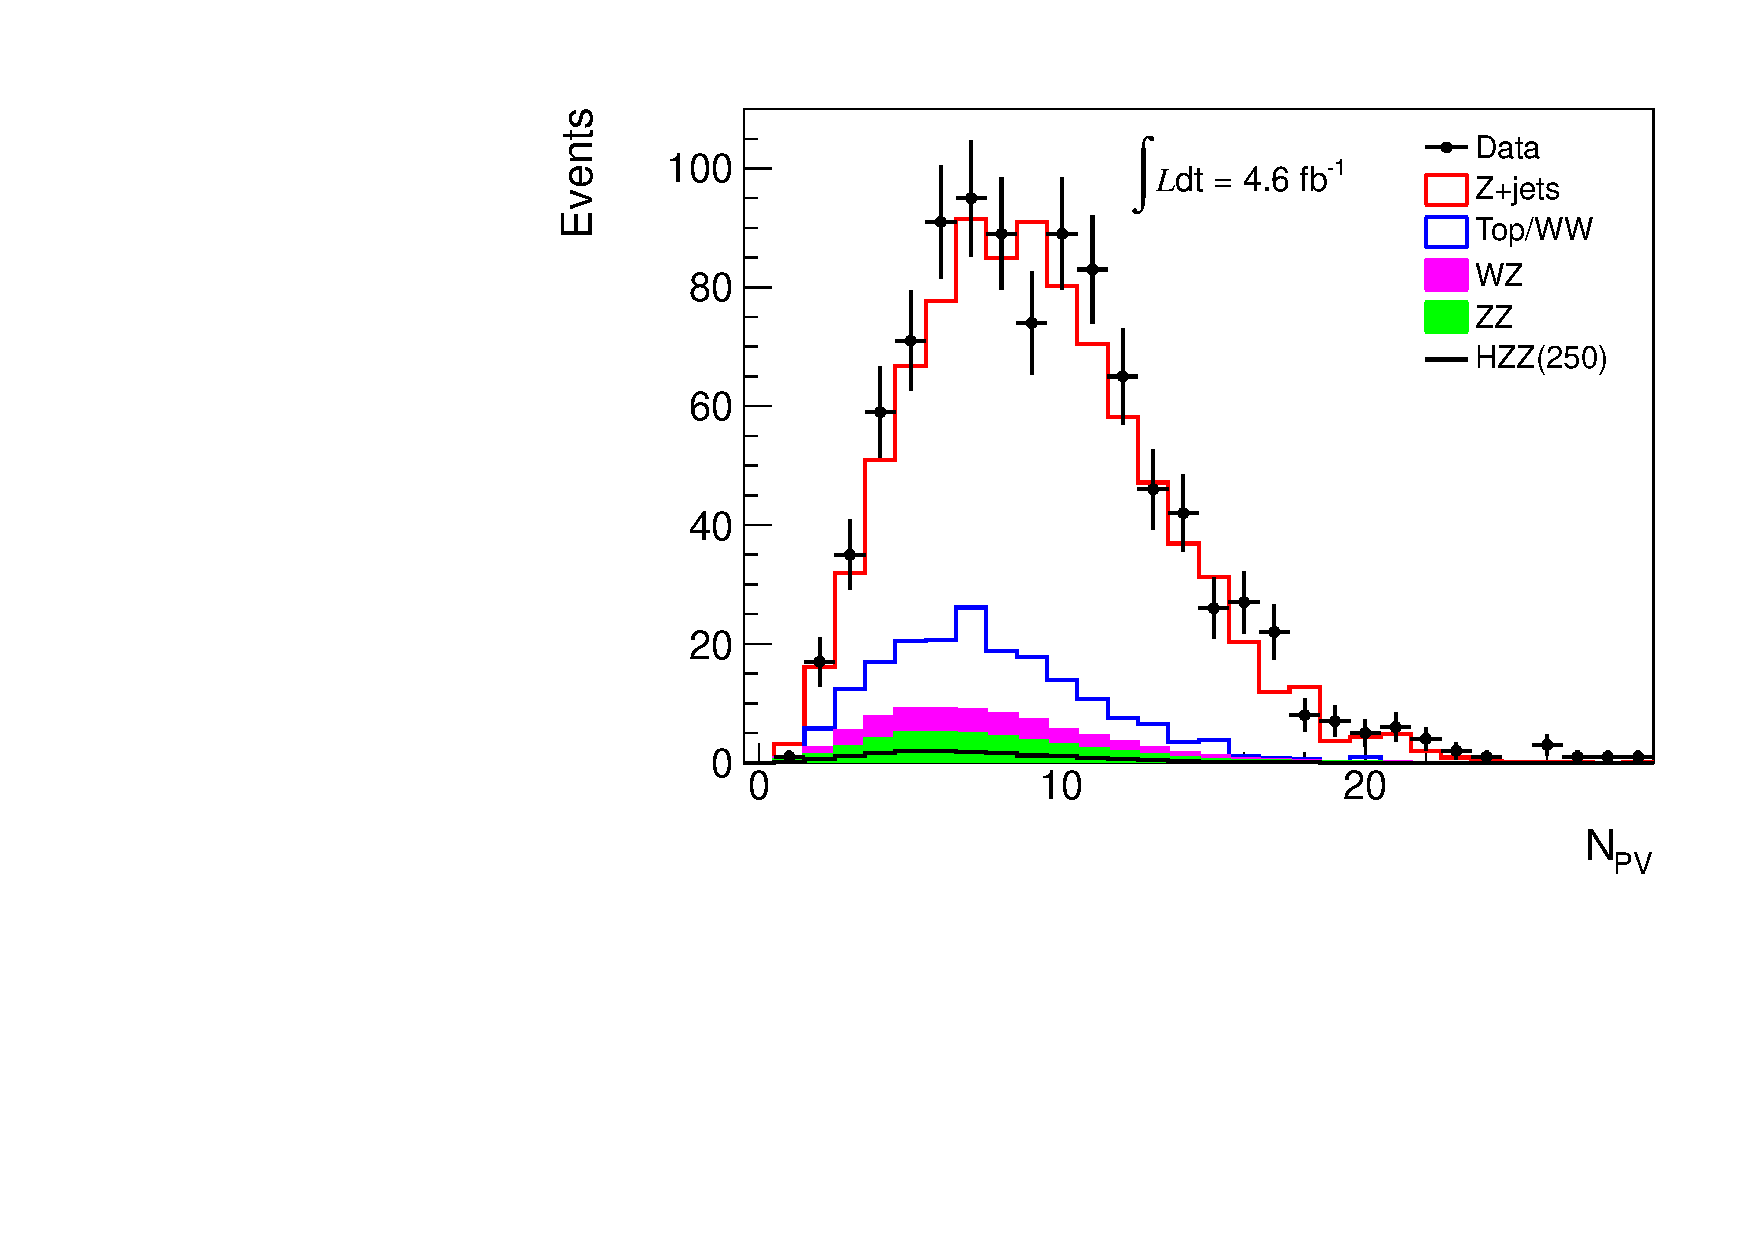
\includegraphics[width=.4\textwidth]{figures/presel_mH250_ee_npv.pdf}}
\caption{Distribution for the number of reconstructed primary vertices after the $\ZZ$ preselection observed in data corresponding 
to $2.1$~\ifb data in the muon~\subref{subfig:npv_mm} and electron~\subref{subfig:npv_ee} channels, compared to the expected from simulation for signal 
and background. The MC backgrounds are scaled as appropriate and the photon+jets estimate of the Z+jets background is added to the stack.}
\label{fig:npv}
\end{center}
\end{figure}
%%%%%%%%

%%%%%%%%
\begin{figure}[!hbtp]
\begin{center}
\subfigure[Inclusive]{\label{subfig:zmass_mm_incl}
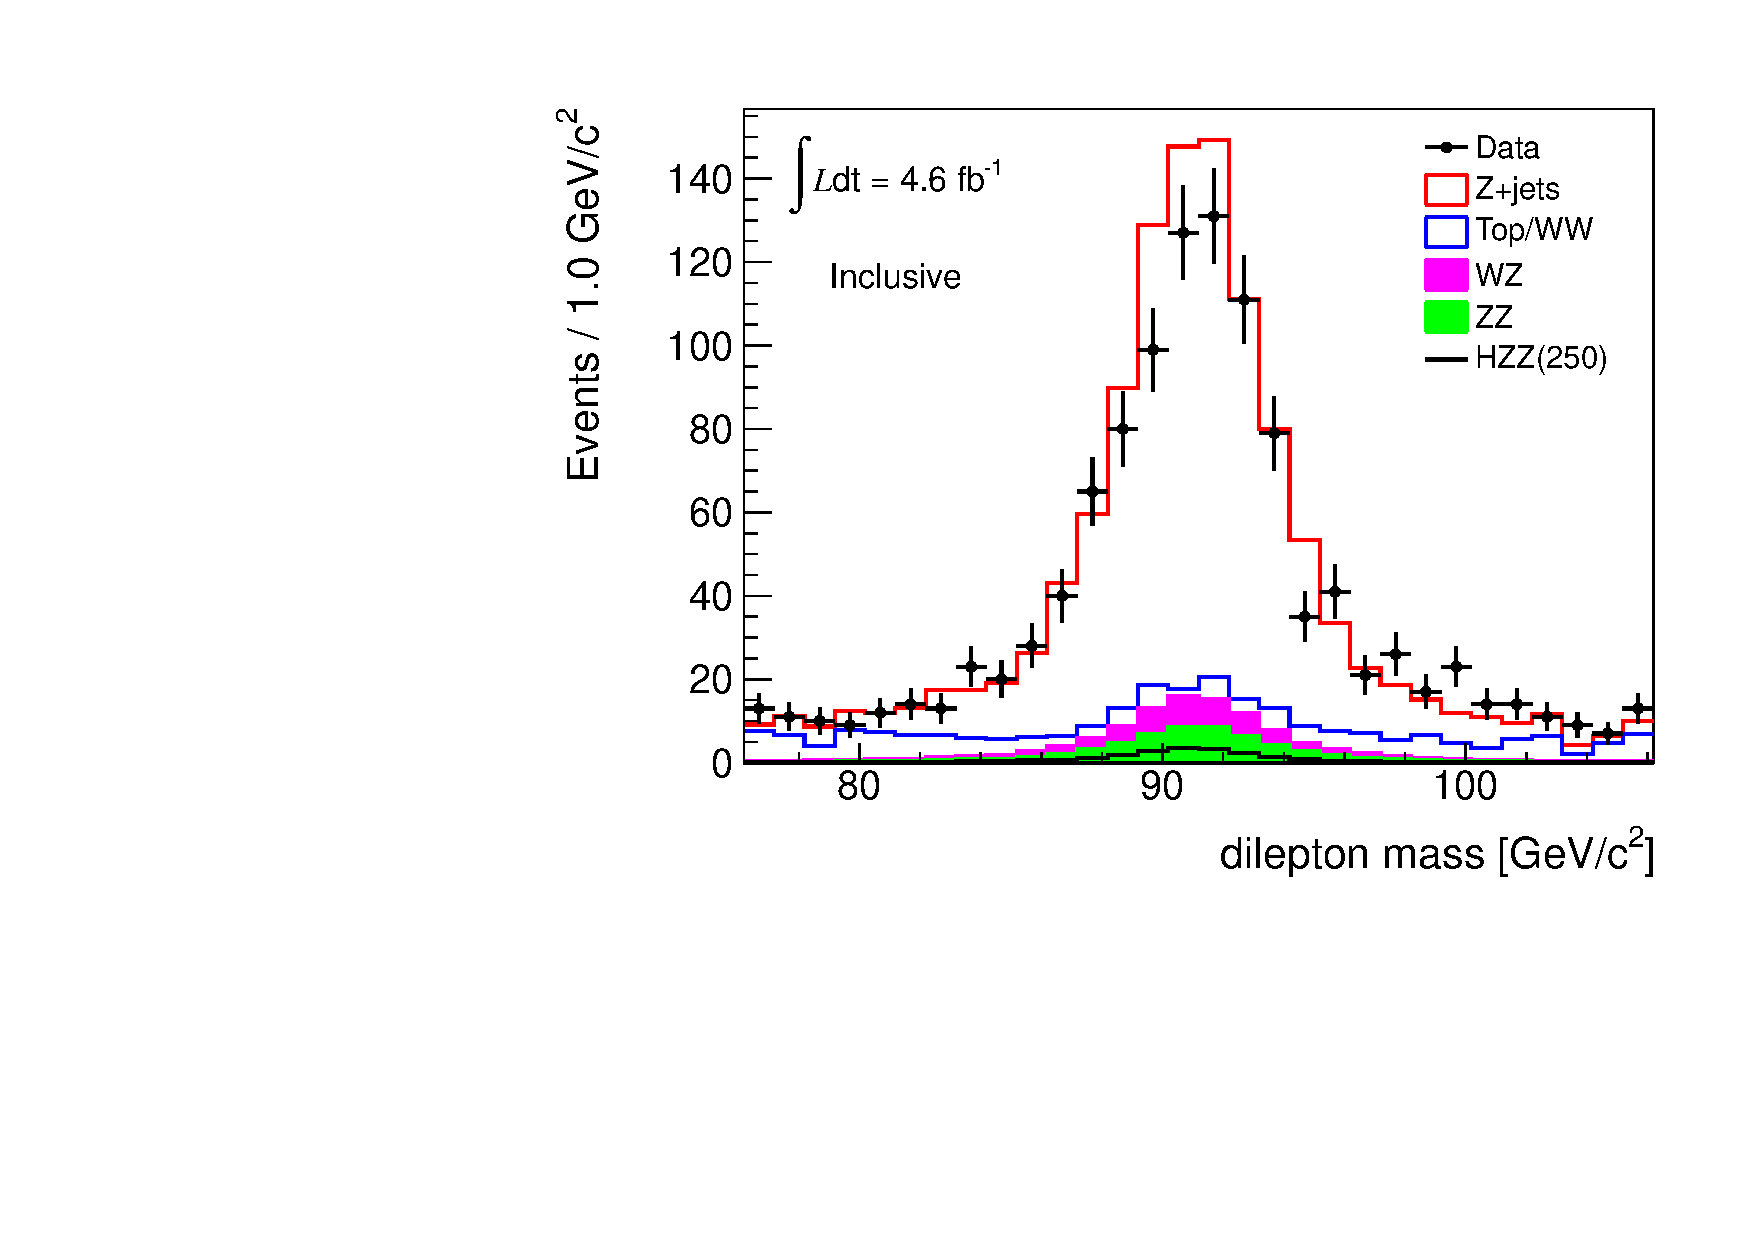
\includegraphics[width=.4\textwidth]{figures/presel_mH250_mm_mass_incl.pdf}}
\subfigure[0-Jet]{\label{subfig:zmass_mm_0j}
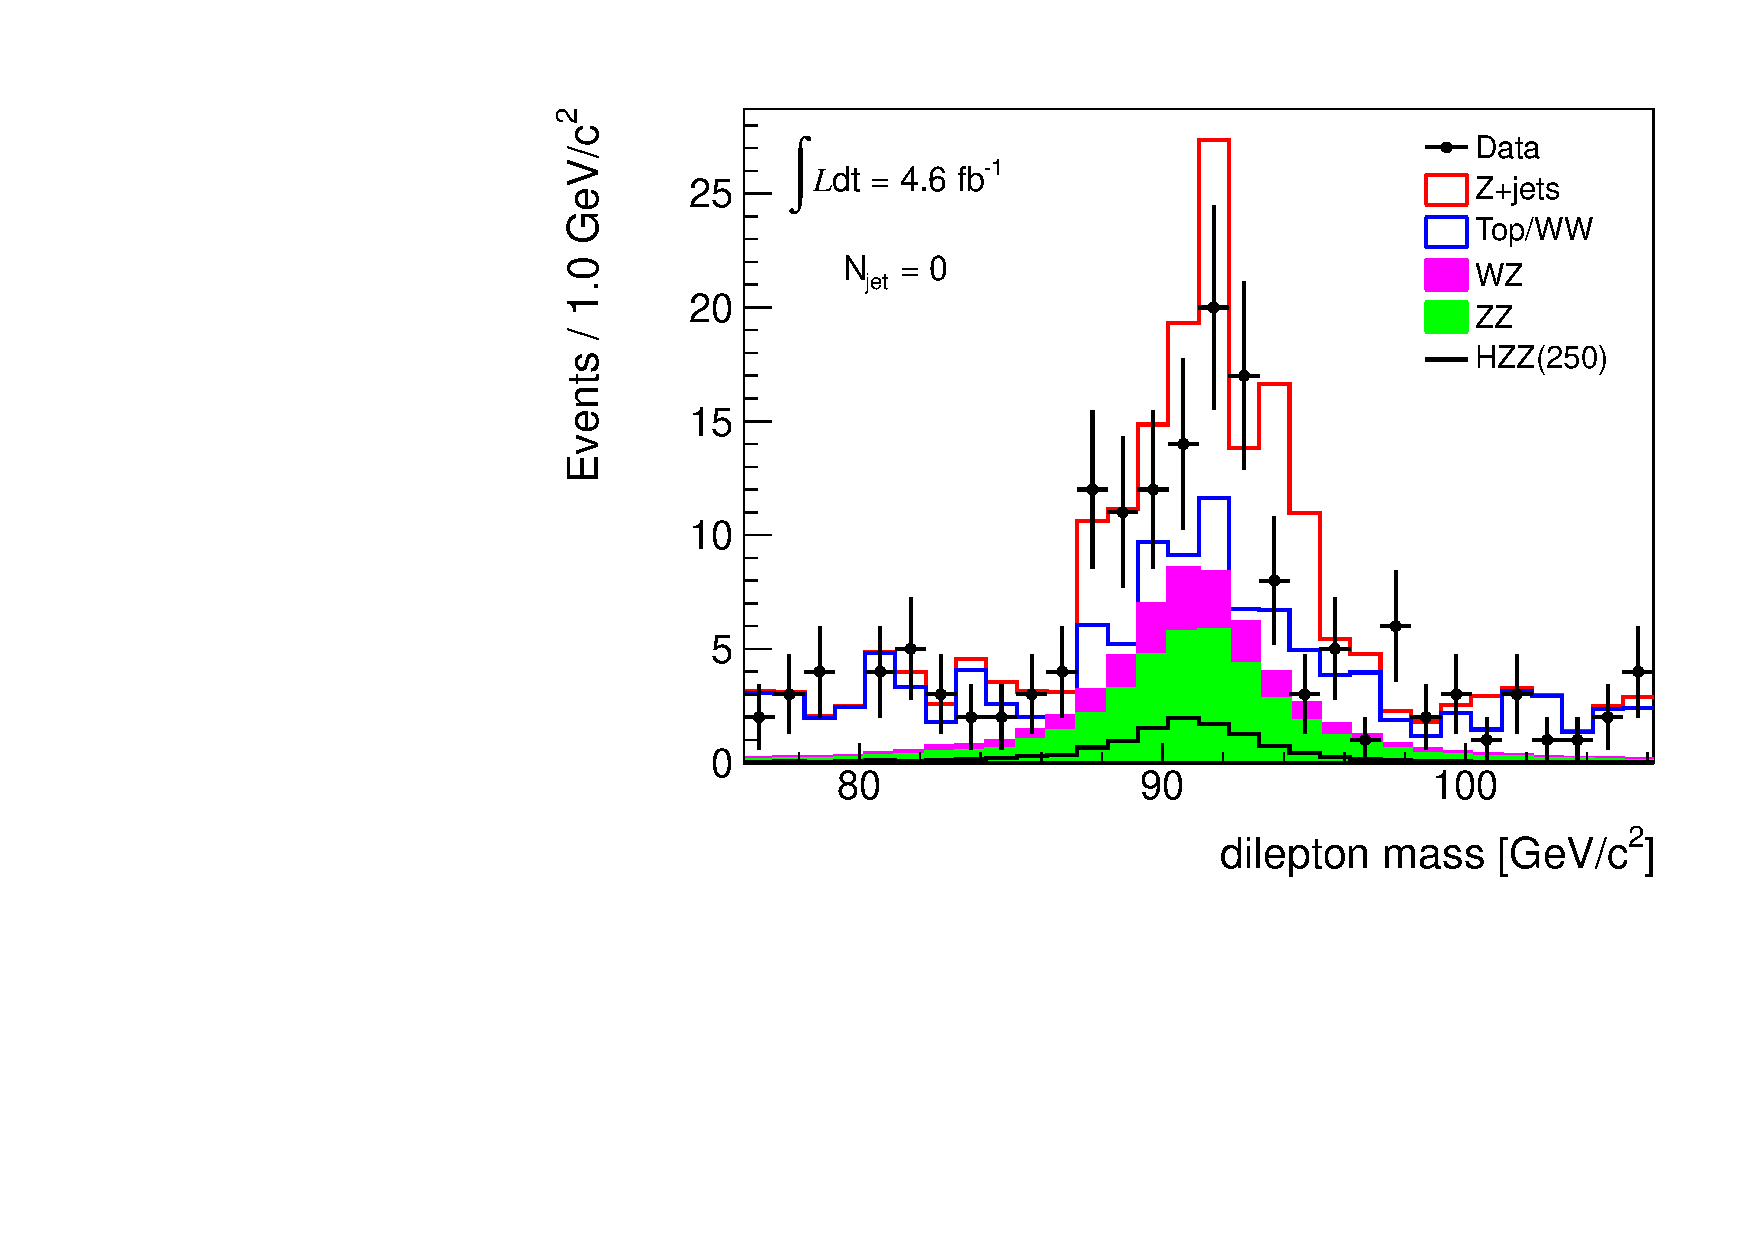
\includegraphics[width=.4\textwidth]{figures/presel_mH250_mm_mass_0j.pdf}} \\
\subfigure[1-Jet]{\label{subfig:zmass_mm_1j}
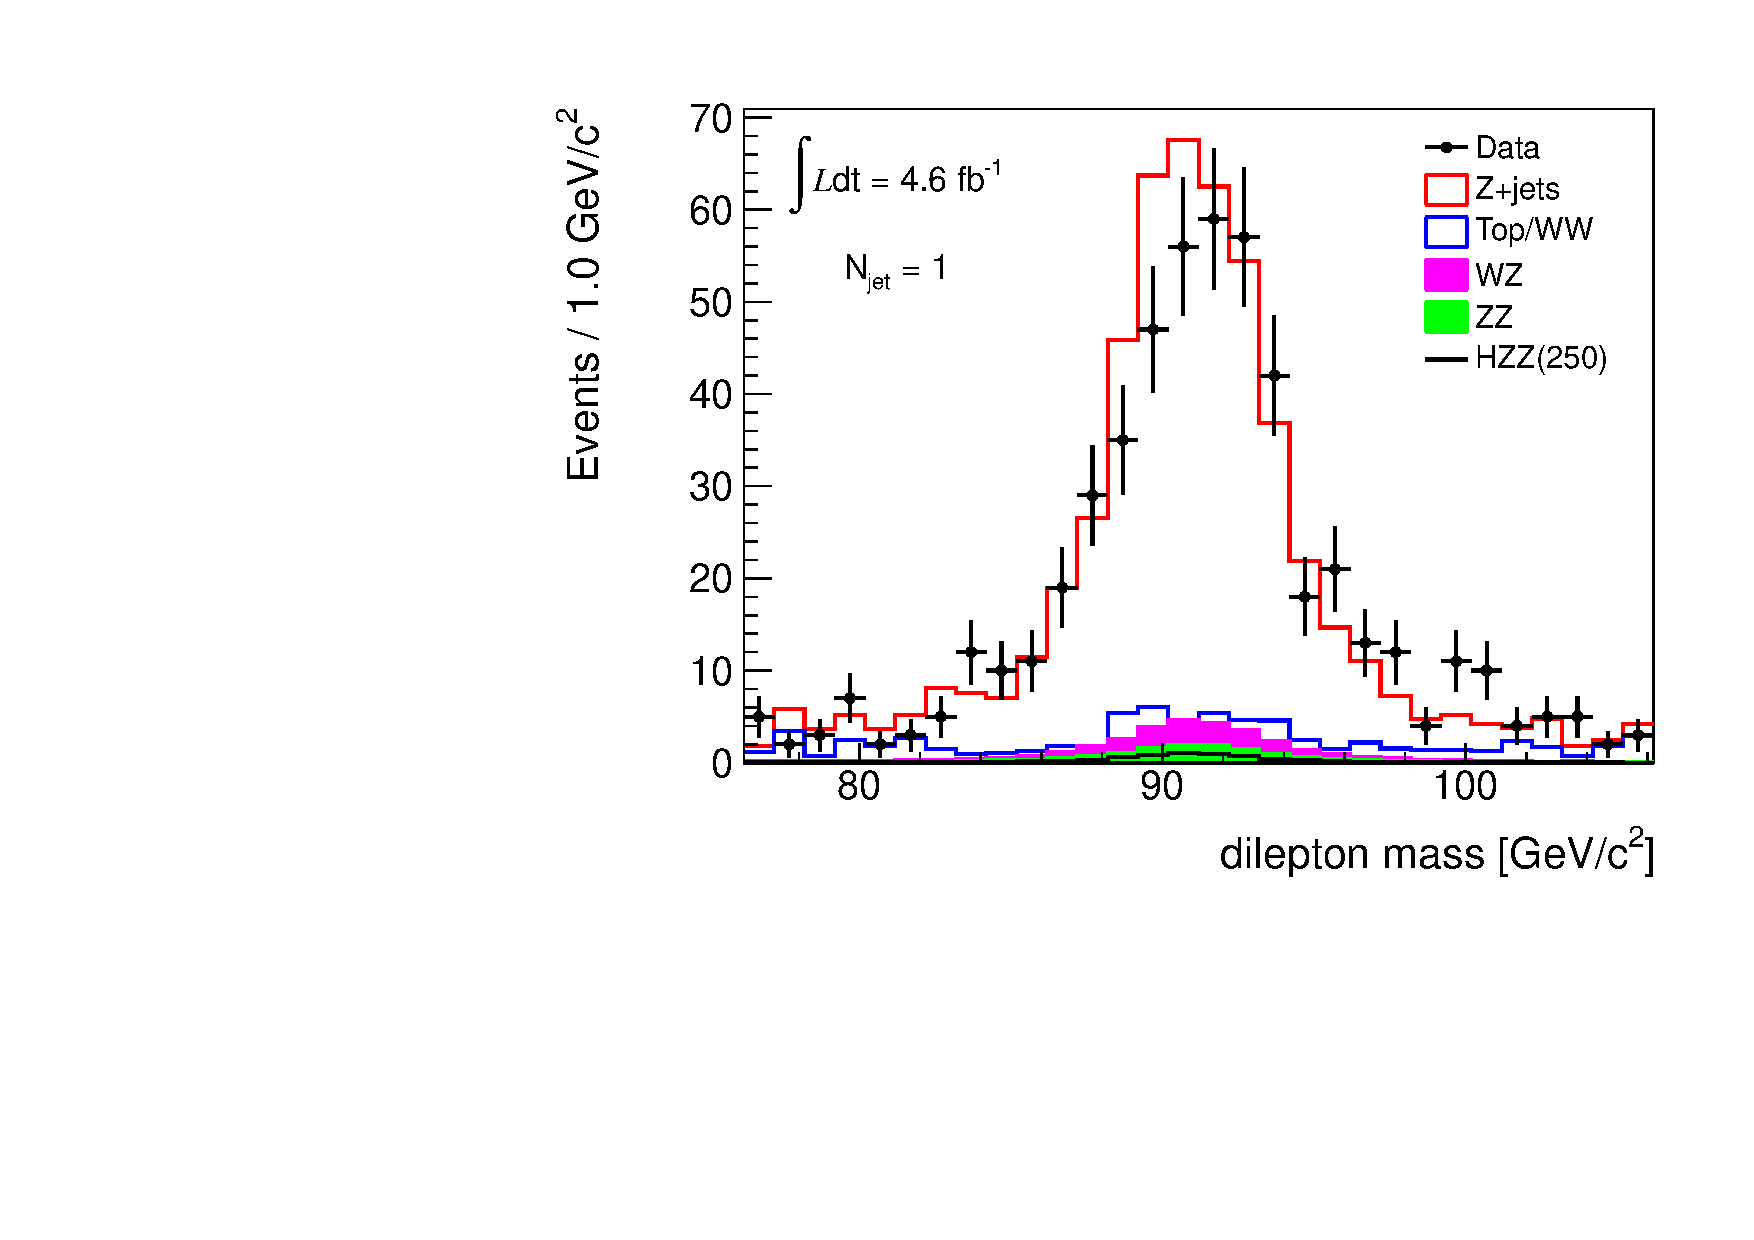
\includegraphics[width=.4\textwidth]{figures/presel_mH250_mm_mass_1j.pdf}}
\subfigure[$\geq$2 Jets]{\label{subfig:zmass_mm_2j}
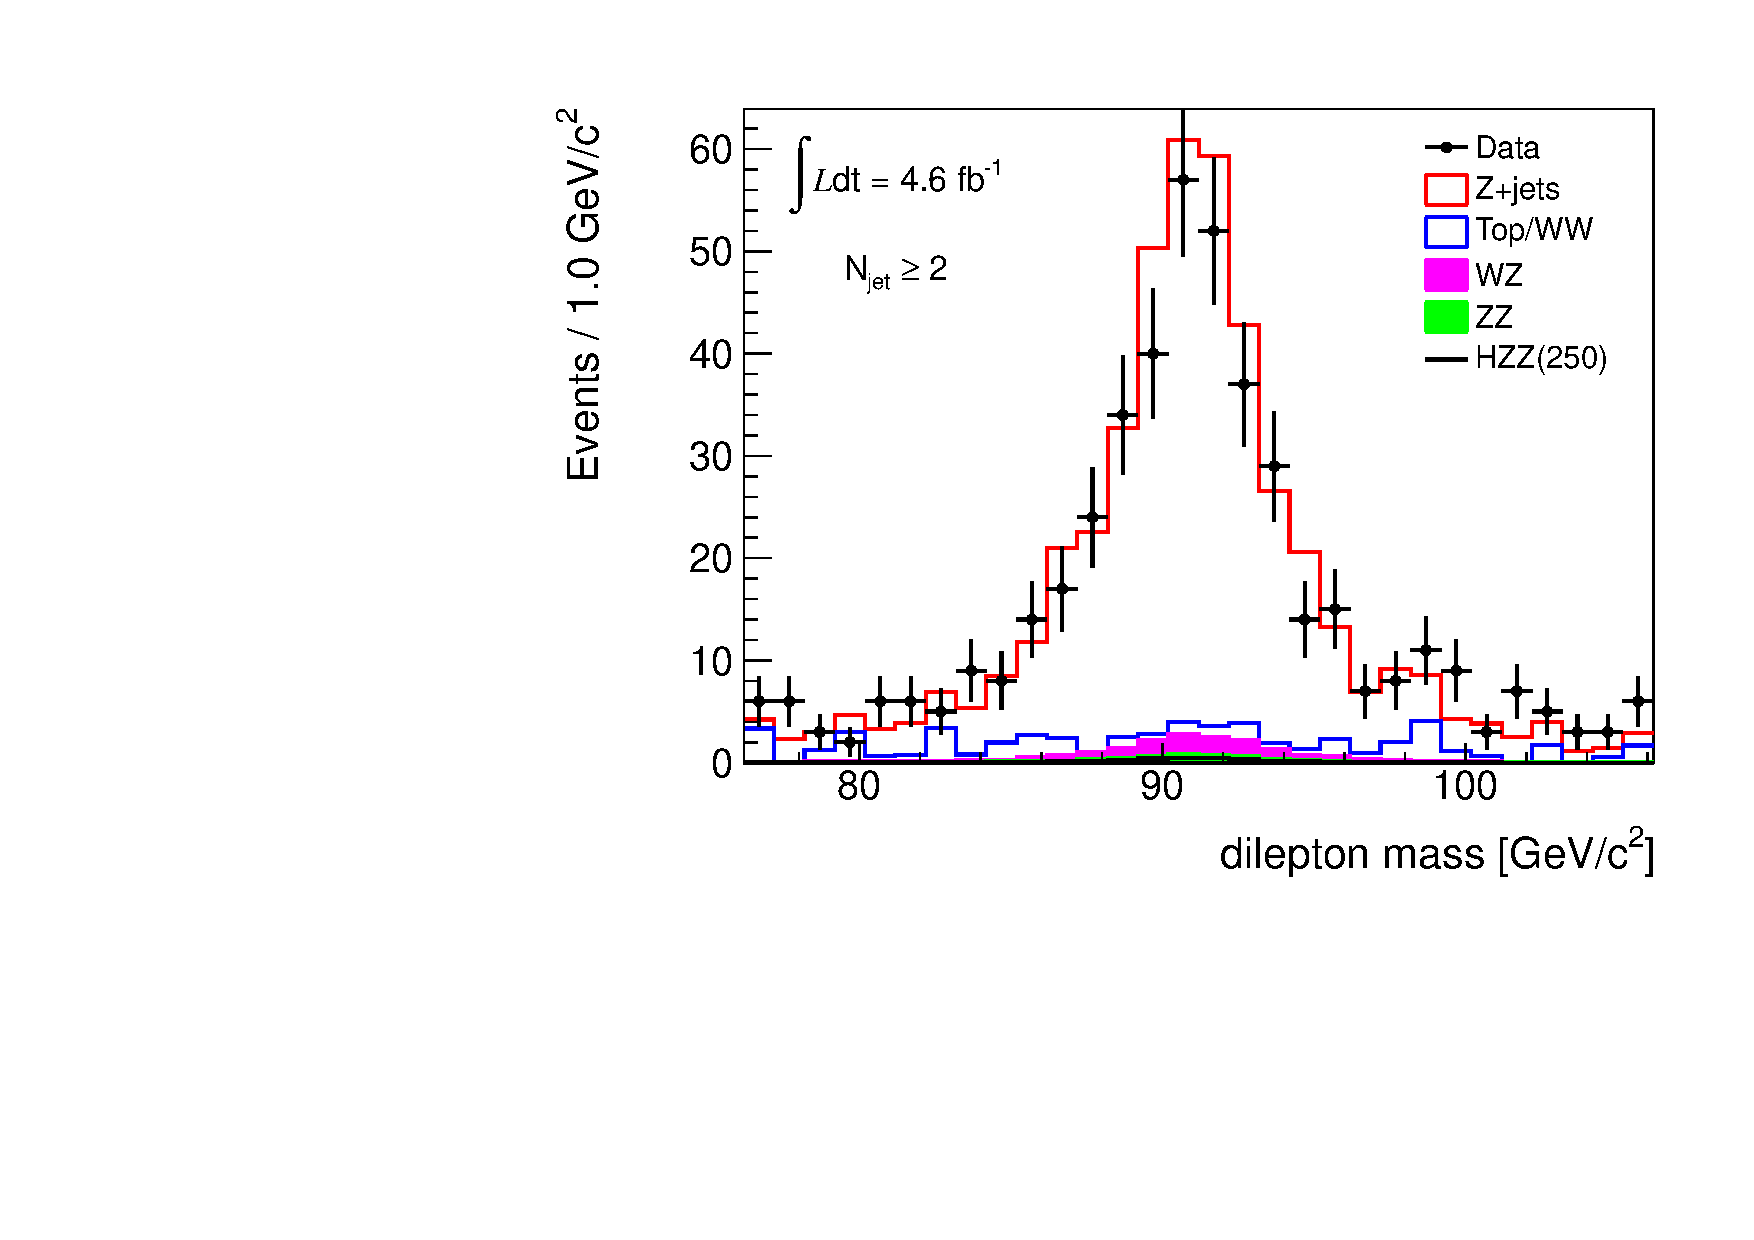
\includegraphics[width=.4\textwidth]{figures/presel_mH250_mm_mass_2j.pdf}}
\caption{Dilepton mass distribution in the muon channel after the $\ZZ$ preselection observed in data corresponding to $2.1$~\ifb data in 
the Inclusive~\subref{subfig:zmass_mm_incl}, 0-Jet~\subref{subfig:zmass_mm_0j}, 1-Jet~\subref{subfig:zmass_mm_1j} and 2-Jet~\subref{subfig:zmass_mm_2j} bins, 
compared to the expected from simulation for signal and background. The MC backgrounds are scaled as appropriate and the photon+jets estimate of the 
Z+jets background is added to the stack.}
\label{fig:zmass_zzpresel_mm}
\end{center}
\end{figure}
%%%%%%%%

%%%%%%%%
\begin{figure}[!hbtp]
\begin{center}
\subfigure[Inclusive]{\label{subfig:zmass_ee_incl}
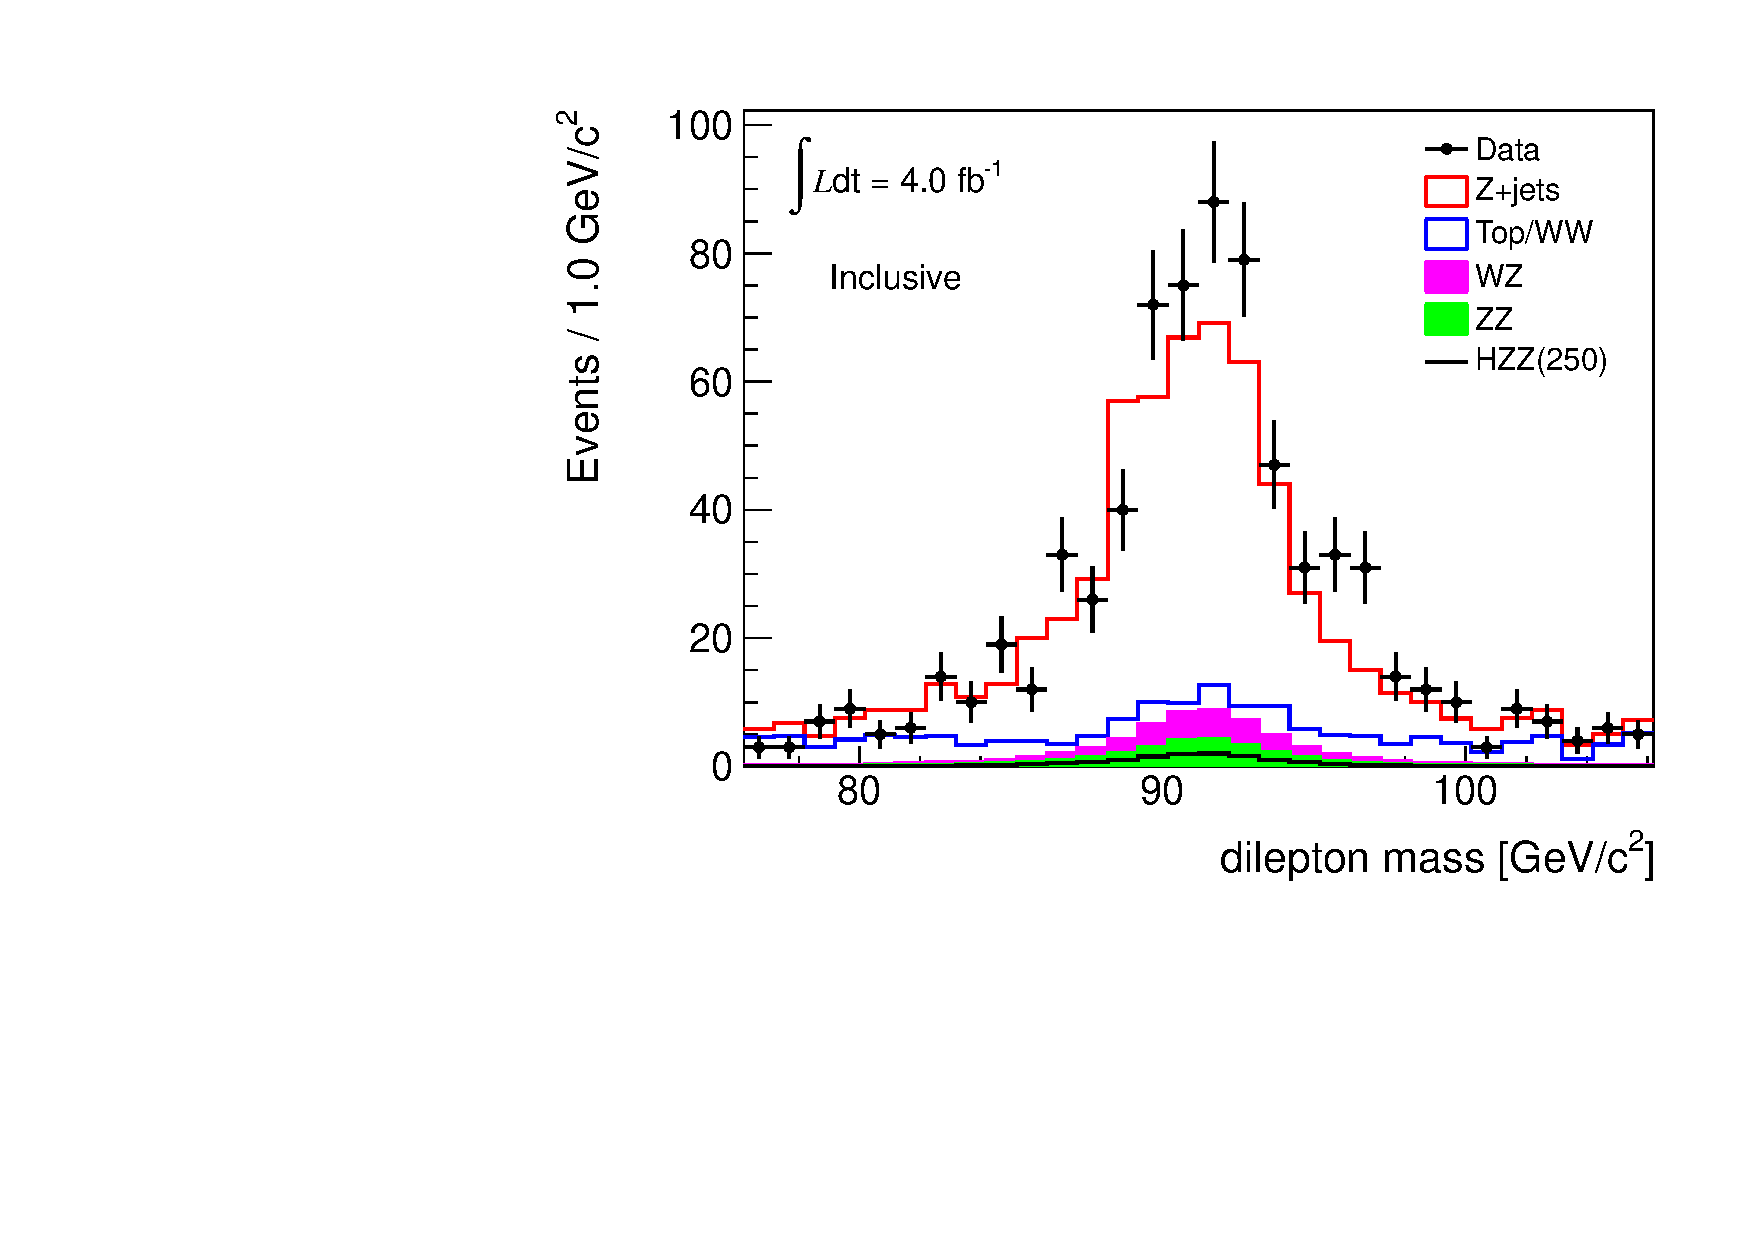
\includegraphics[width=.4\textwidth]{figures/presel_mH250_ee_mass_incl.pdf}}
\subfigure[0-Jet]{\label{subfig:zmass_ee_0j}
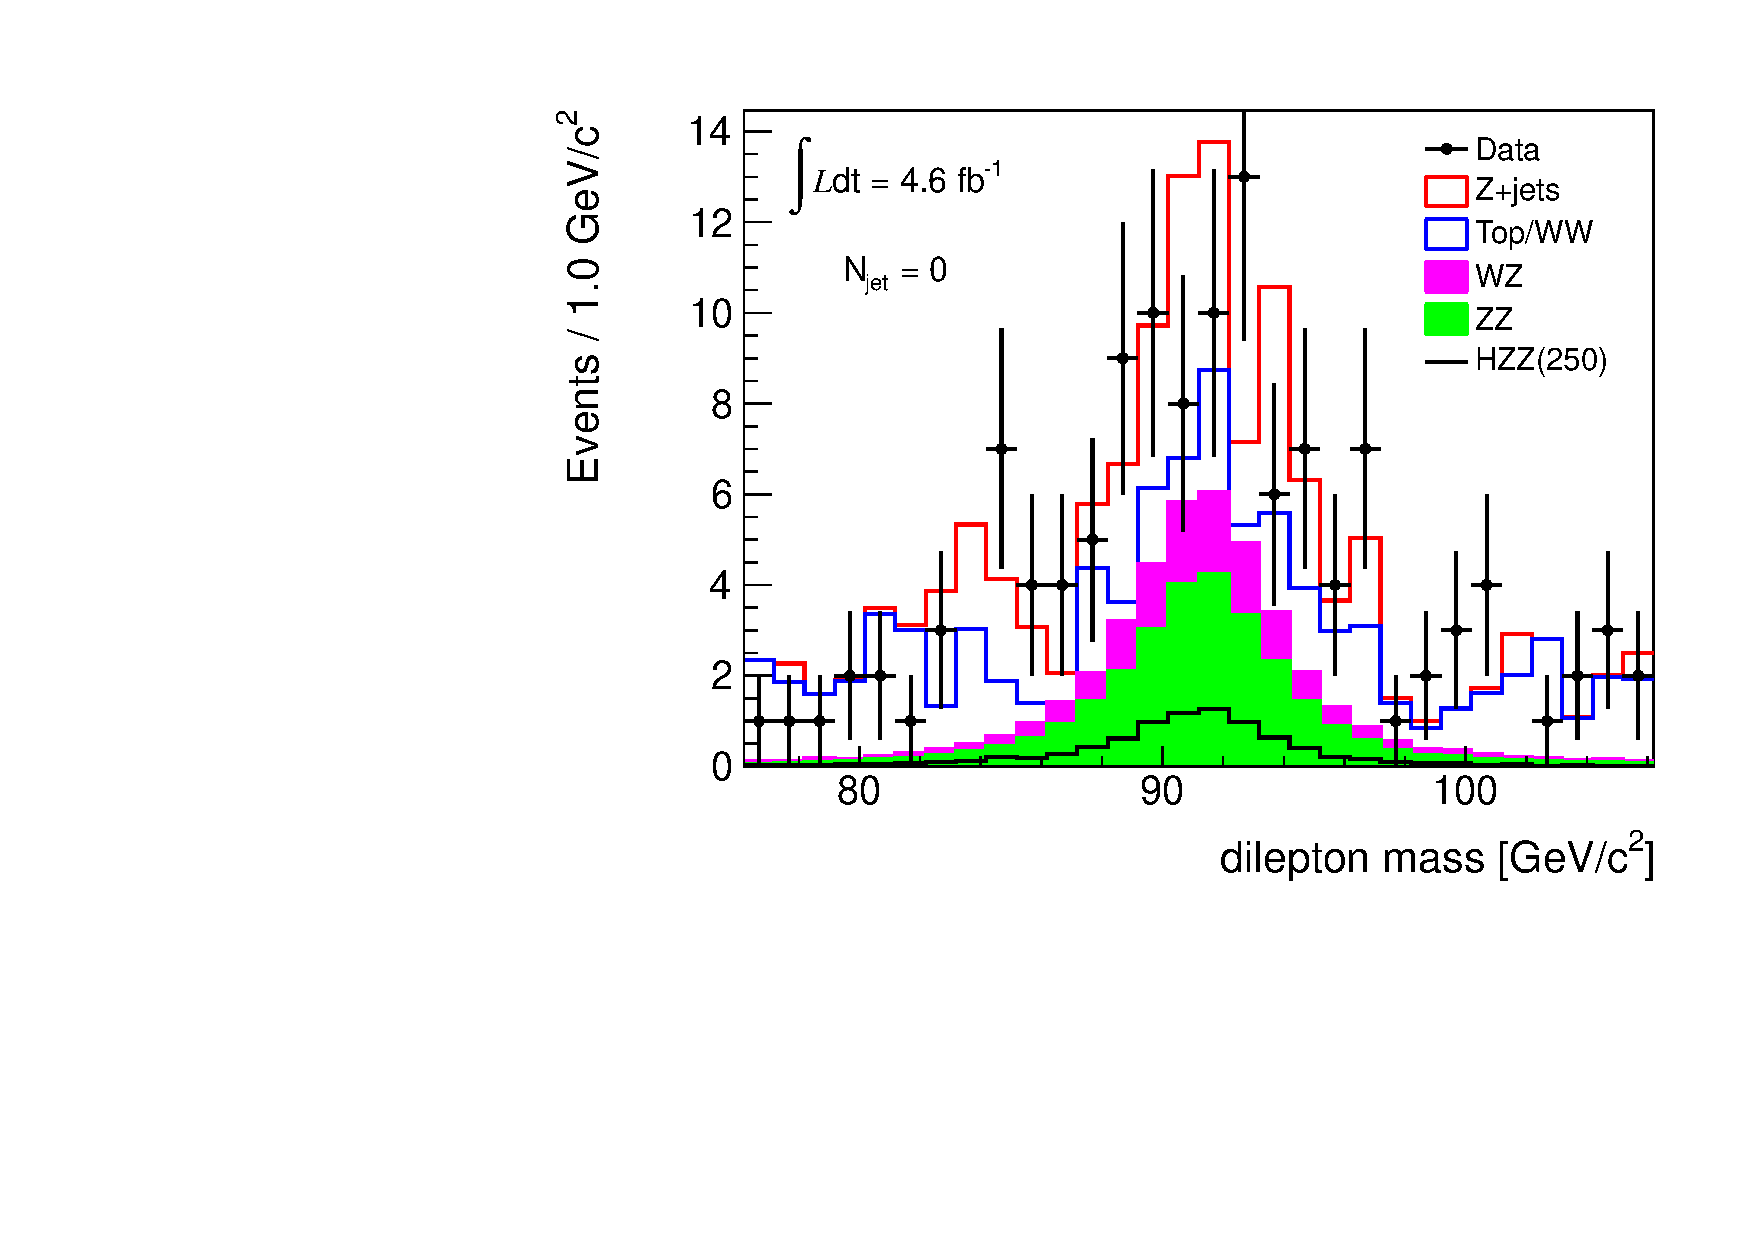
\includegraphics[width=.4\textwidth]{figures/presel_mH250_ee_mass_0j.pdf}} \\
\subfigure[1-Jet]{\label{subfig:zmass_ee_1j}
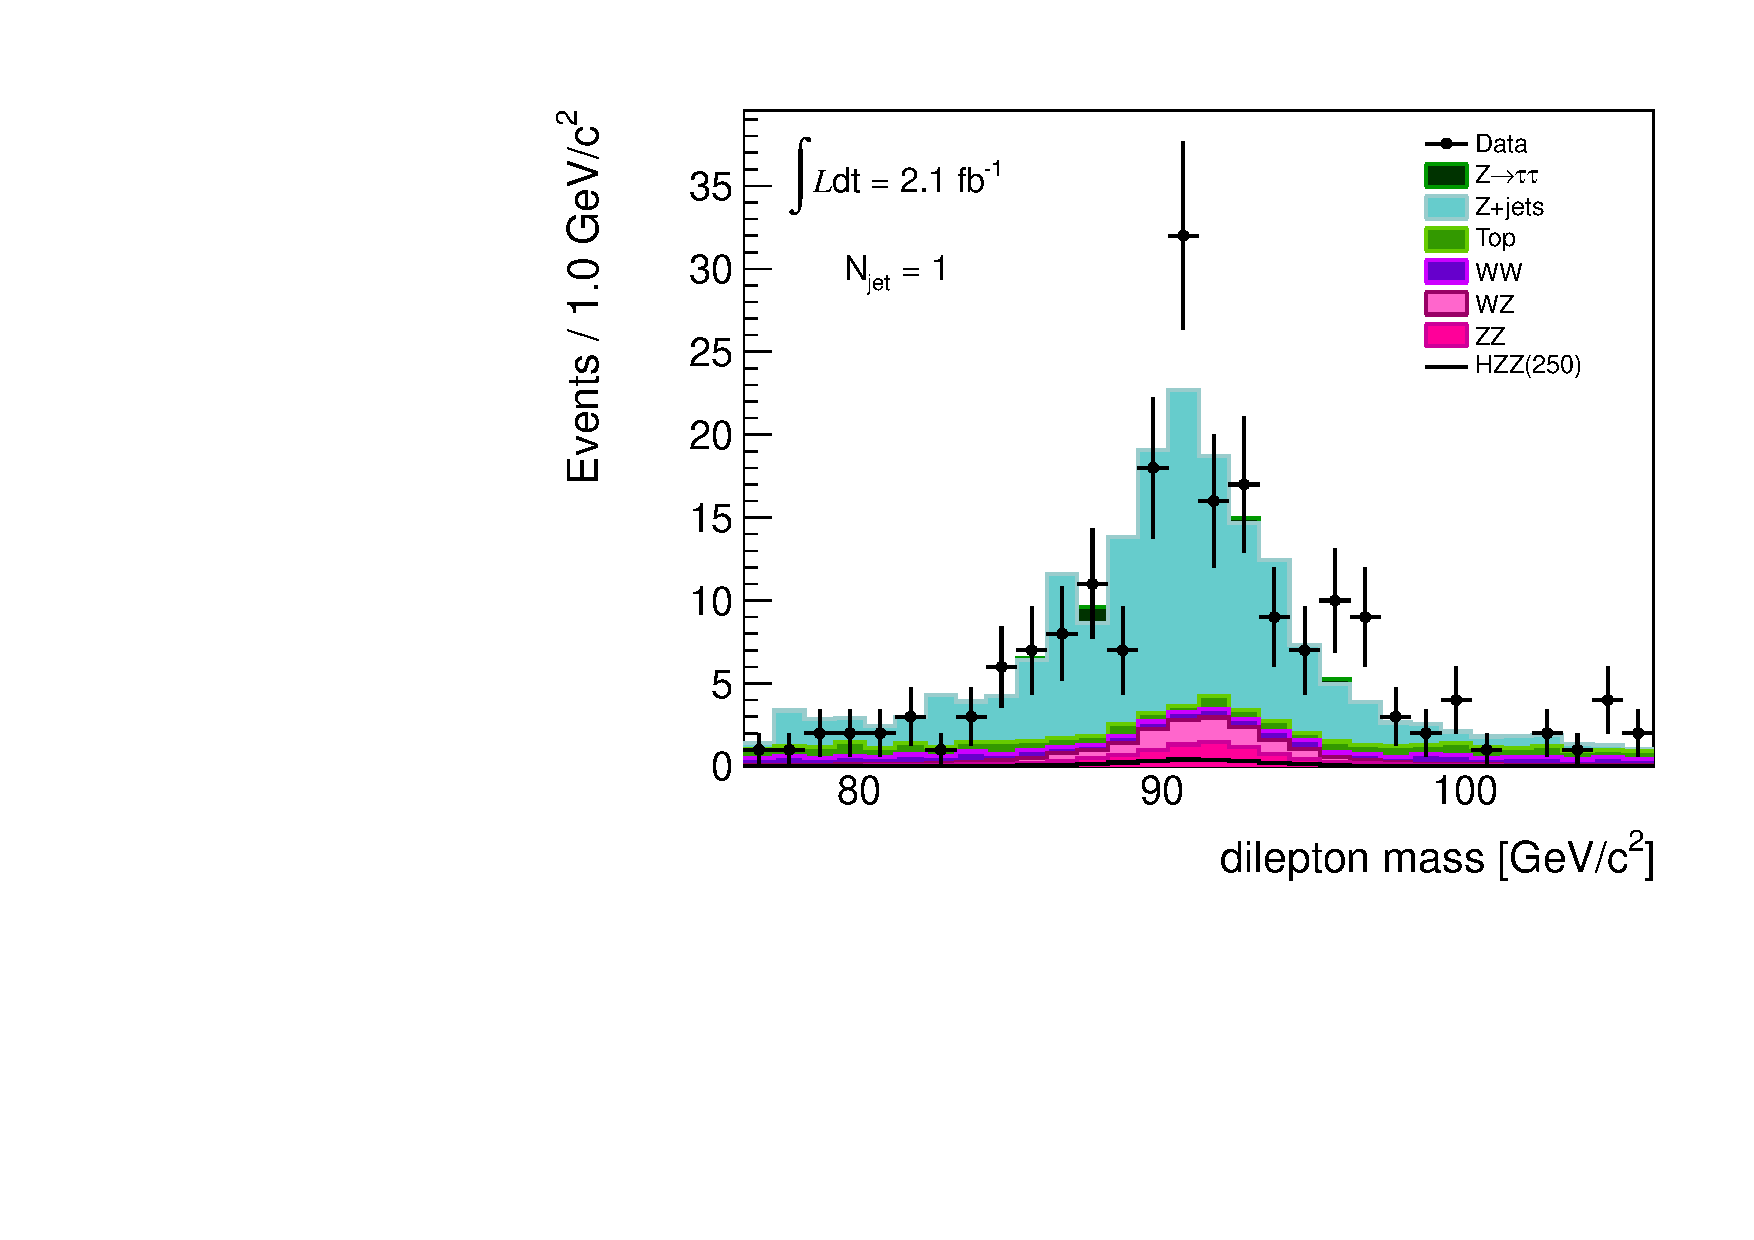
\includegraphics[width=.4\textwidth]{figures/presel_mH250_ee_mass_1j.pdf}}
\subfigure[$\geq$2 Jets]{\label{subfig:zmass_ee_2j}
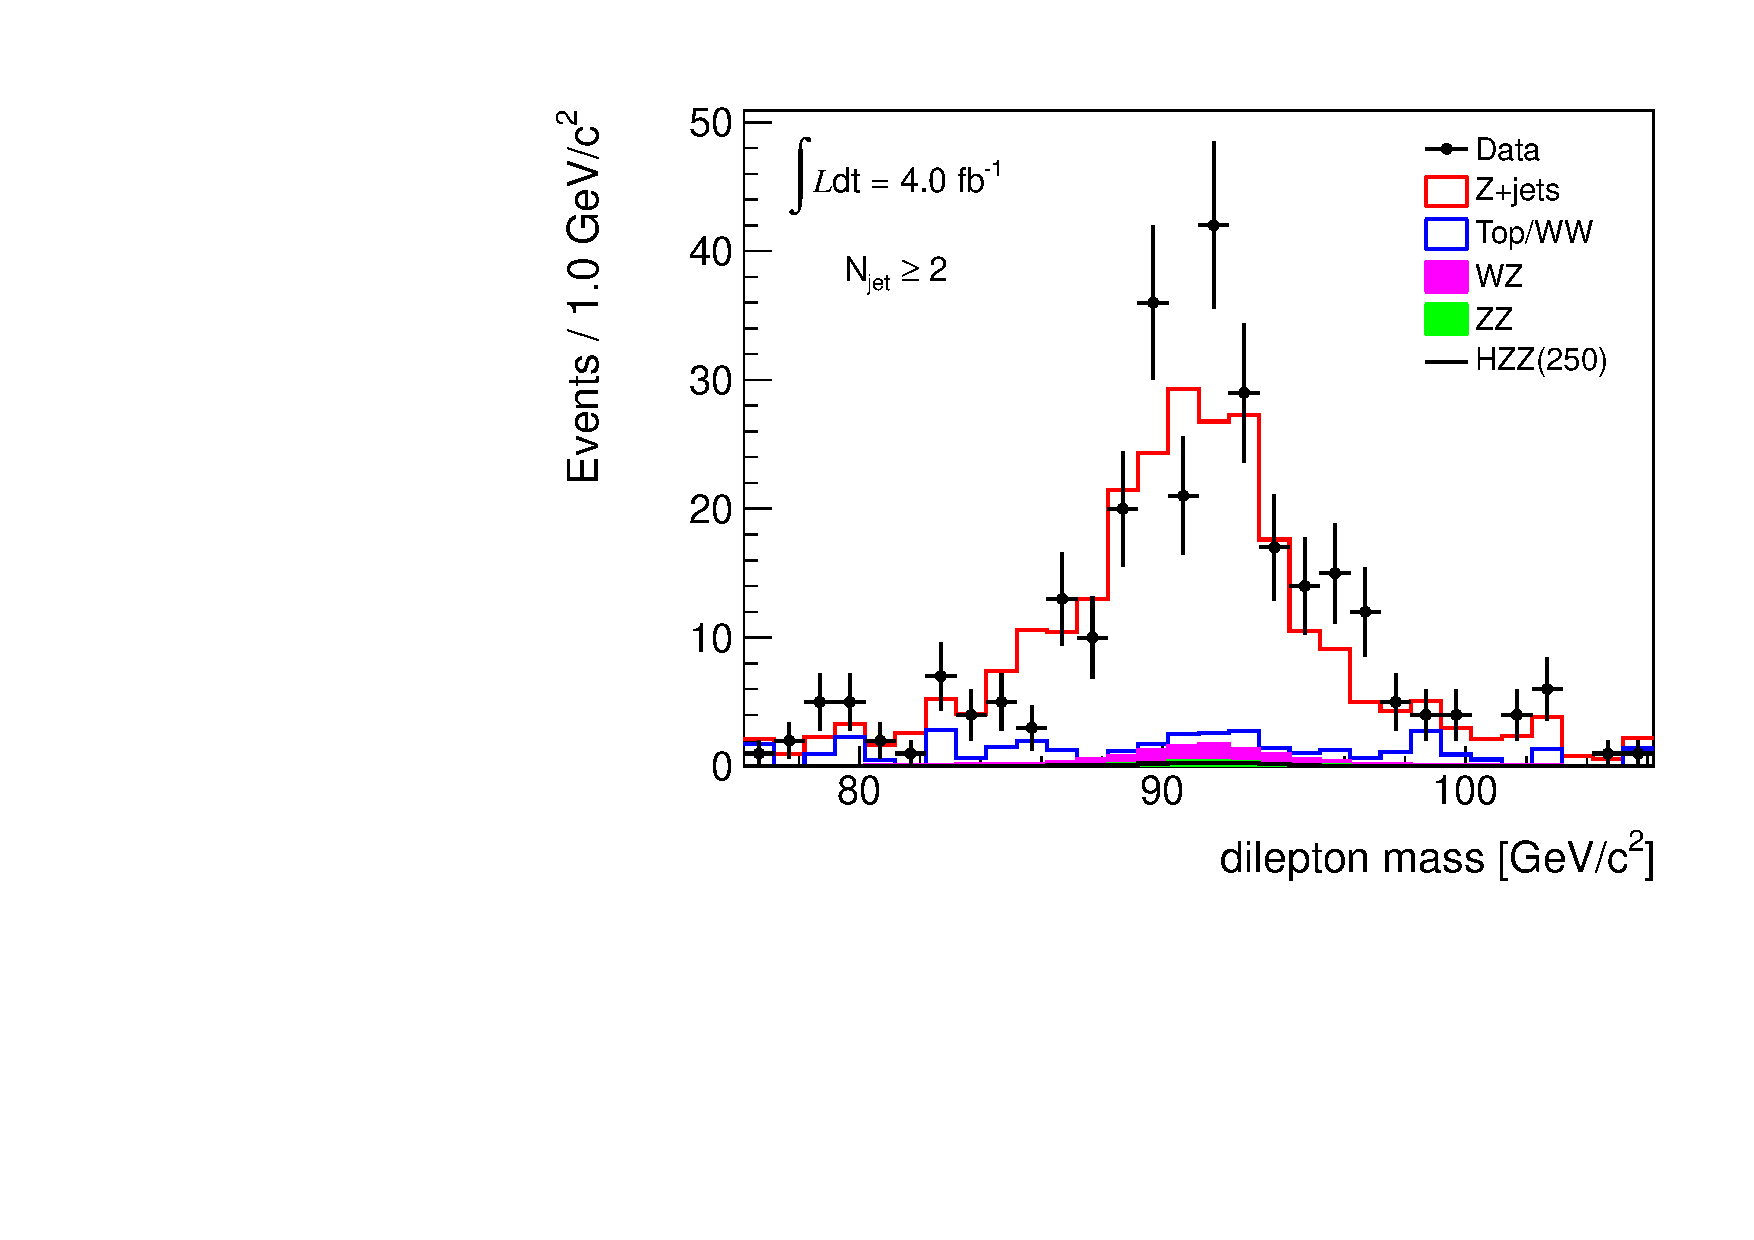
\includegraphics[width=.4\textwidth]{figures/presel_mH250_ee_mass_2j.pdf}}
\caption{Dilepton mass distribution in the electron channel after the $\ZZ$ preselection observed in data corresponding to $2.1$~\ifb data in 
the Inclusive~\subref{subfig:zmass_ee_incl}, 0-Jet~\subref{subfig:zmass_ee_0j}, 1-Jet~\subref{subfig:zmass_ee_1j} and 2-Jet~\subref{subfig:zmass_ee_2j} bins, 
compared to the expected from simulation for signal and background. The MC backgrounds are scaled as appropriate and the photon+jets estimate of the 
Z+jets background is added to the stack.}
\label{fig:zmass_zzpresel_ee}
\end{center}
\end{figure}
%%%%%%%%

%%%%%%%%
\begin{figure}[!hbtp]
\begin{center}
\subfigure[Inclusive]{\label{subfig:zpt_mm_incl}
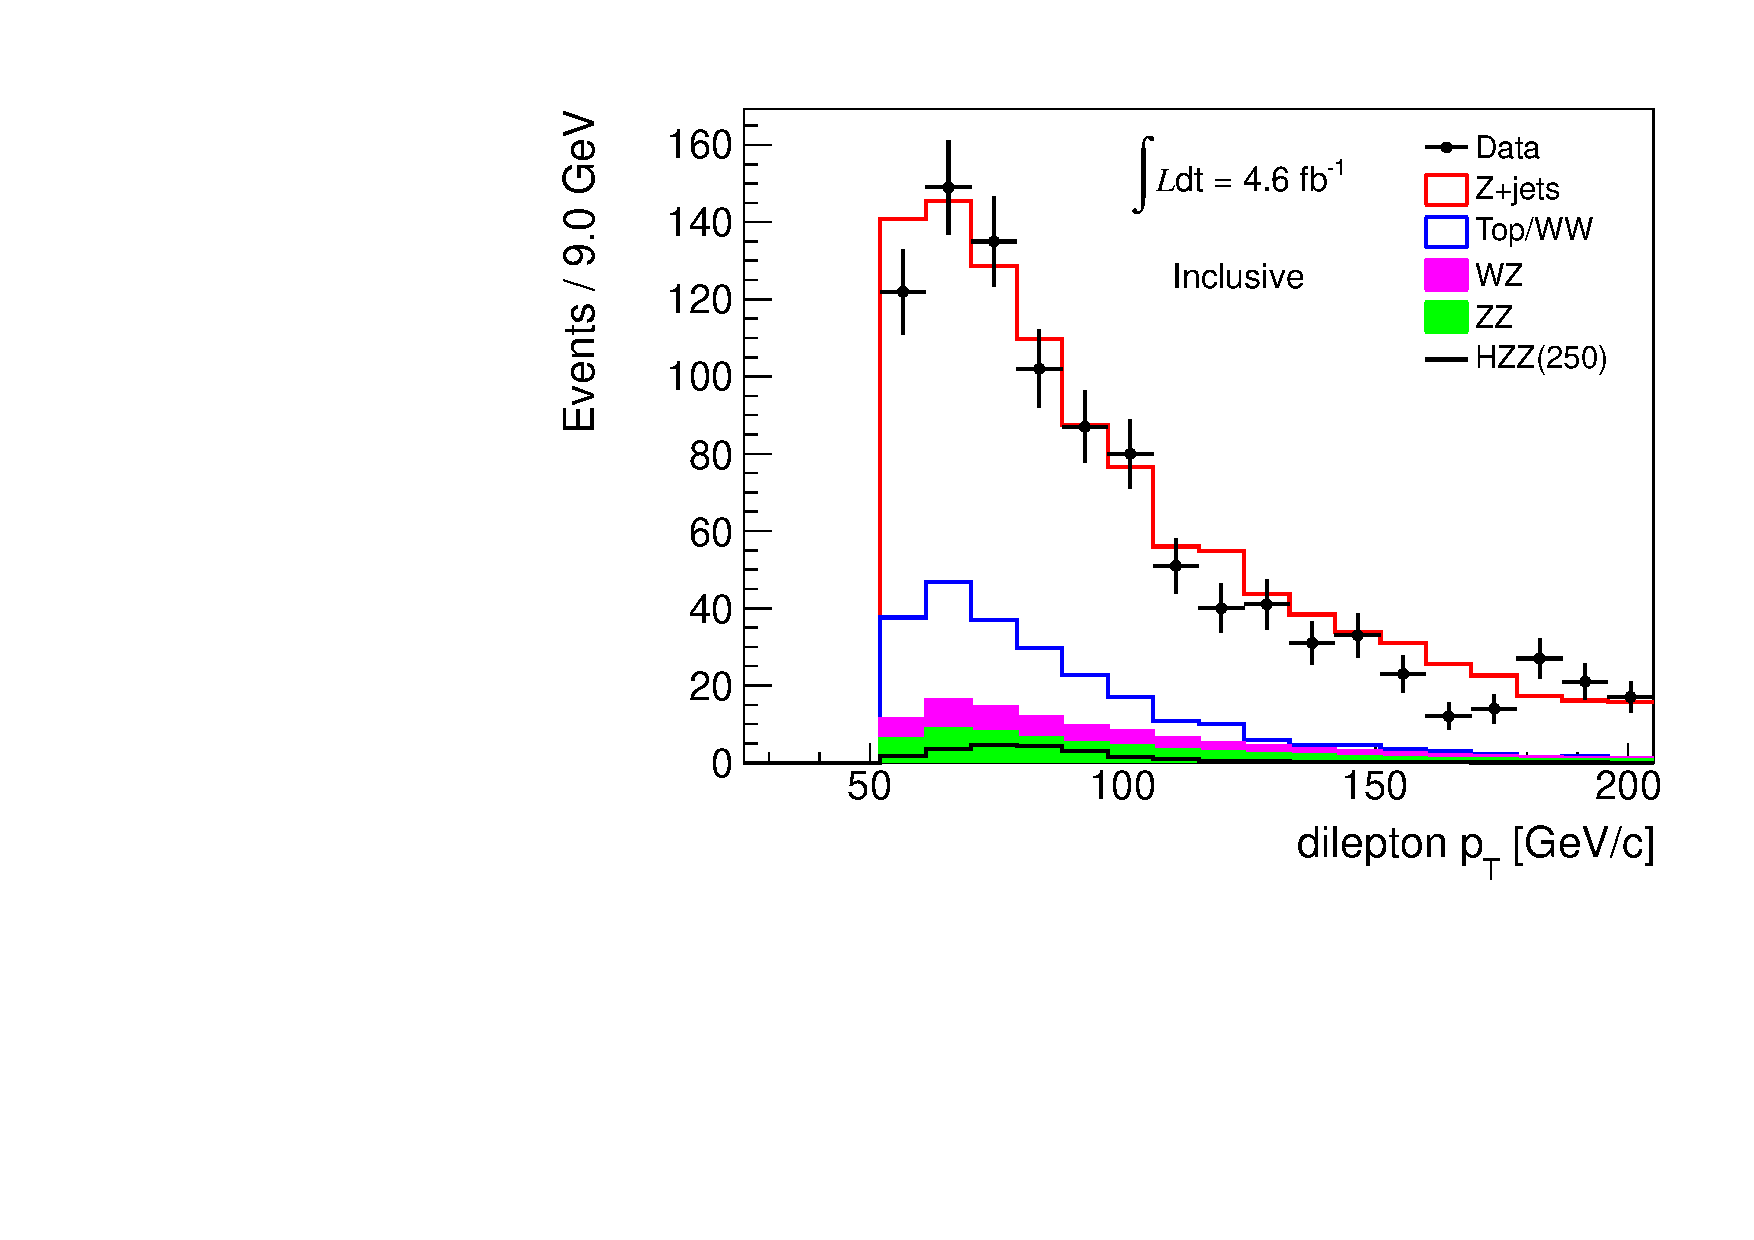
\includegraphics[width=.4\textwidth]{figures/presel_mH250_mm_dileppt_incl.pdf}}
\subfigure[0-Jet]{\label{subfig:zpt_mm_0j}
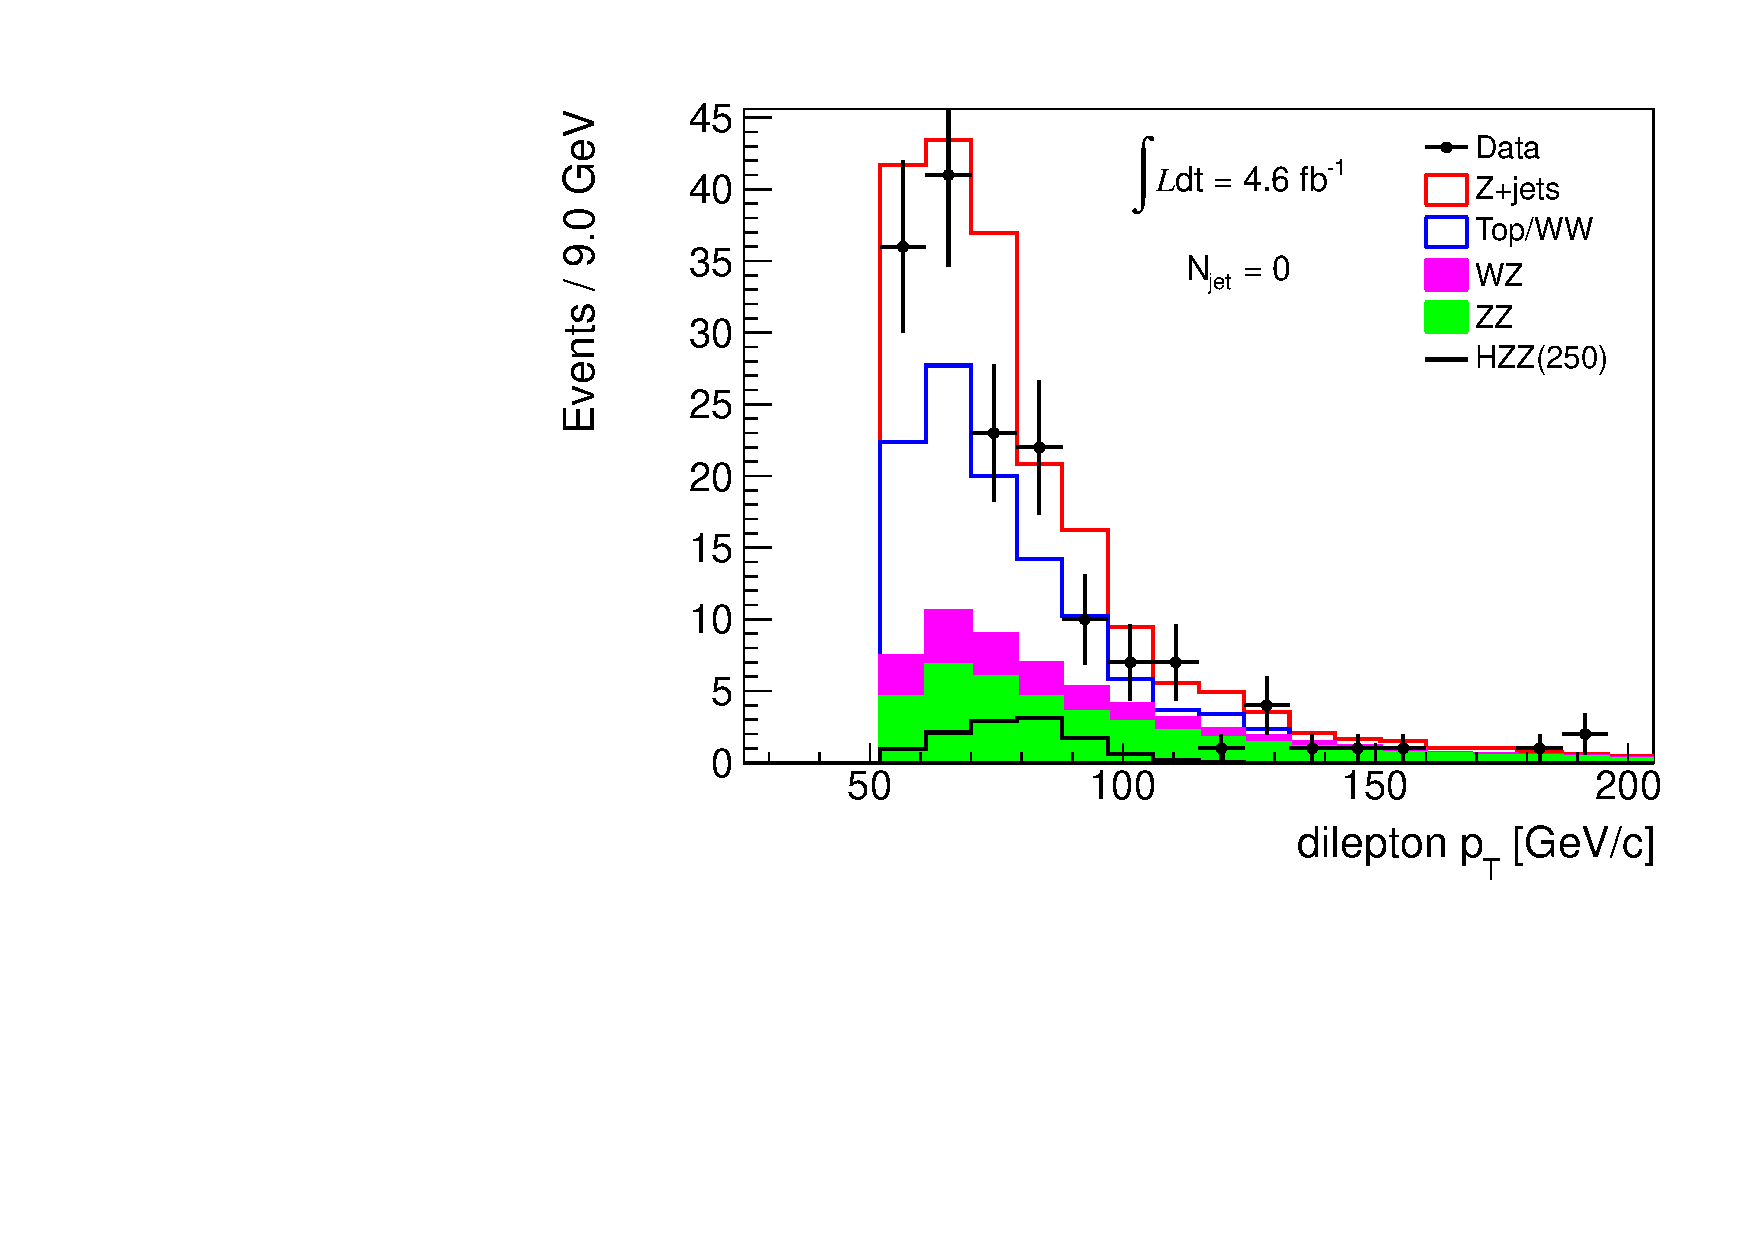
\includegraphics[width=.4\textwidth]{figures/presel_mH250_mm_dileppt_0j.pdf}} \\
\subfigure[1-Jet]{\label{subfig:zpt_mm_1j}
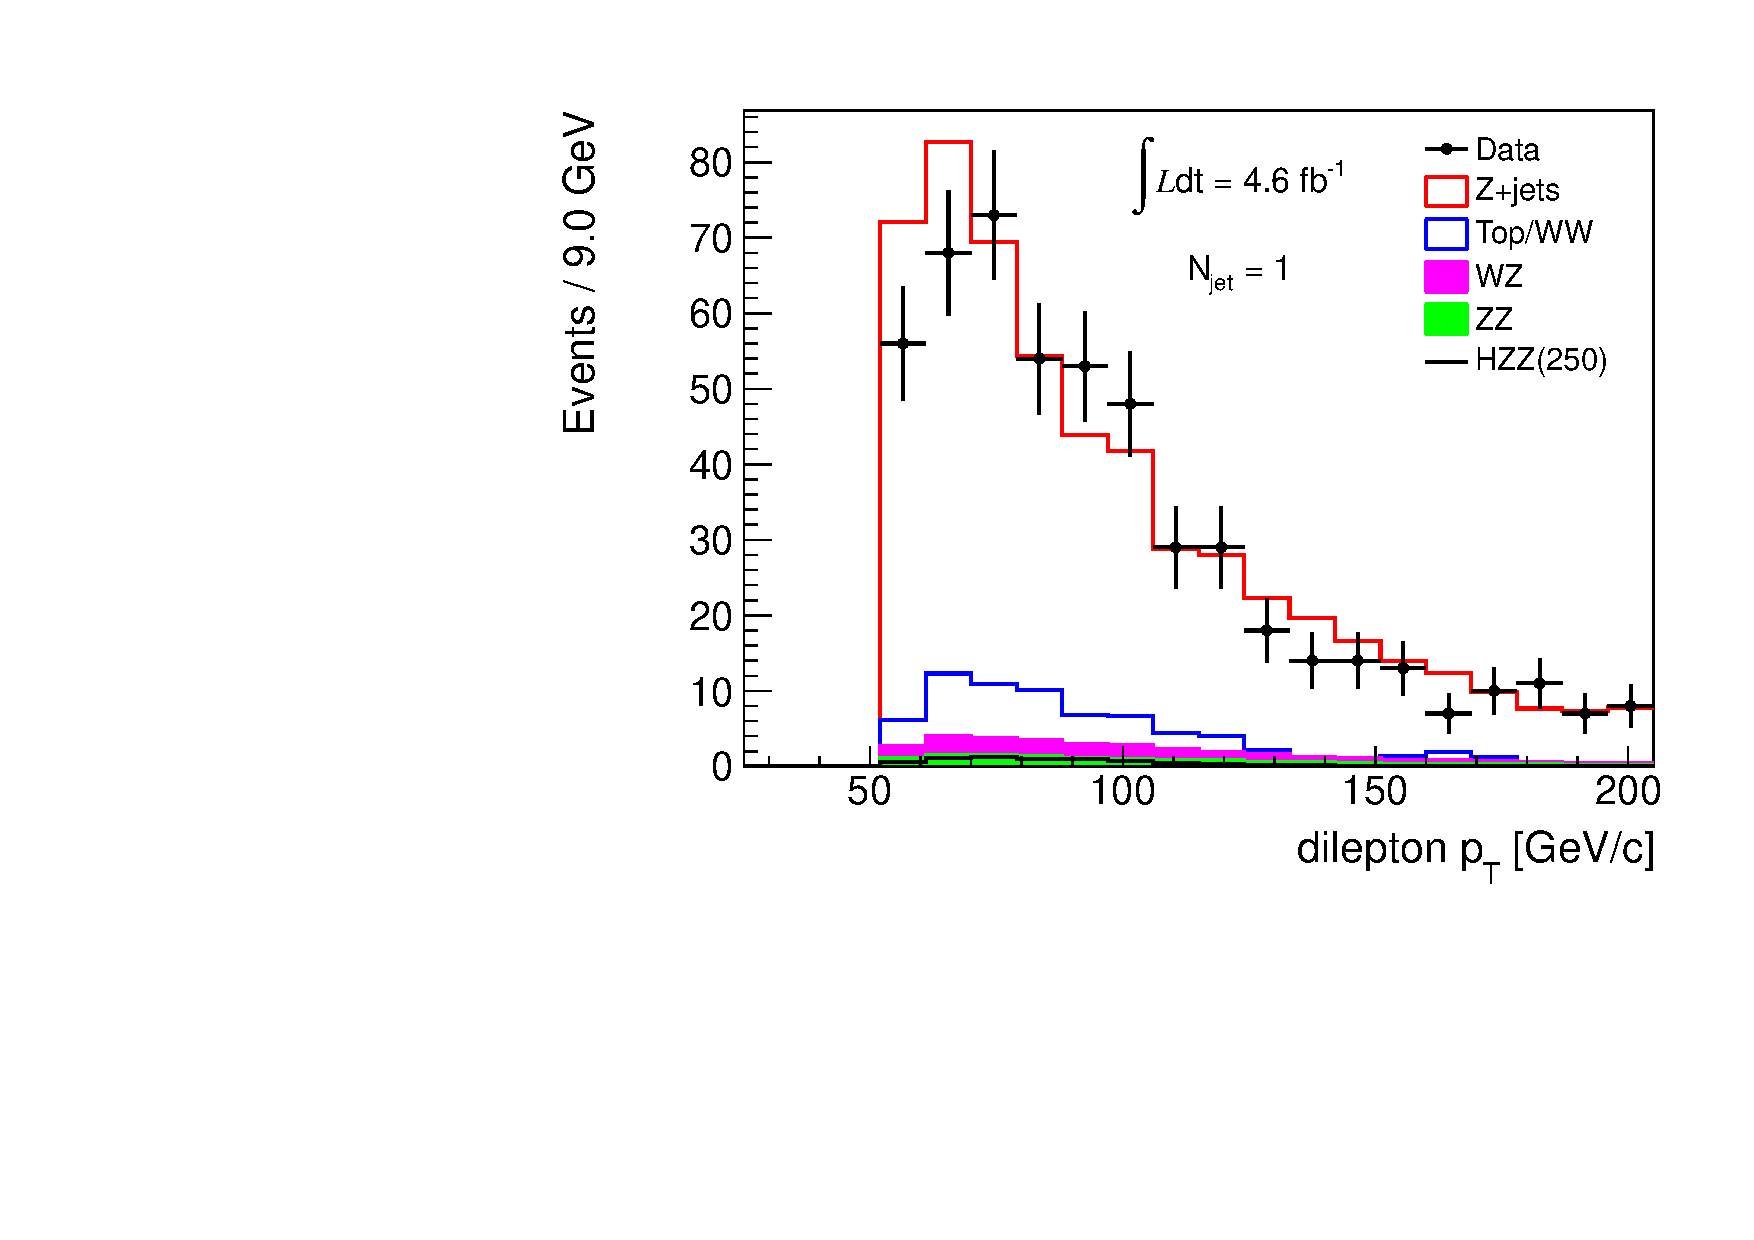
\includegraphics[width=.4\textwidth]{figures/presel_mH250_mm_dileppt_1j.pdf}}
\subfigure[$\geq$2 Jets]{\label{subfig:zpt_mm_2j}
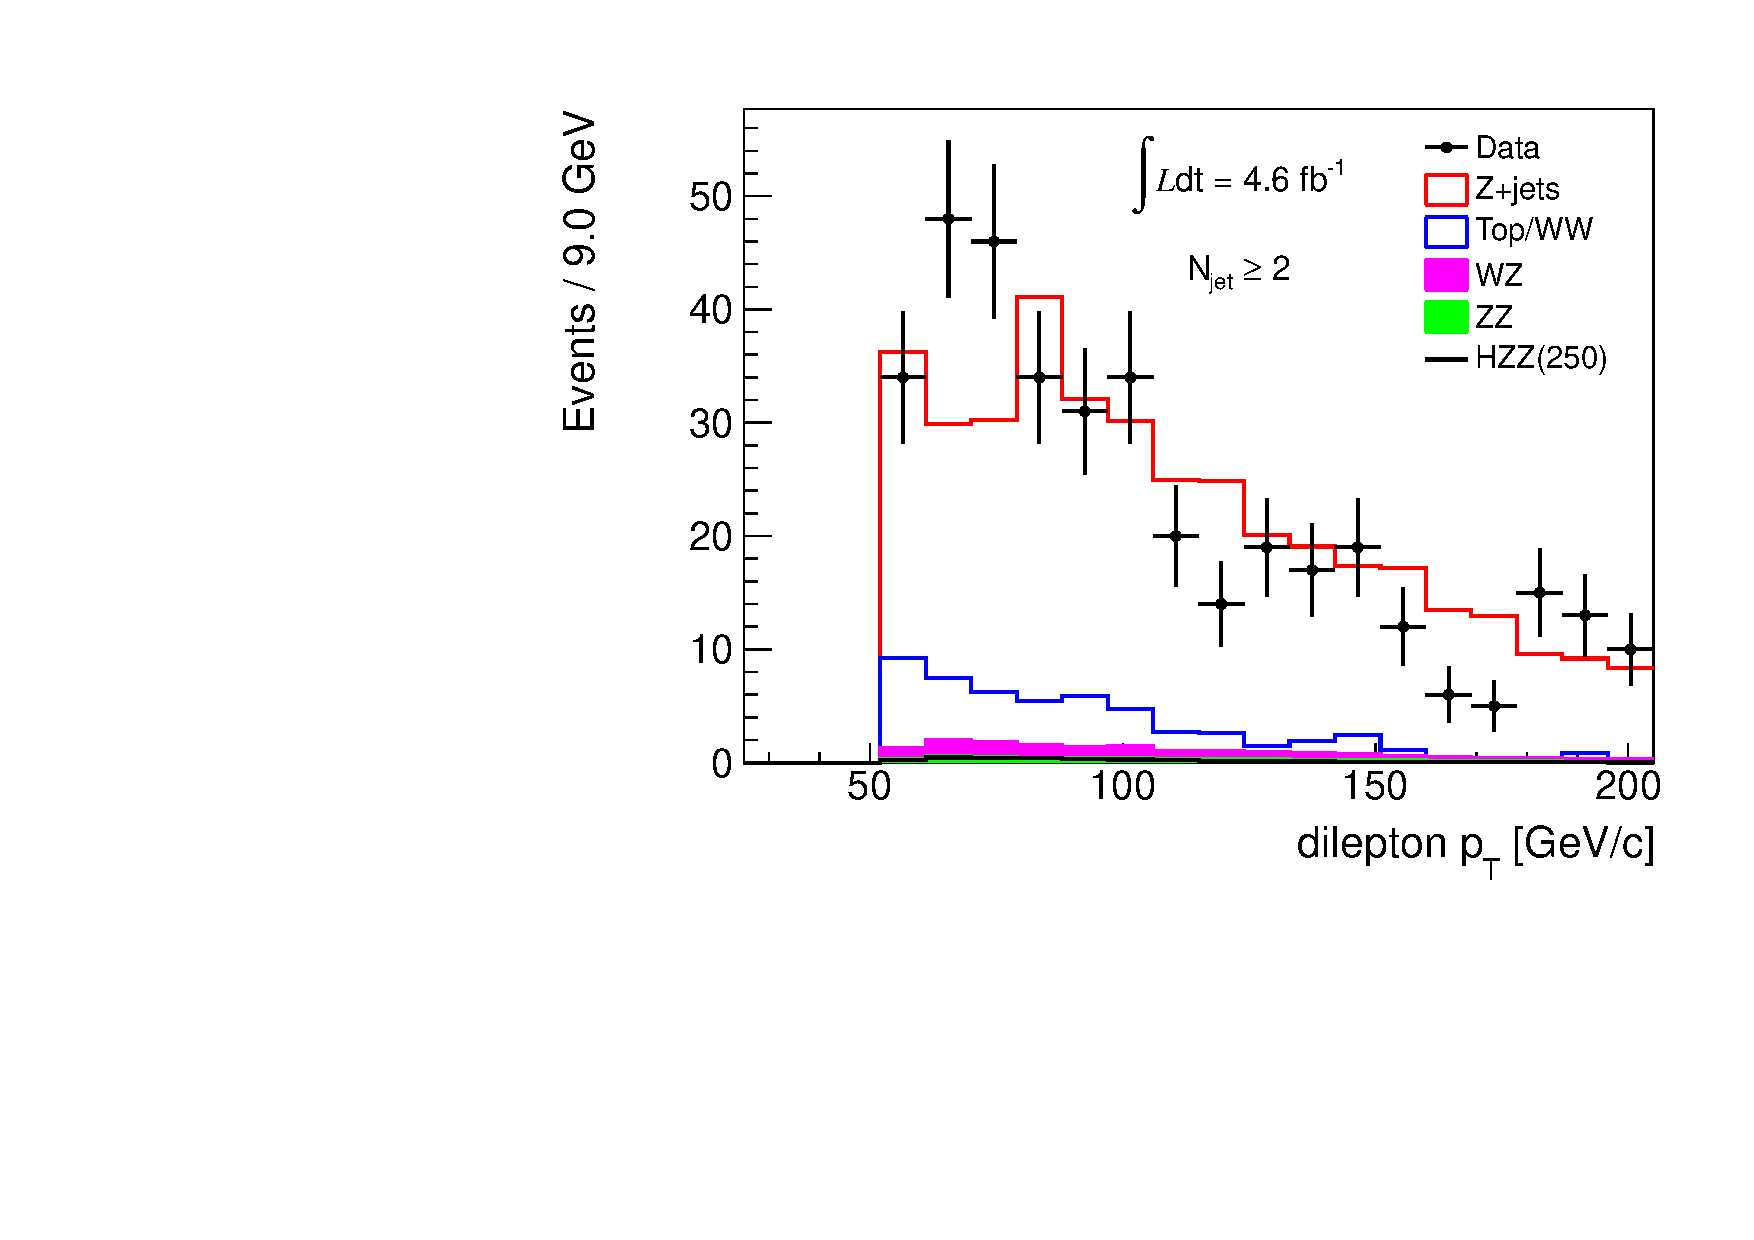
\includegraphics[width=.4\textwidth]{figures/presel_mH250_mm_dileppt_2j.pdf}}
\caption{Dilepton $p_T$ distribution in the muon channel after the $\ZZ$ preselection observed in data corresponding to $2.1$~\ifb data in 
the Inclusive~\subref{subfig:zpt_mm_incl}, 0-Jet~\subref{subfig:zpt_mm_0j}, 1-Jet~\subref{subfig:zpt_mm_1j} and 2-Jet~\subref{subfig:zpt_mm_2j} bins, 
compared to the expected from simulation for signal and background. The MC backgrounds are scaled as appropriate and the photon+jets estimate of the 
Z+jets background is added to the stack.}
\label{fig:zpt_zzpresel_mm}
\end{center}
\end{figure}
%%%%%%%%

%%%%%%%%
\begin{figure}[!hbtp]
\begin{center}
\subfigure[Inclusive]{\label{subfig:zpt_ee_incl}
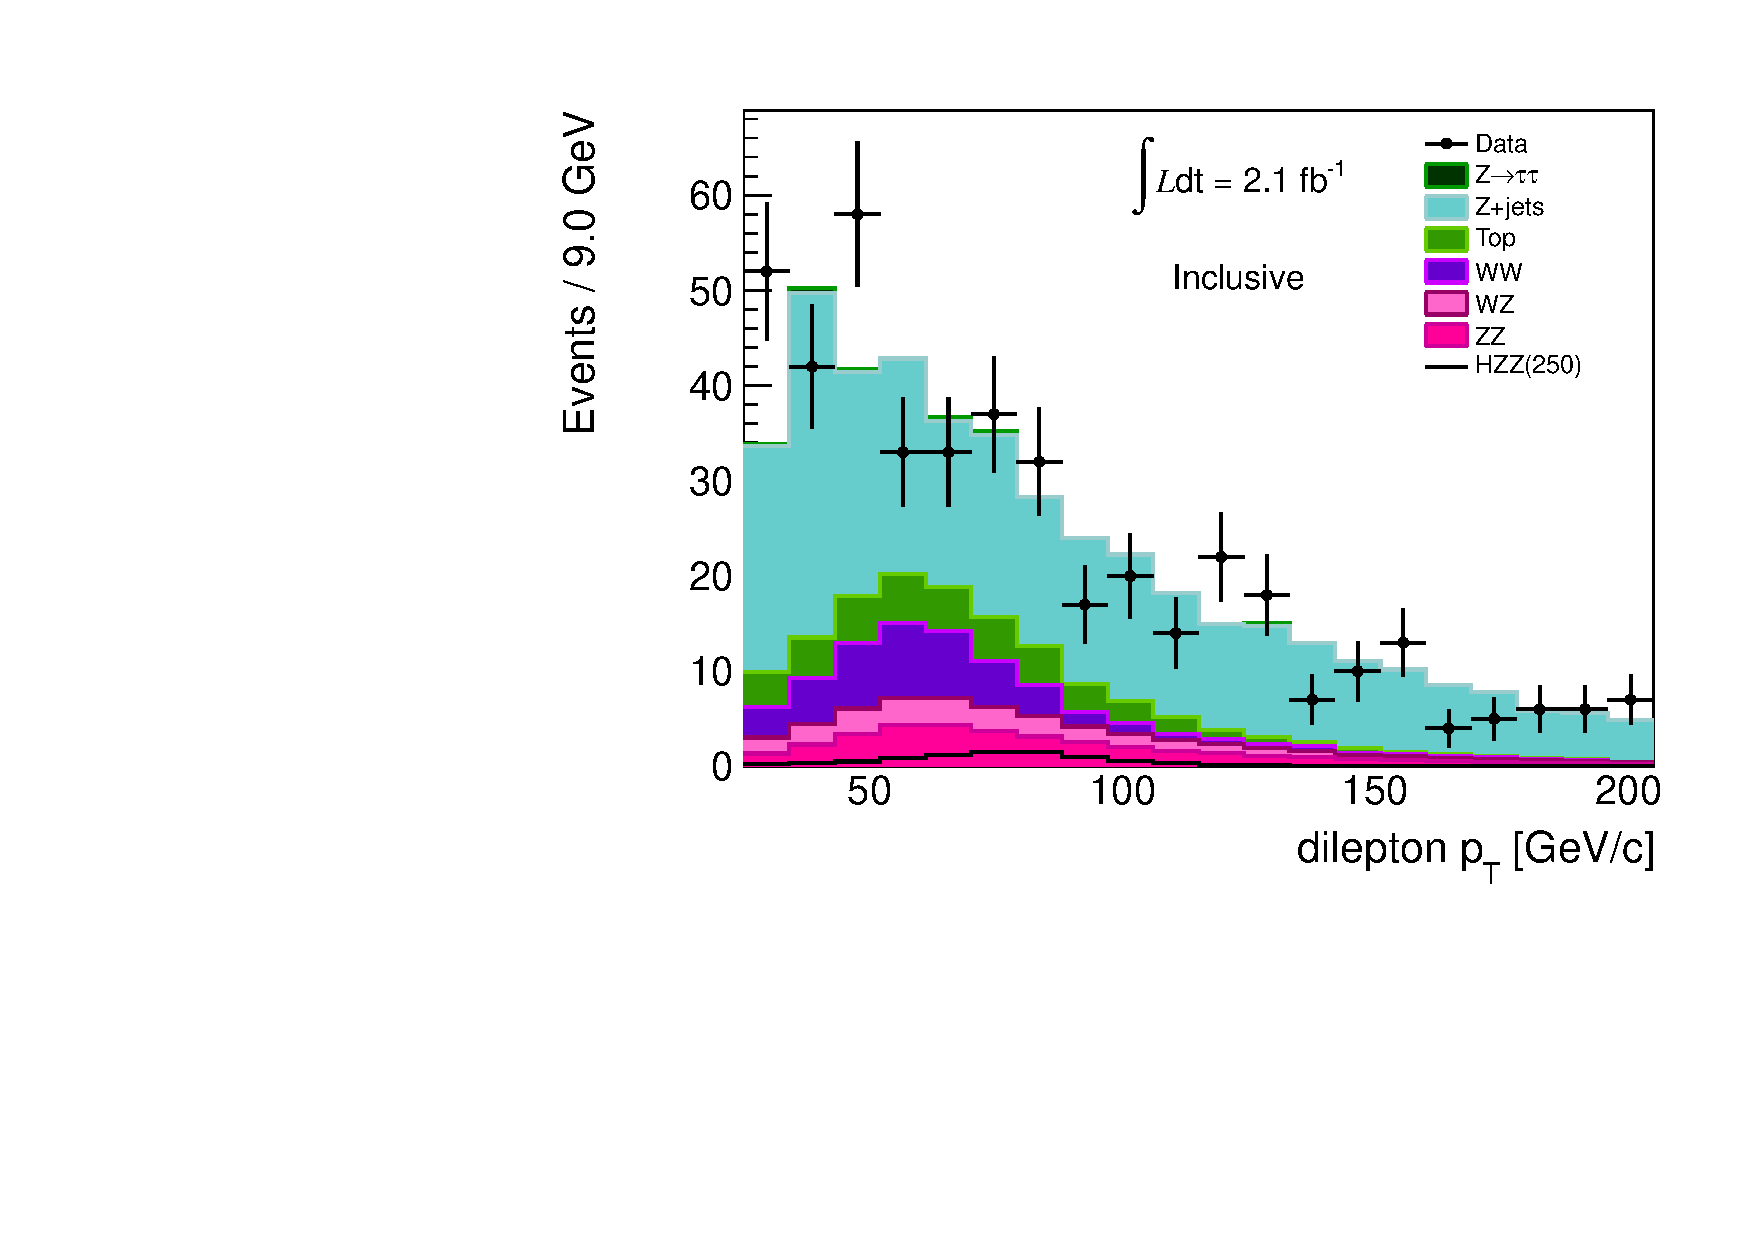
\includegraphics[width=.4\textwidth]{figures/presel_mH250_ee_dileppt_incl.pdf}}
\subfigure[0-Jet]{\label{subfig:zpt_ee_0j}
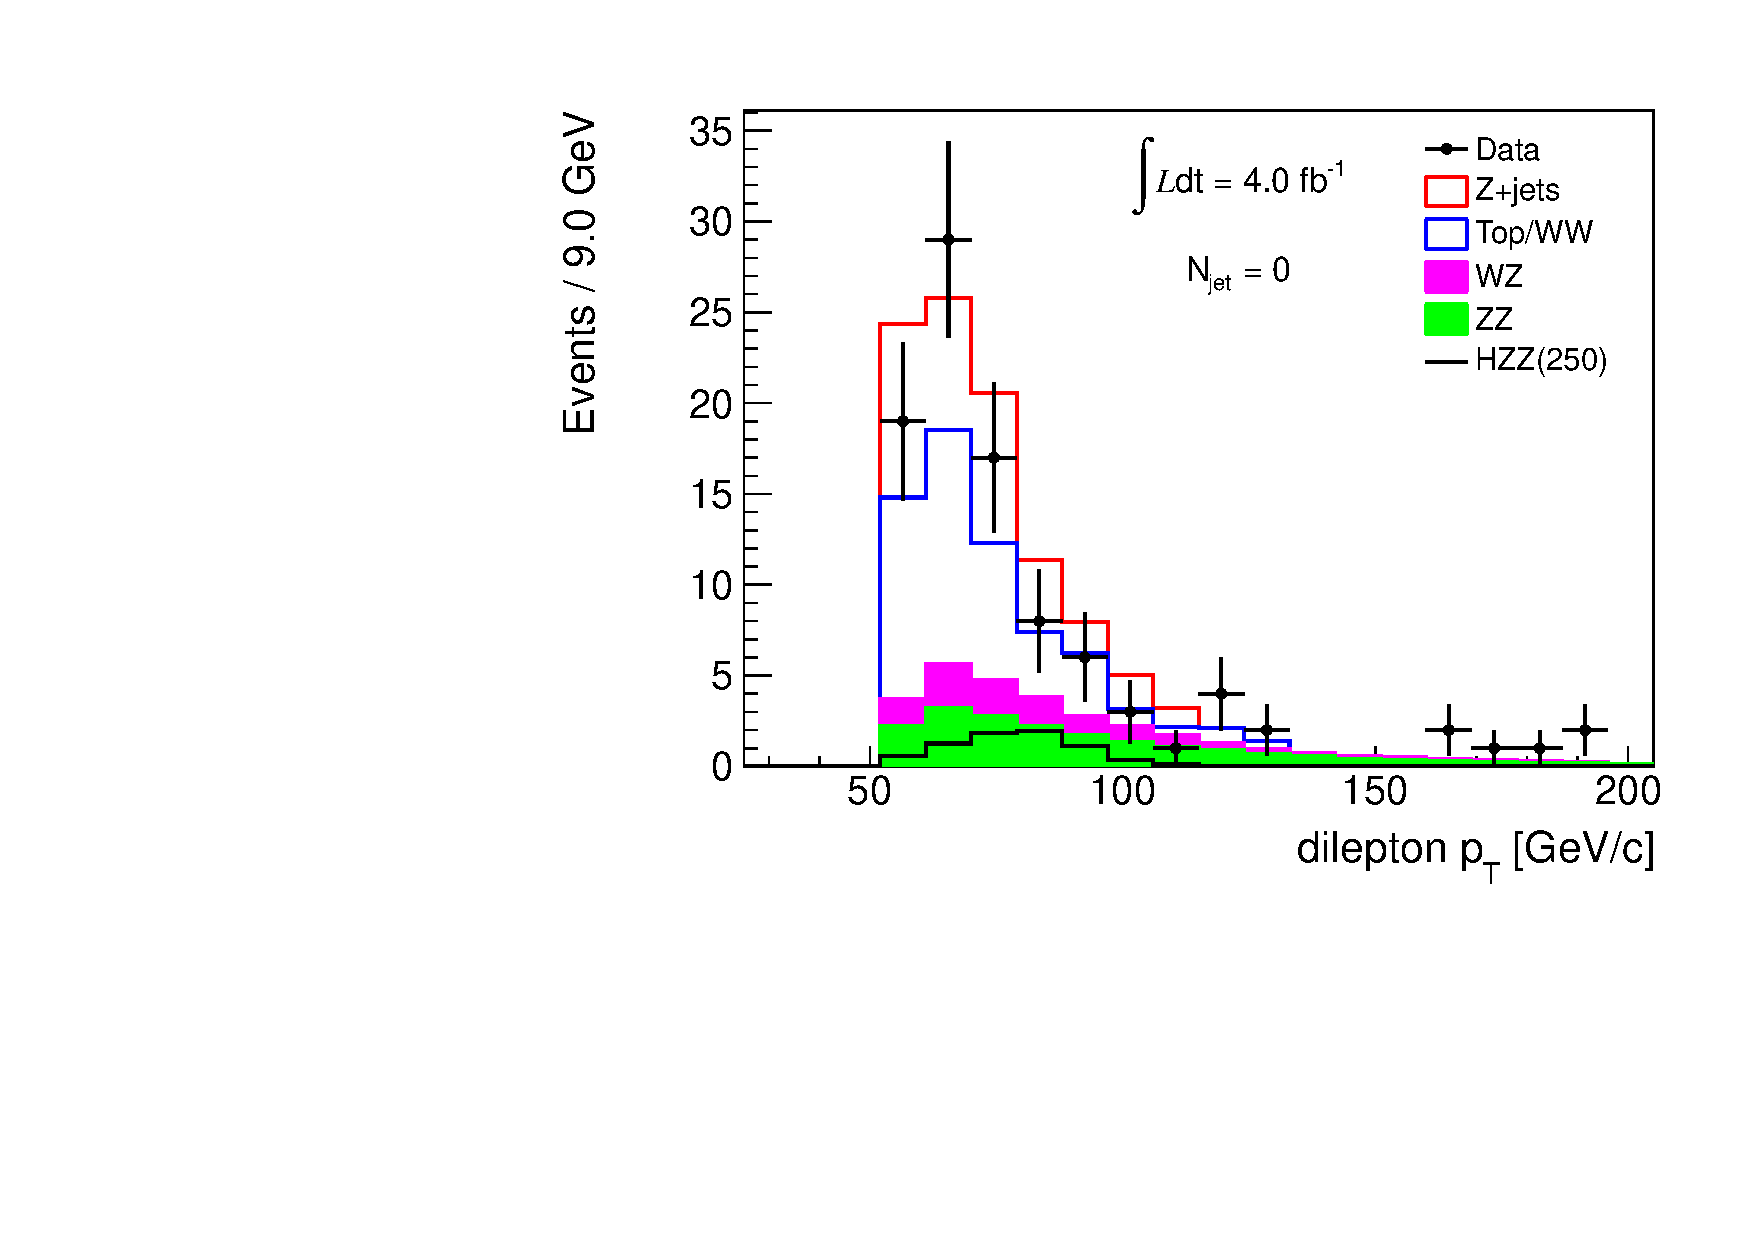
\includegraphics[width=.4\textwidth]{figures/presel_mH250_ee_dileppt_0j.pdf}} \\
\subfigure[1-Jet]{\label{subfig:zpt_ee_1j}
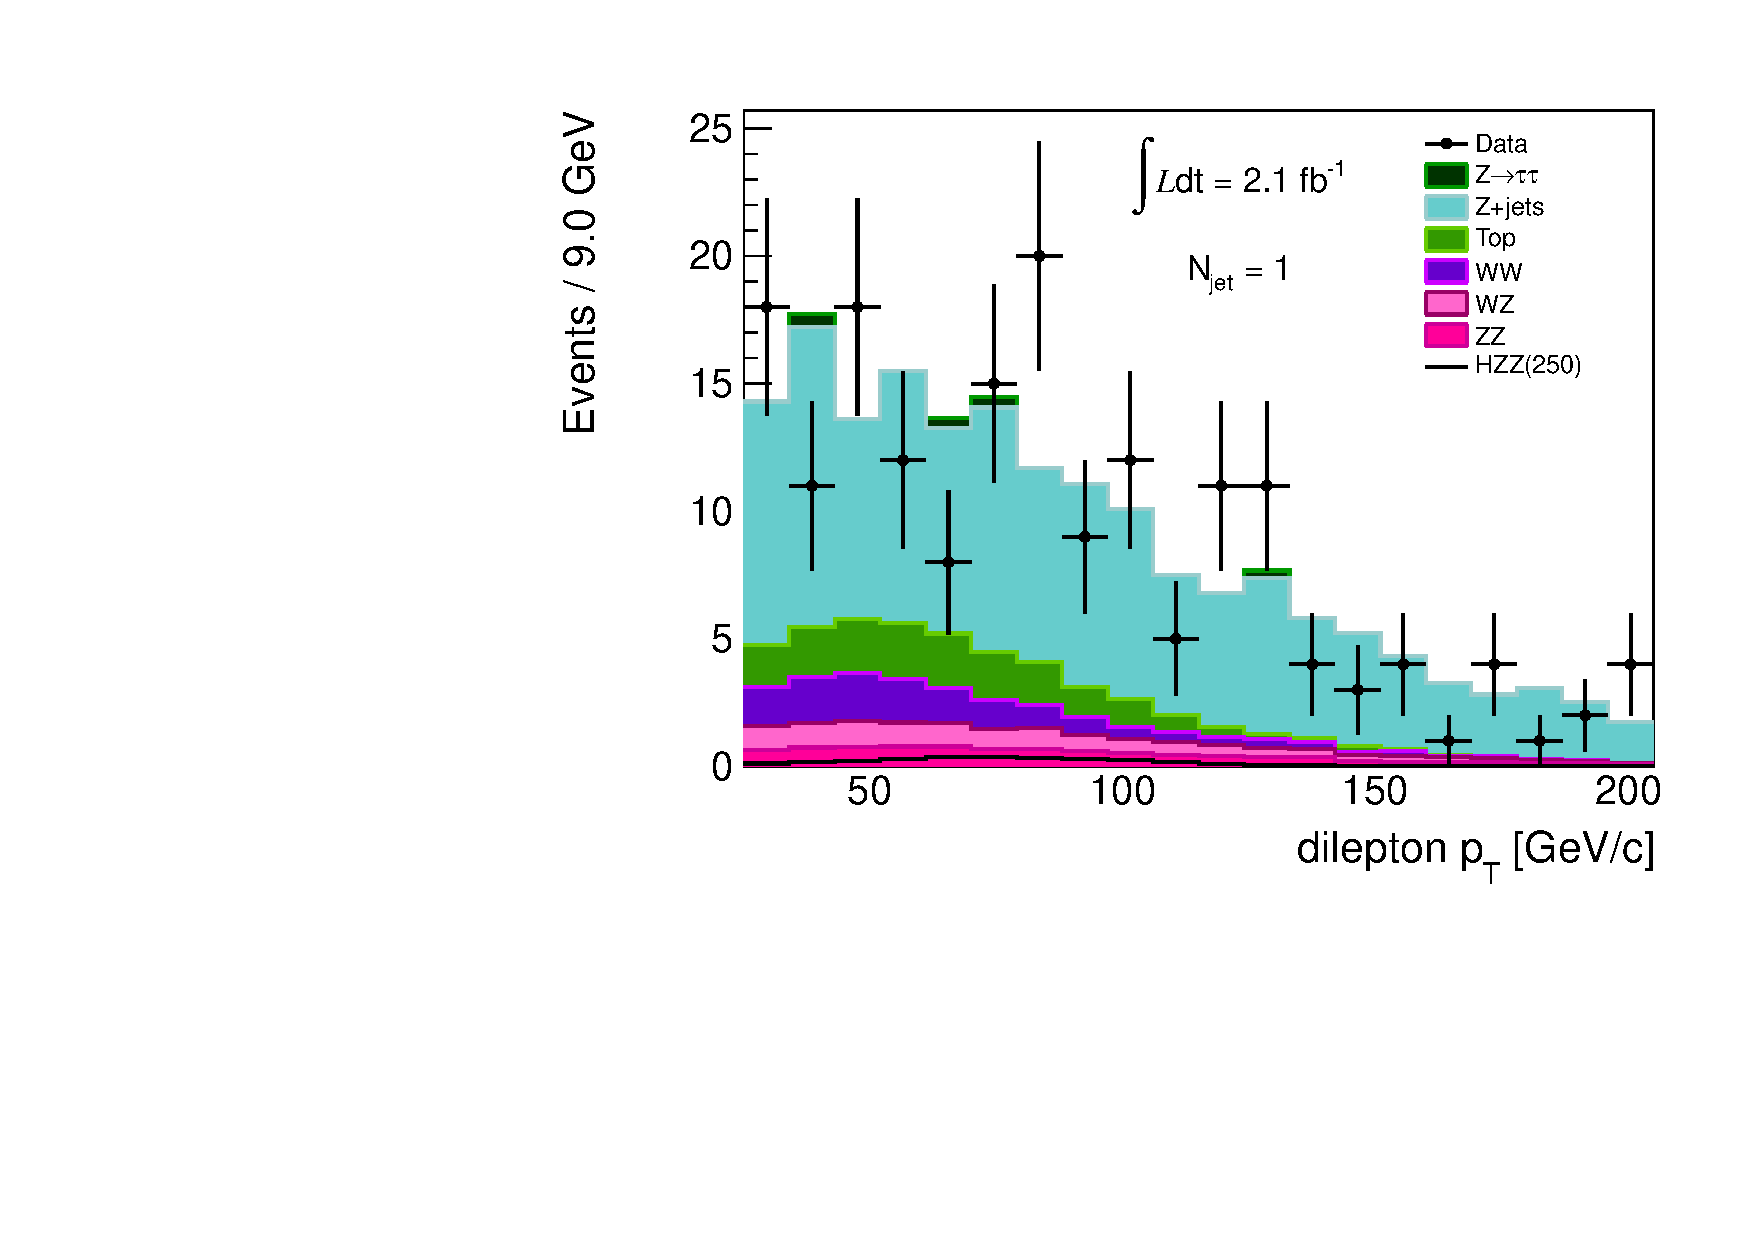
\includegraphics[width=.4\textwidth]{figures/presel_mH250_ee_dileppt_1j.pdf}}
\subfigure[$\geq$2 Jets]{\label{subfig:zpt_ee_2j}
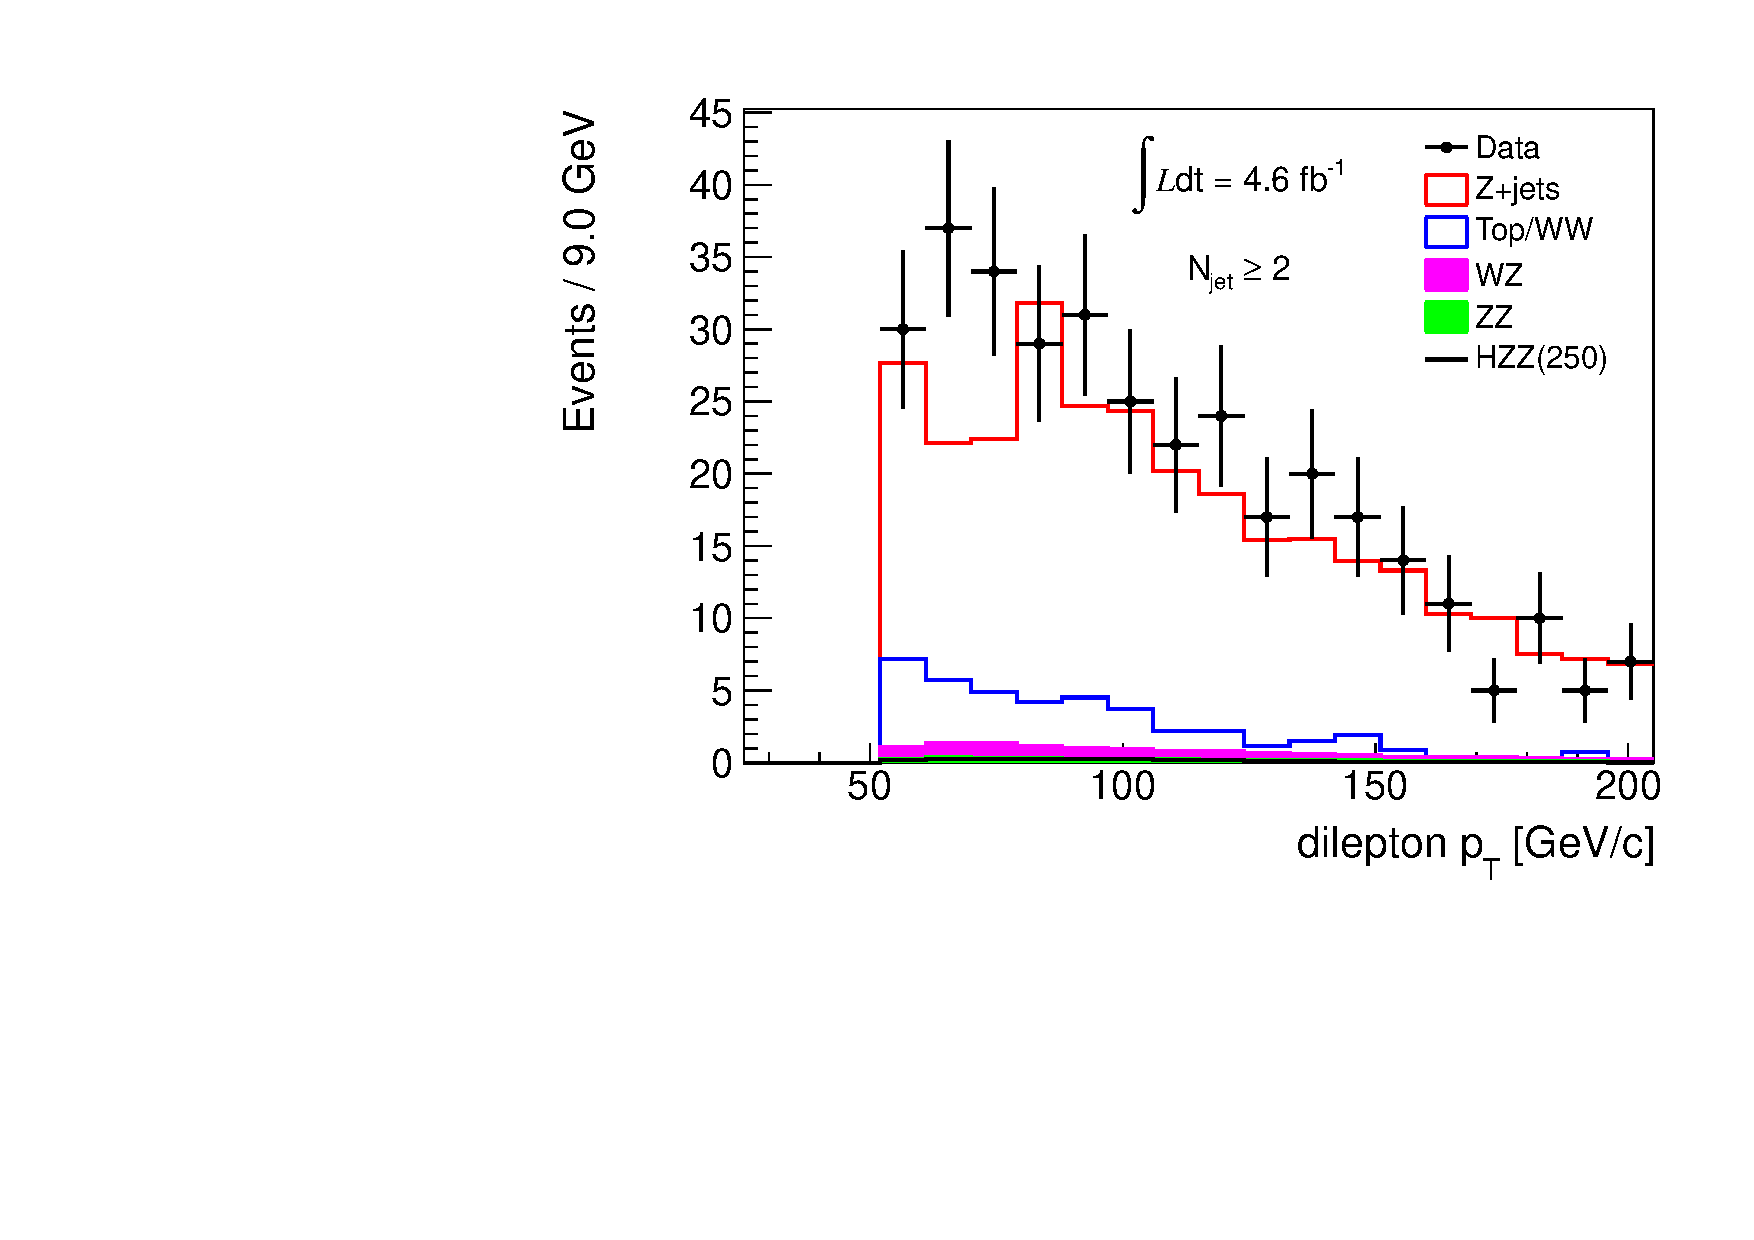
\includegraphics[width=.4\textwidth]{figures/presel_mH250_ee_dileppt_2j.pdf}}
\caption{Dilepton $p_T$ distribution in the electron channel after the $\ZZ$ preselection observed in data corresponding to $2.1$~\ifb data in 
the Inclusive~\subref{subfig:zpt_ee_incl}, 0-Jet~\subref{subfig:zpt_ee_0j}, 1-Jet~\subref{subfig:zpt_ee_1j} and 2-Jet~\subref{subfig:zpt_ee_2j} bins, 
compared to the expected from simulation for signal and background. The MC backgrounds are scaled as appropriate and the photon+jets estimate of the 
Z+jets background is added to the stack.}
\label{fig:zpt_zzpresel_ee}
\end{center}
\end{figure}
%%%%%%%%

%%%%%%%%
\begin{figure}[!hbtp]
\begin{center}
\subfigure[Inclusive]{\label{subfig:met_mm_incl}
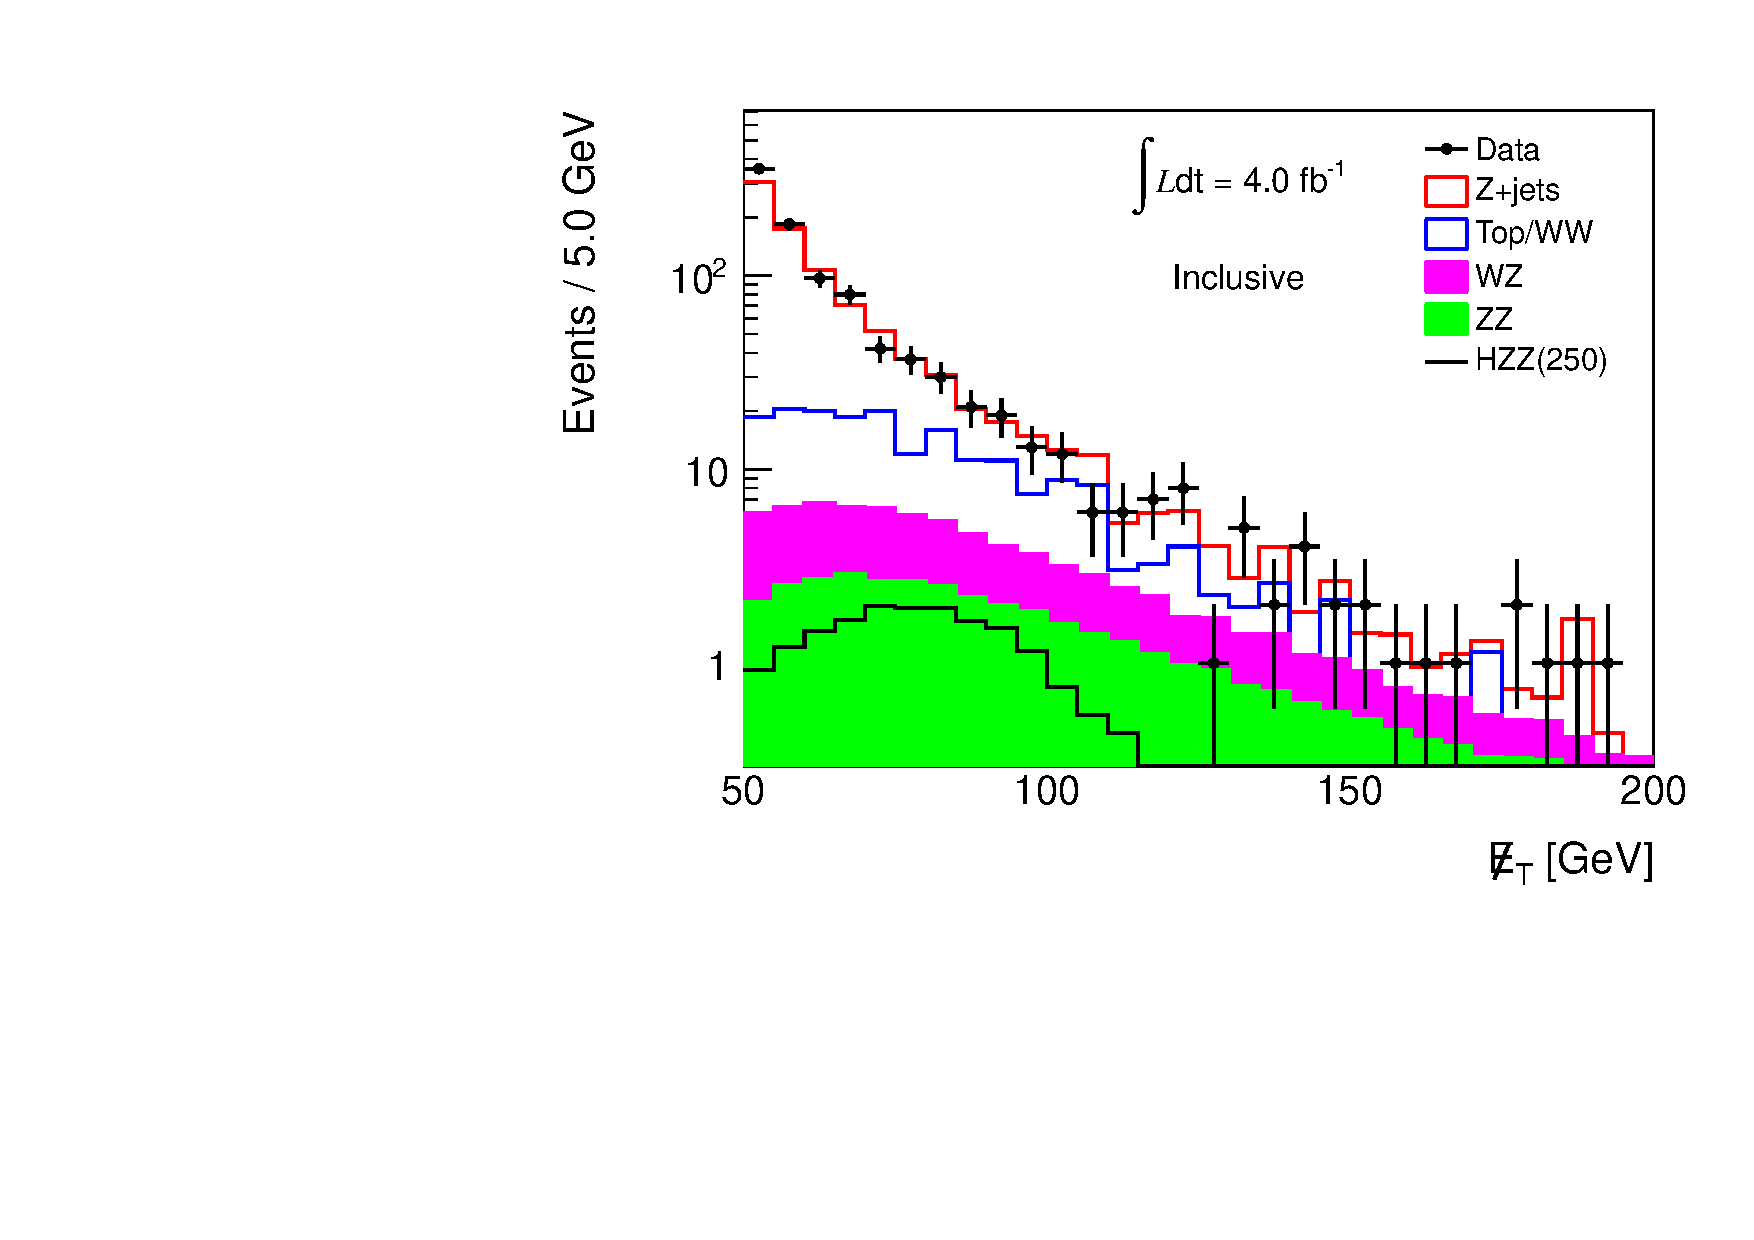
\includegraphics[width=.4\textwidth]{figures/presel_mH250_mm_metlog_incl.pdf}}
\subfigure[0-Jet]{\label{subfig:met_mm_0j}
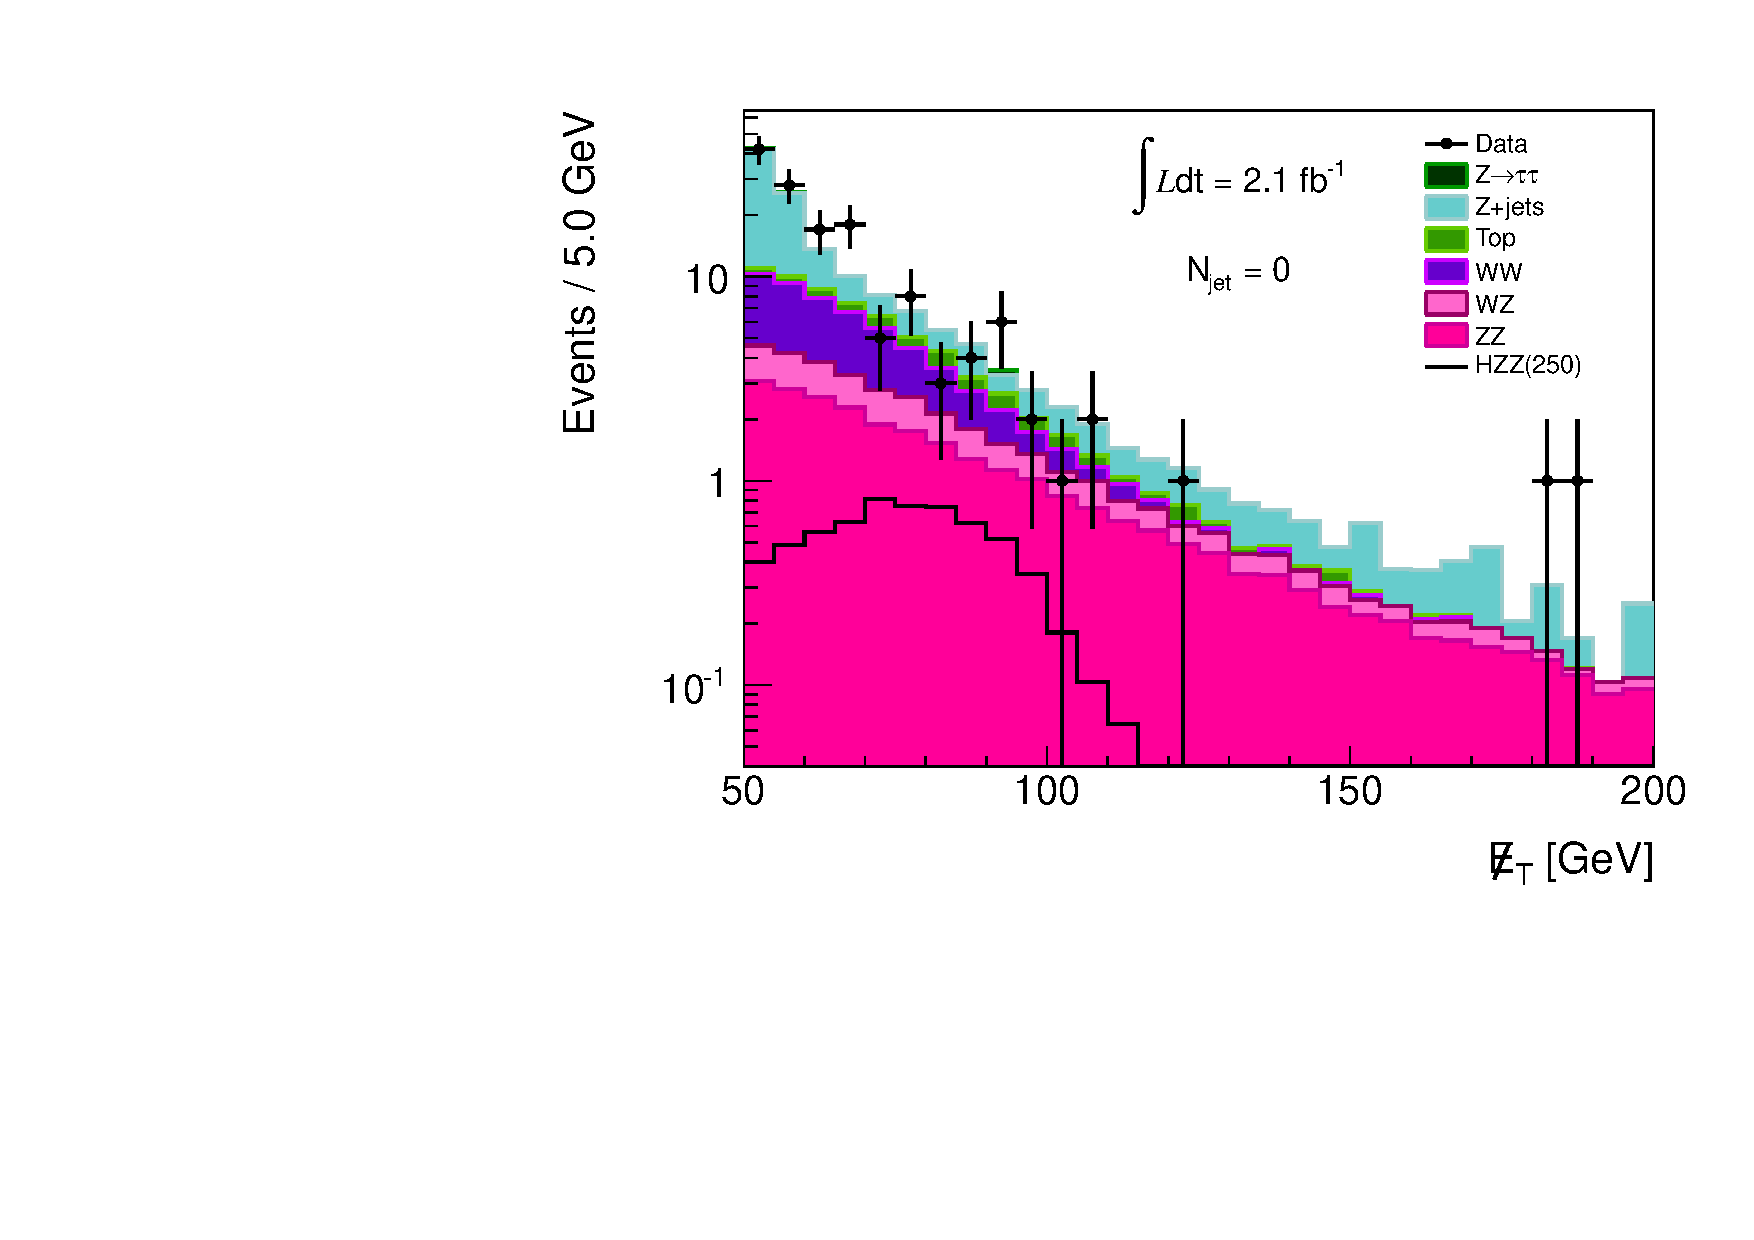
\includegraphics[width=.4\textwidth]{figures/presel_mH250_mm_metlog_0j.pdf}} \\
\subfigure[1-Jet]{\label{subfig:met_mm_1j}
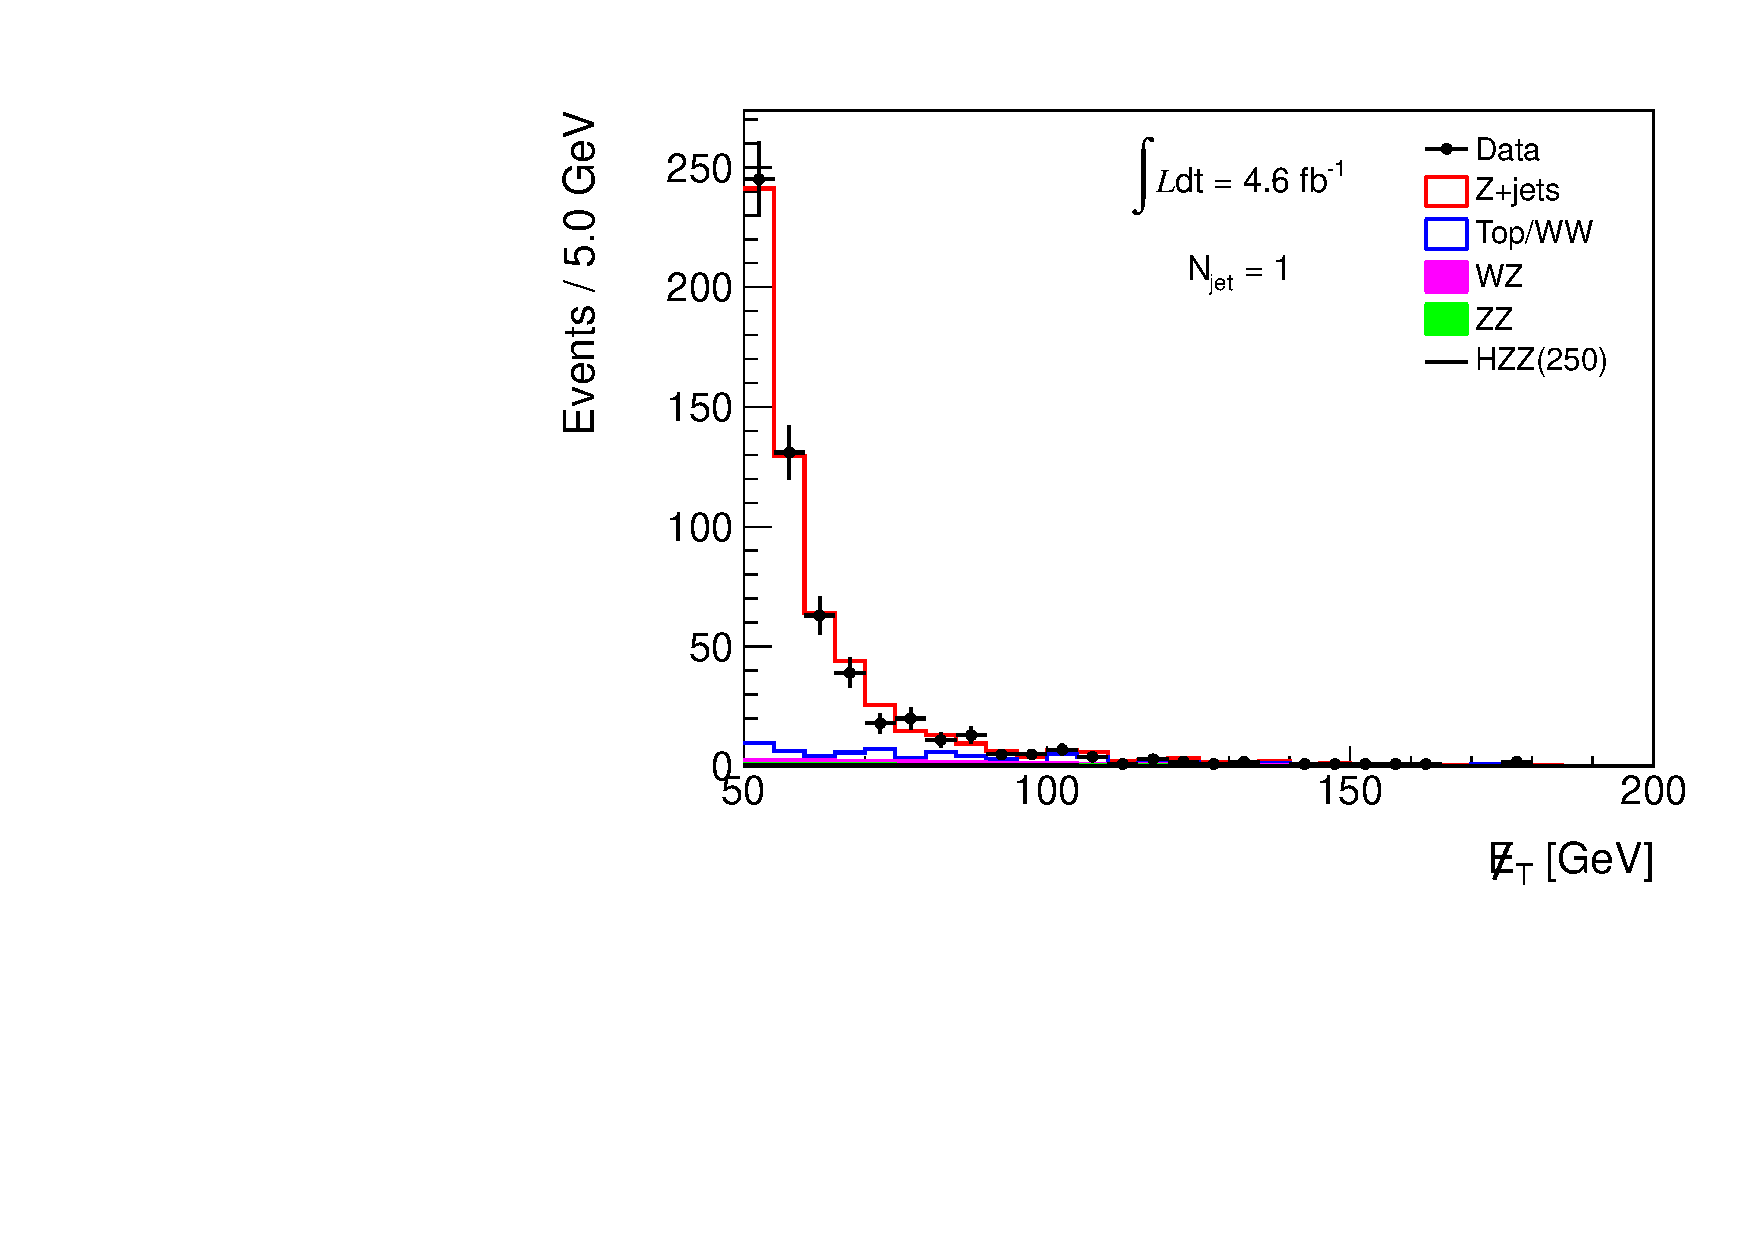
\includegraphics[width=.4\textwidth]{figures/presel_mH250_mm_metlog_1j.pdf}}
\subfigure[$\geq$2 Jets]{\label{subfig:met_mm_2j}
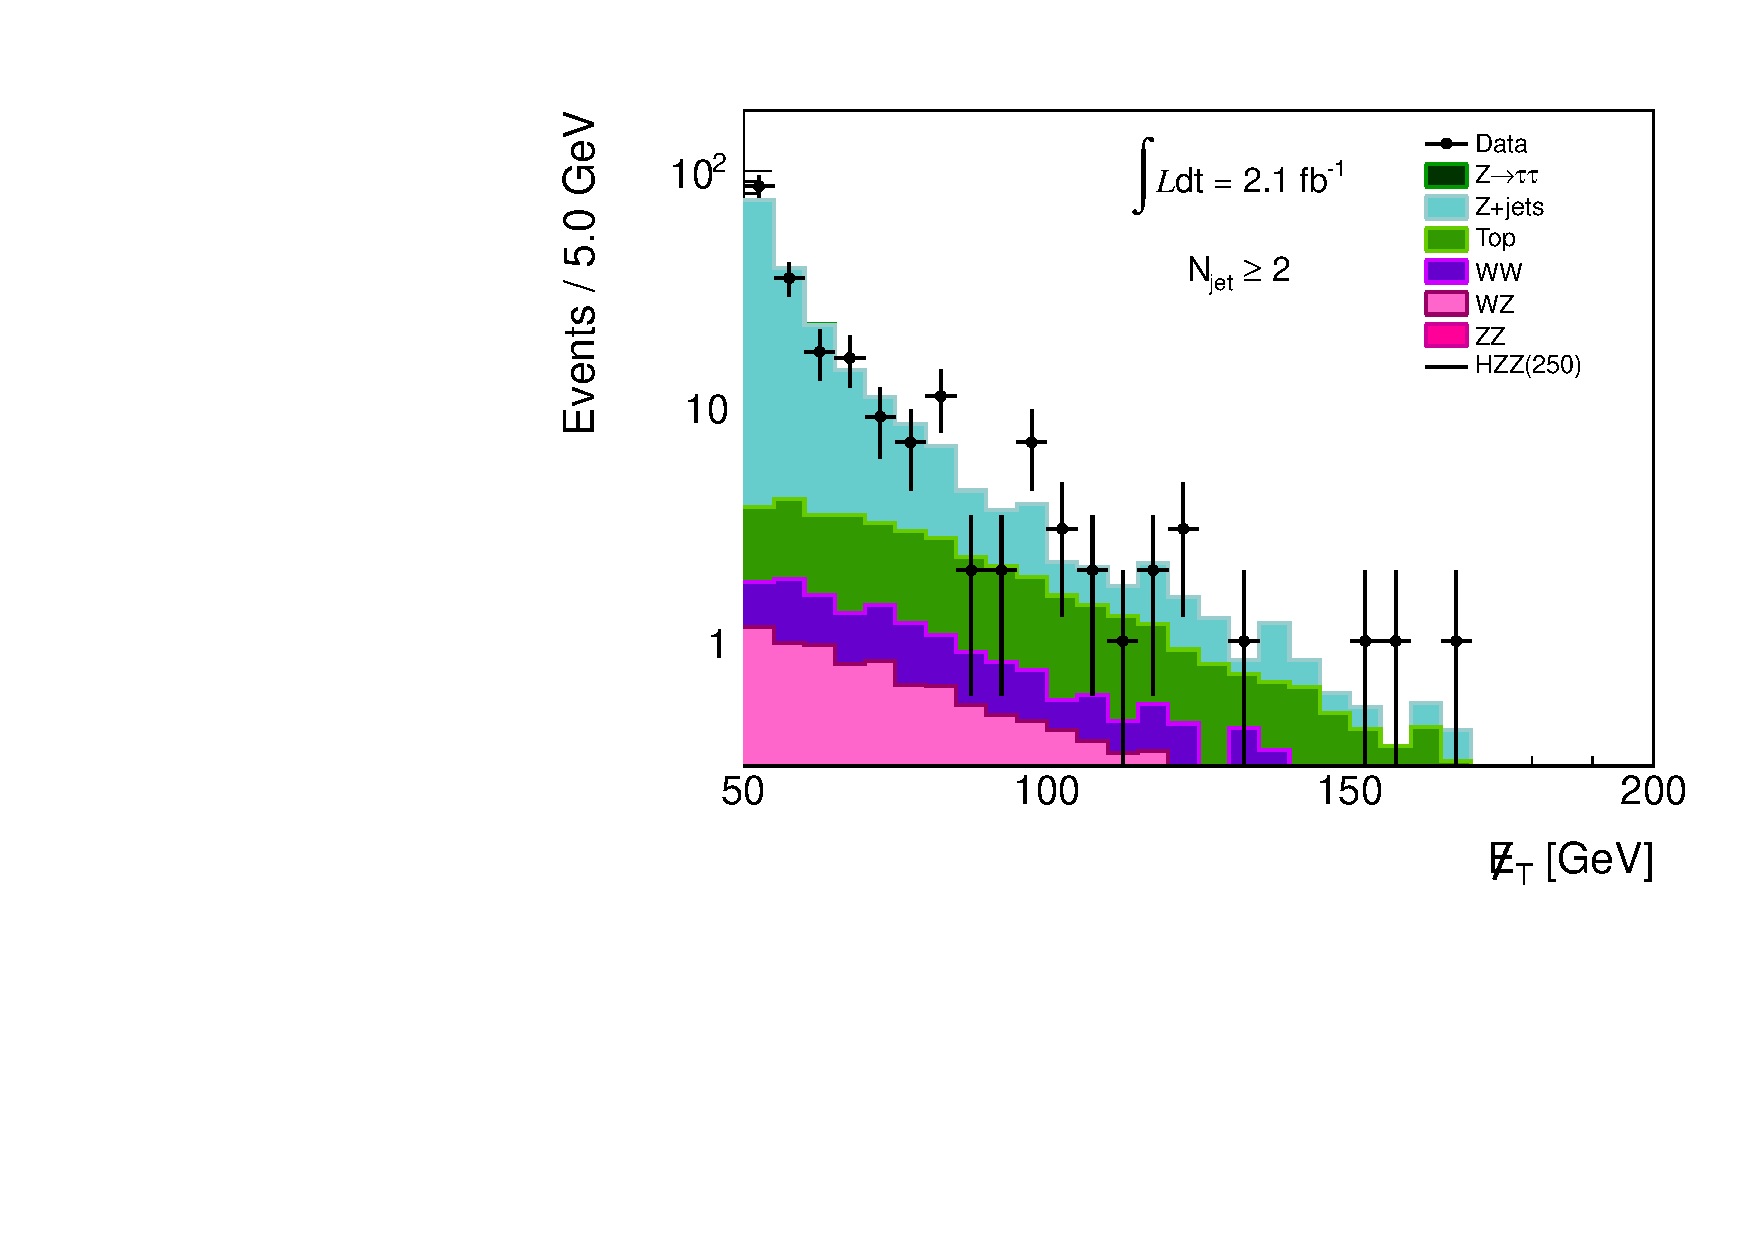
\includegraphics[width=.4\textwidth]{figures/presel_mH250_mm_metlog_2j.pdf}}
\caption{Missing transverse energy distribution in the muon channel after the $\ZZ$ preselection observed in data corresponding to $2.1$~\ifb data in 
the Inclusive~\subref{subfig:met_mm_incl}, 0-Jet~\subref{subfig:met_mm_0j}, 1-Jet~\subref{subfig:met_mm_1j} and 2-Jet~\subref{subfig:met_mm_2j} bins, 
compared to the expected from simulation for signal and background. The MC backgrounds are scaled as appropriate and the photon+jets estimate of the 
Z+jets background is added to the stack.}
\label{fig:met_zzpresel_mm}
\end{center}
\end{figure}
%%%%%%%%

%%%%%%%%
\begin{figure}[!hbtp]
\begin{center}
\subfigure[Inclusive]{\label{subfig:met_ee_incl}
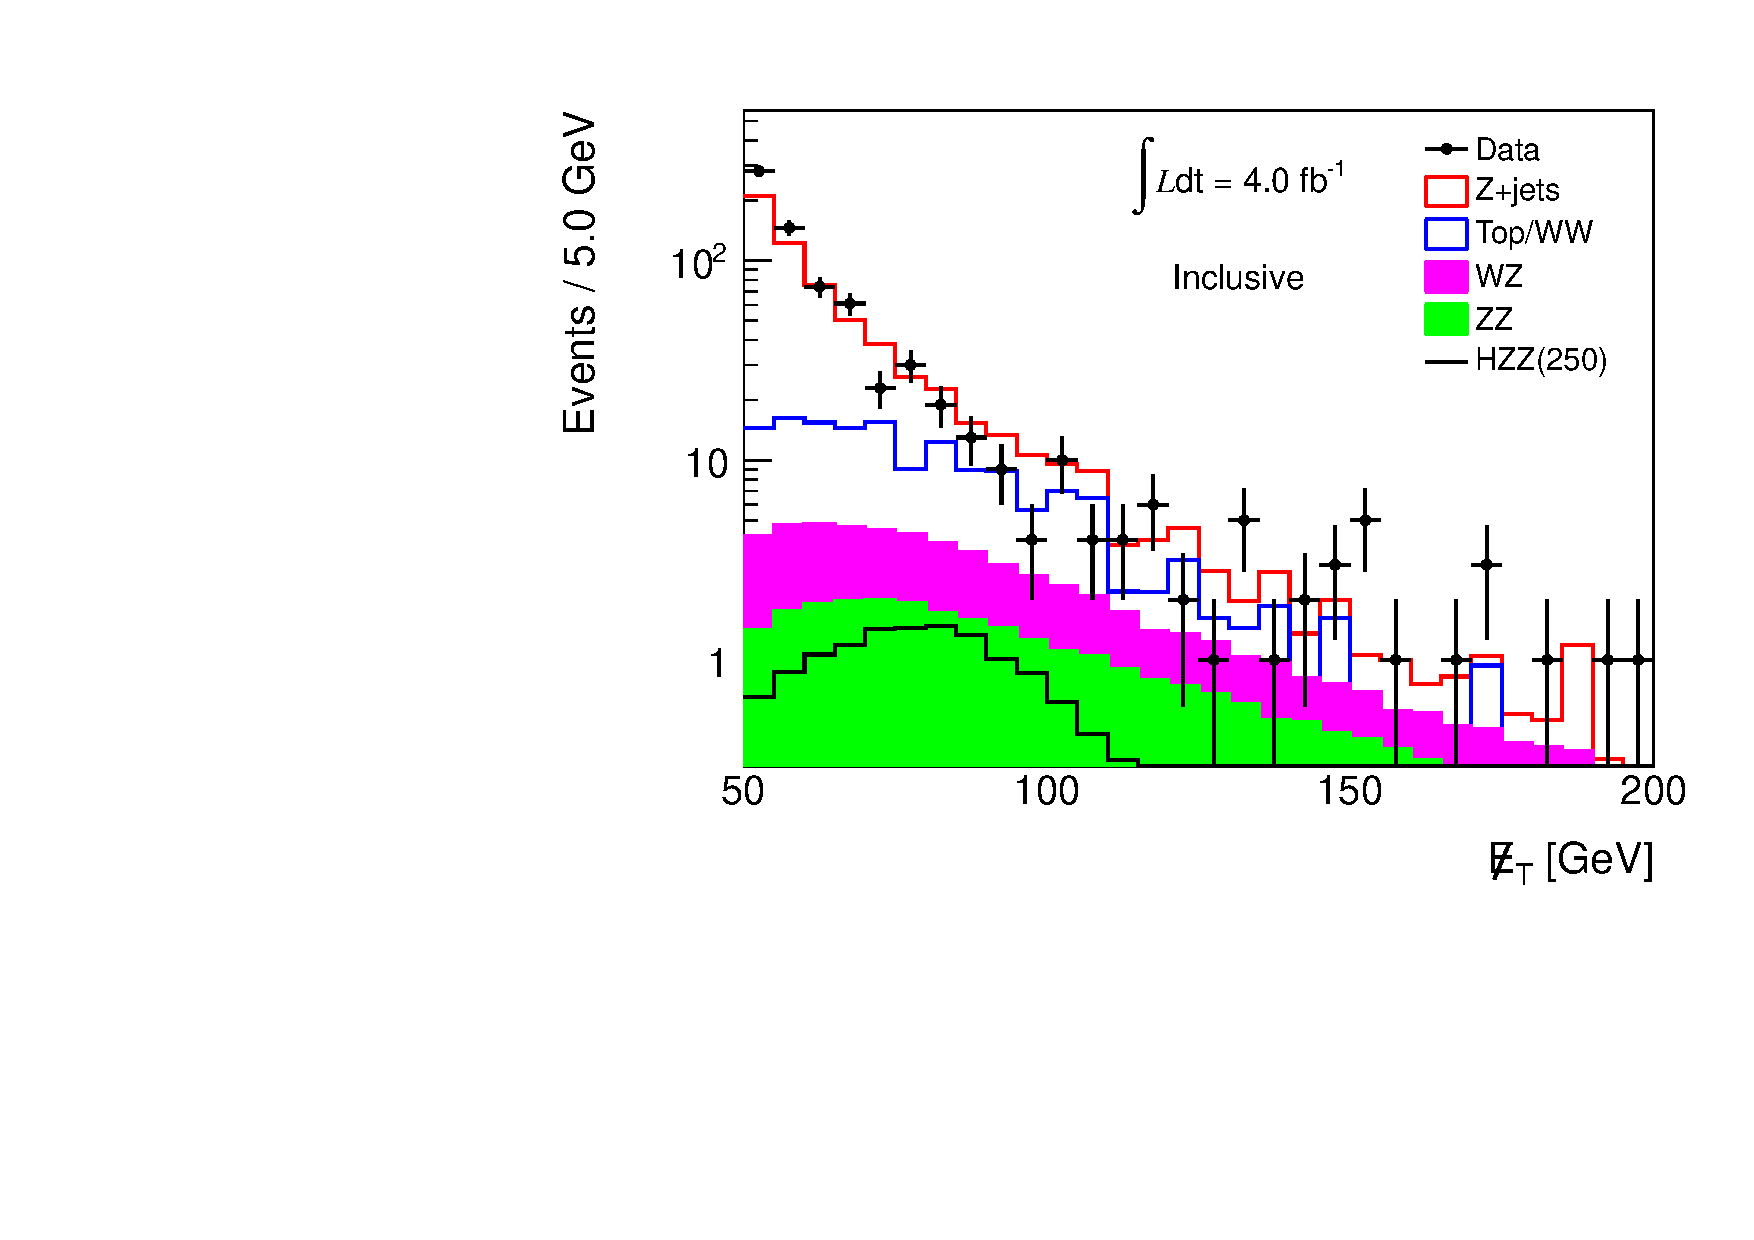
\includegraphics[width=.4\textwidth]{figures/presel_mH250_ee_metlog_incl.pdf}}
\subfigure[0-Jet]{\label{subfig:met_ee_0j}
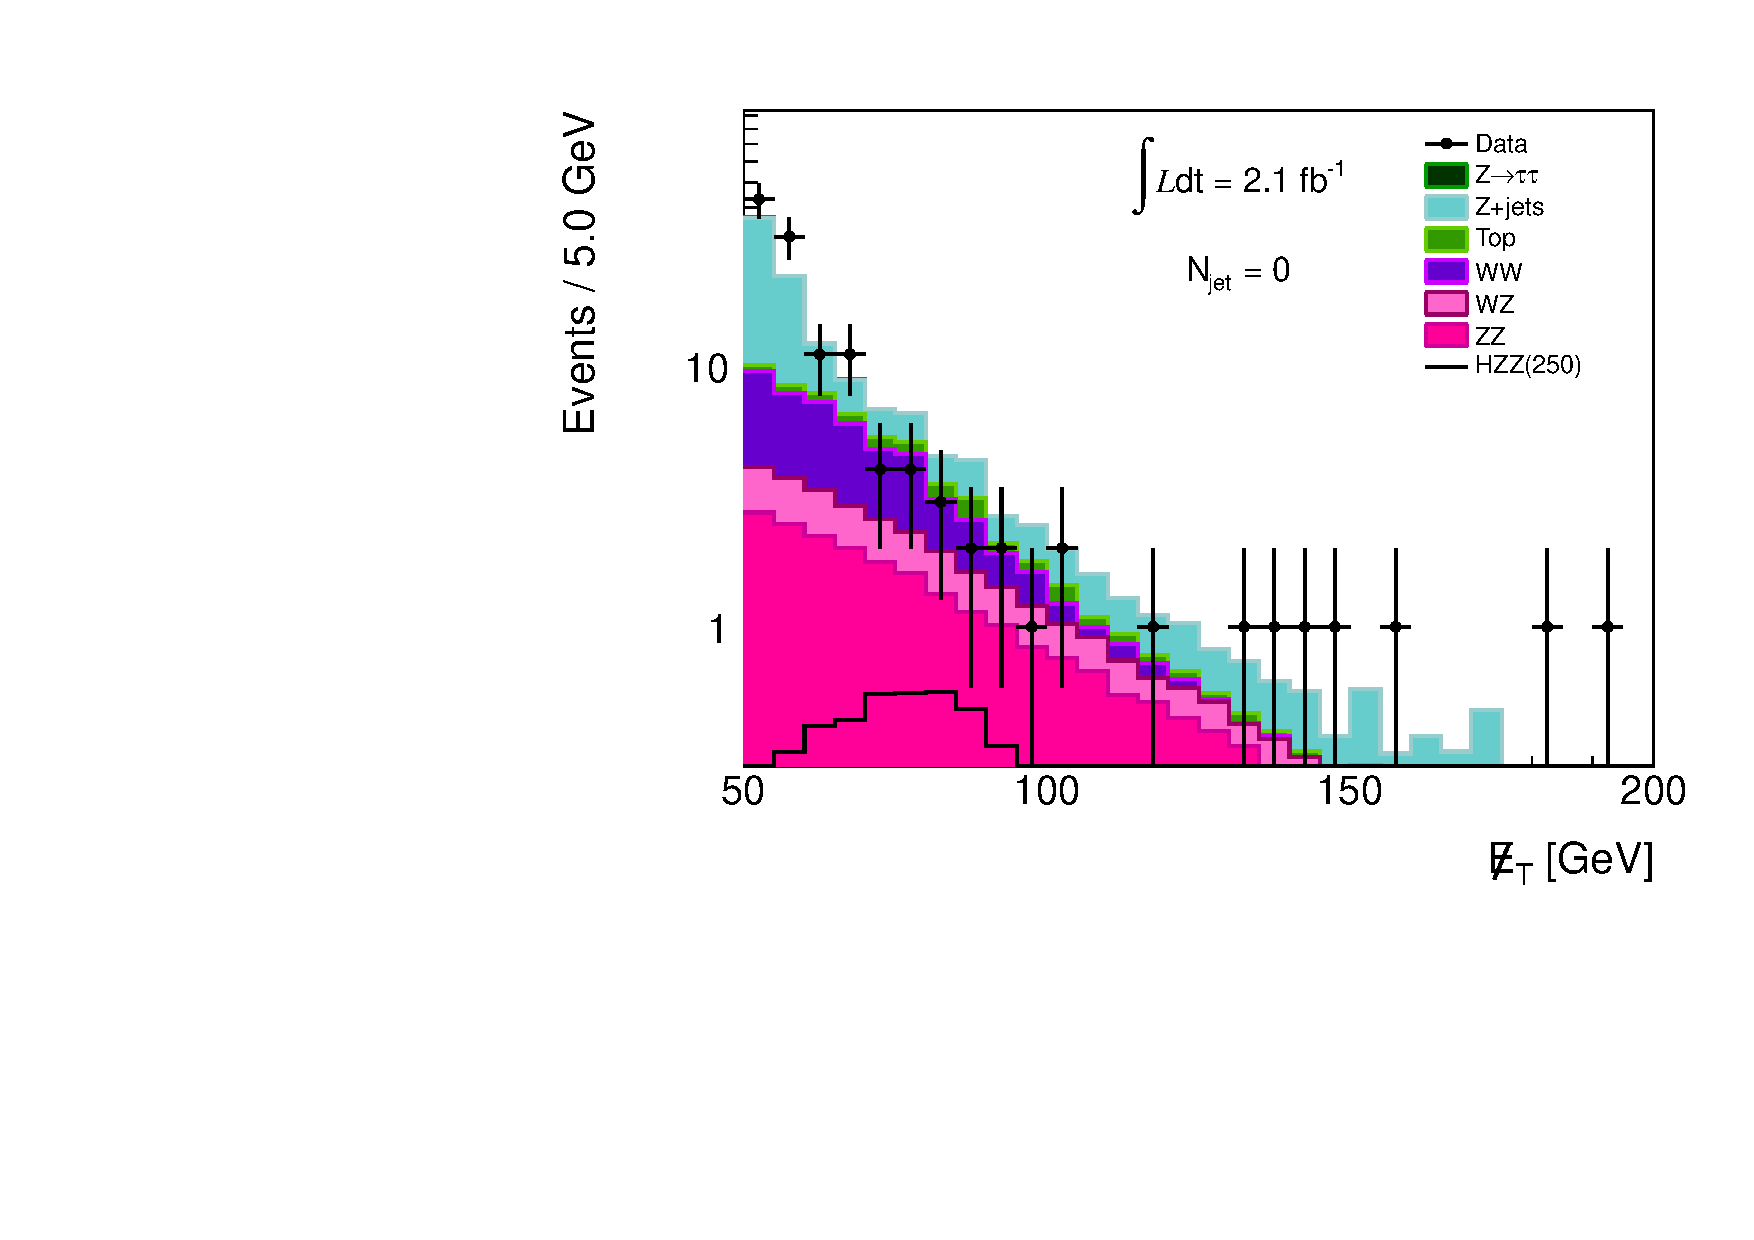
\includegraphics[width=.4\textwidth]{figures/presel_mH250_ee_metlog_0j.pdf}} \\
\subfigure[1-Jet]{\label{subfig:met_ee_1j}
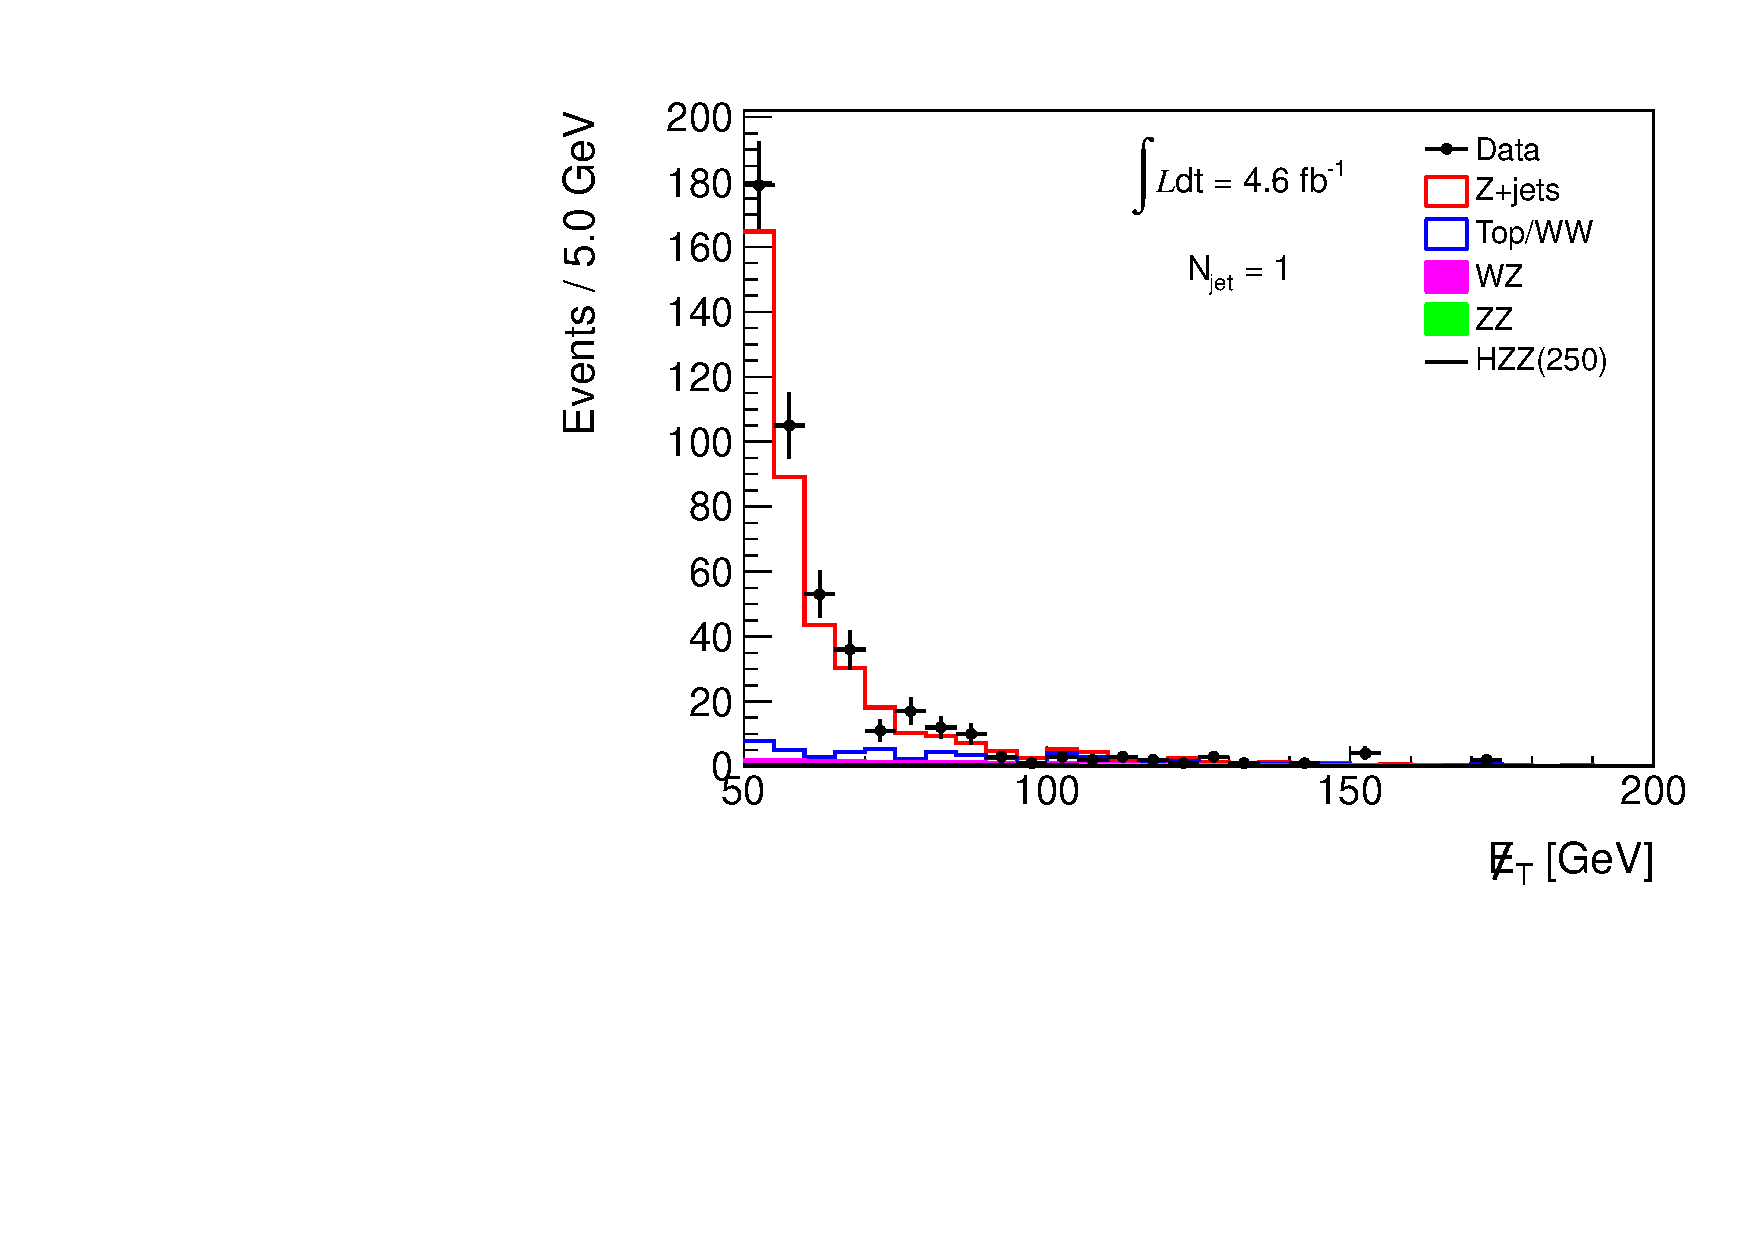
\includegraphics[width=.4\textwidth]{figures/presel_mH250_ee_metlog_1j.pdf}}
\subfigure[$\geq$2 Jets]{\label{subfig:met_ee_2j}
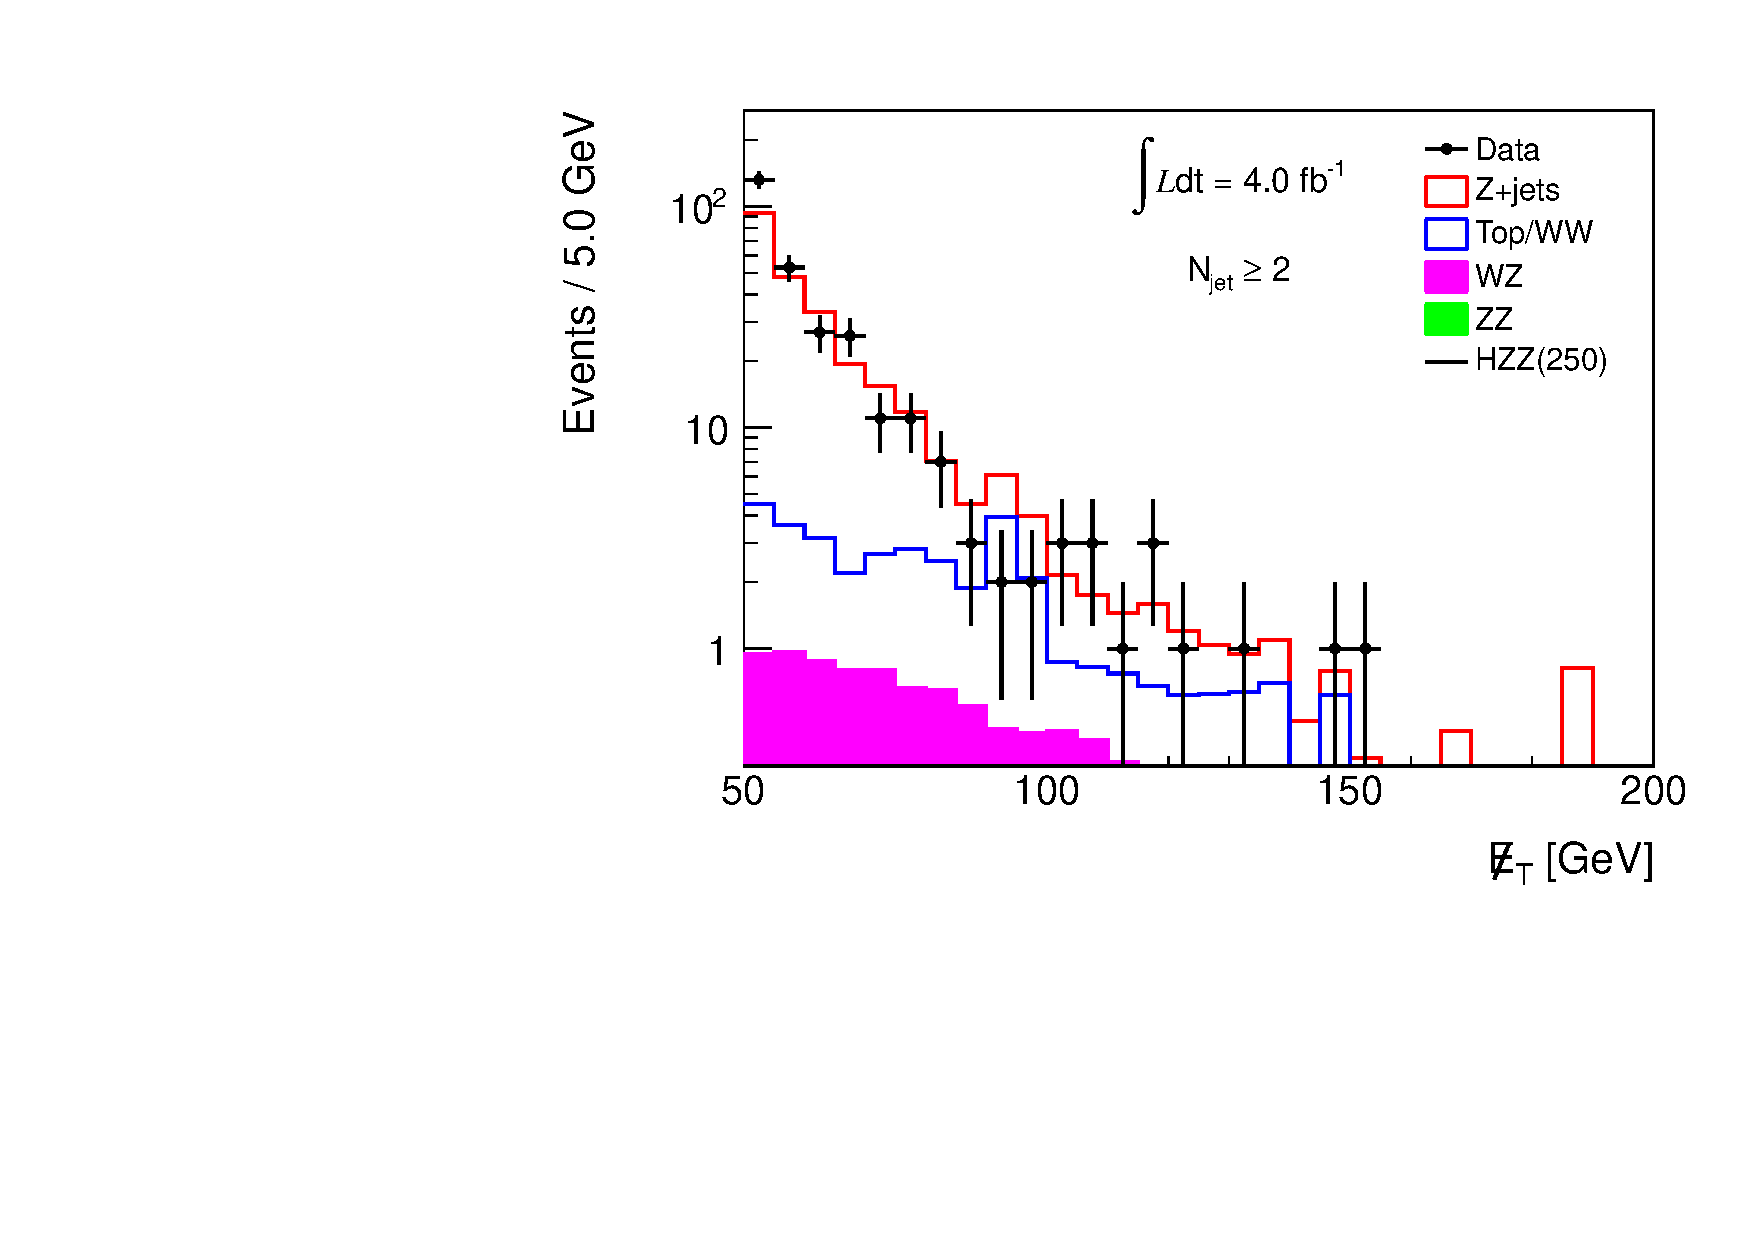
\includegraphics[width=.4\textwidth]{figures/presel_mH250_ee_metlog_2j.pdf}}
\caption{Missing transverse energy distribution in the electron channel after the $\ZZ$ preselection observed in data corresponding to $2.1$~\ifb data in 
the Inclusive~\subref{subfig:met_ee_incl}, 0-Jet~\subref{subfig:met_ee_0j}, 1-Jet~\subref{subfig:met_ee_1j} and 2-Jet~\subref{subfig:met_ee_2j} bins, 
compared to the expected from simulation for signal and background. The MC backgrounds are scaled as appropriate and the photon+jets estimate of the 
Z+jets background is added to the stack.}
\label{fig:met_zzpresel_ee}
\end{center}
\end{figure}
%%%%%%%%

%%%%%%%%
\begin{figure}[!hbtp]
\begin{center}
\subfigure[Inclusive]{\label{subfig:mt_mm_incl}
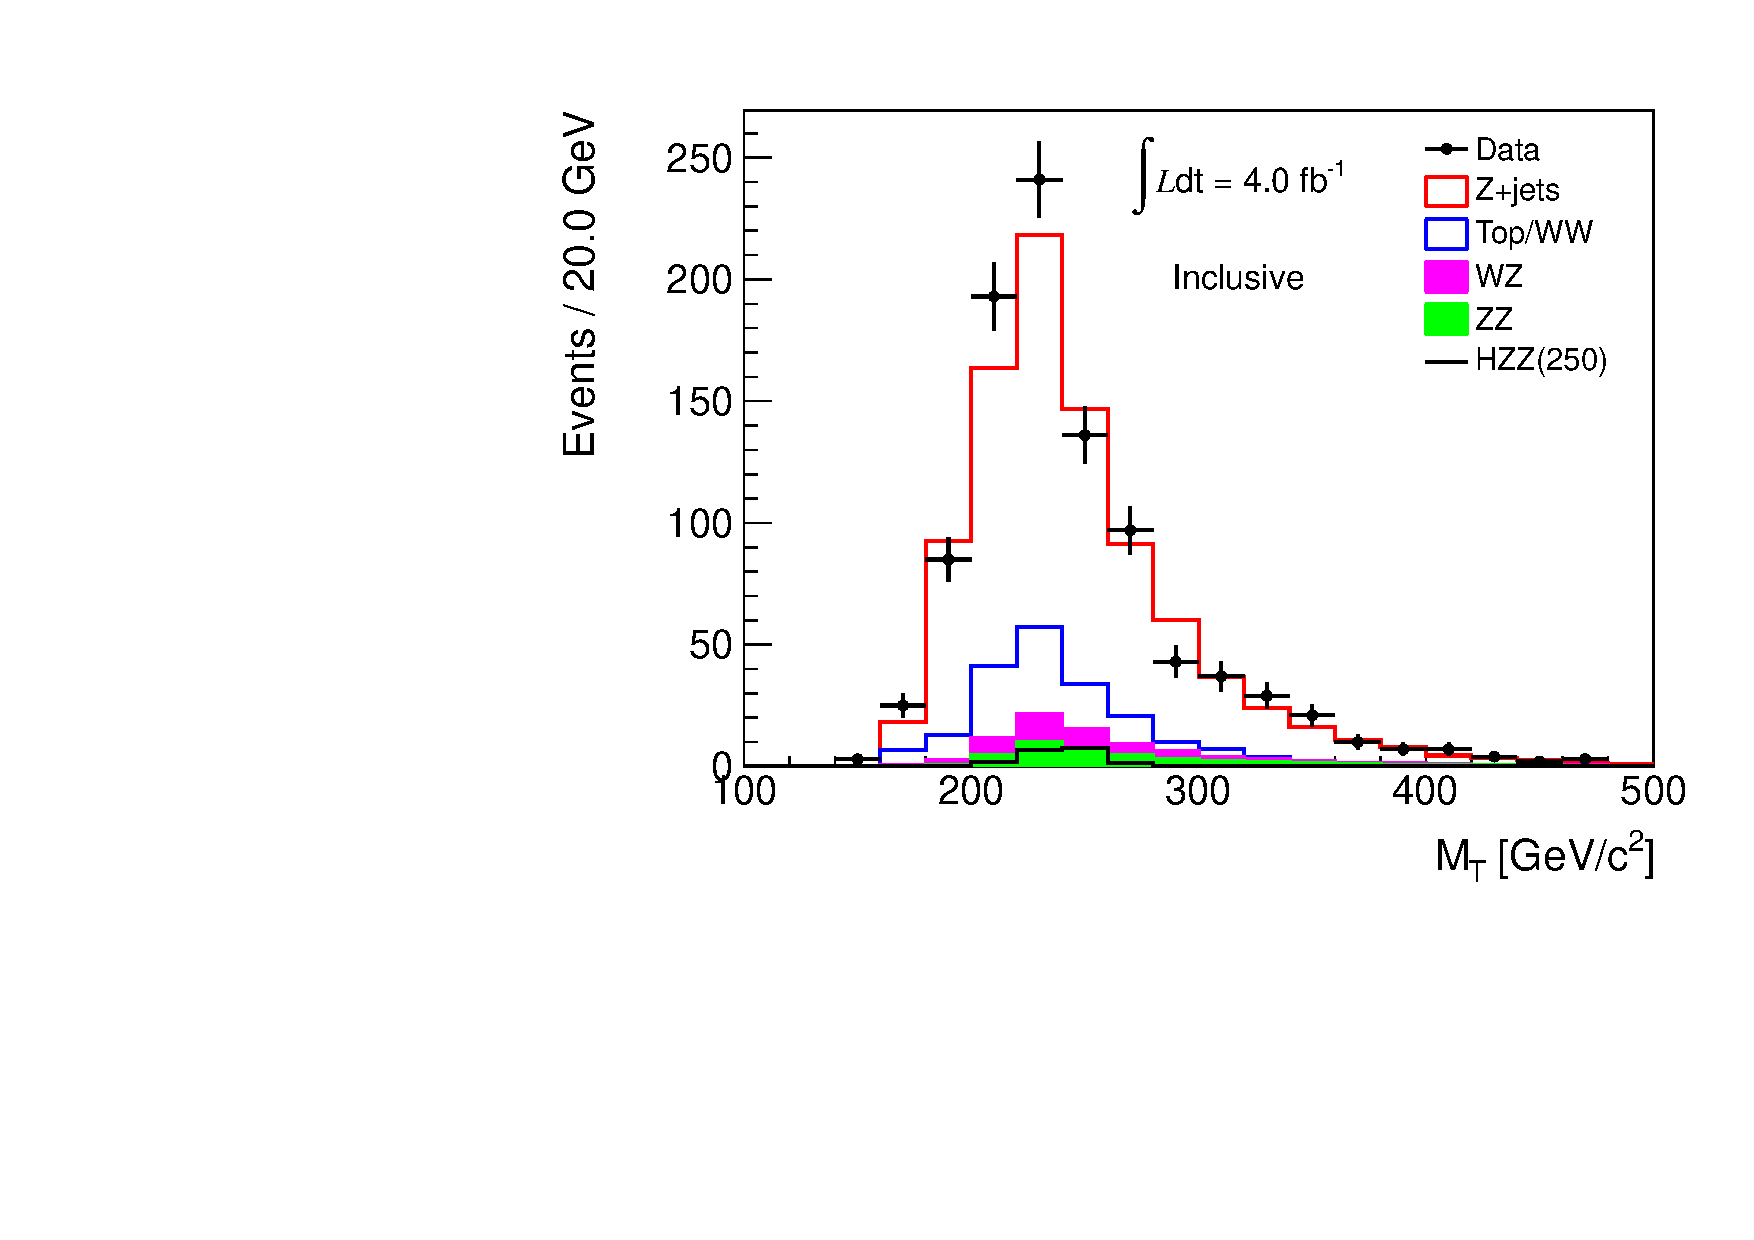
\includegraphics[width=.4\textwidth]{figures/presel_mH250_mm_mt_incl.pdf}}
\subfigure[0-Jet]{\label{subfig:mt_mm_0j}
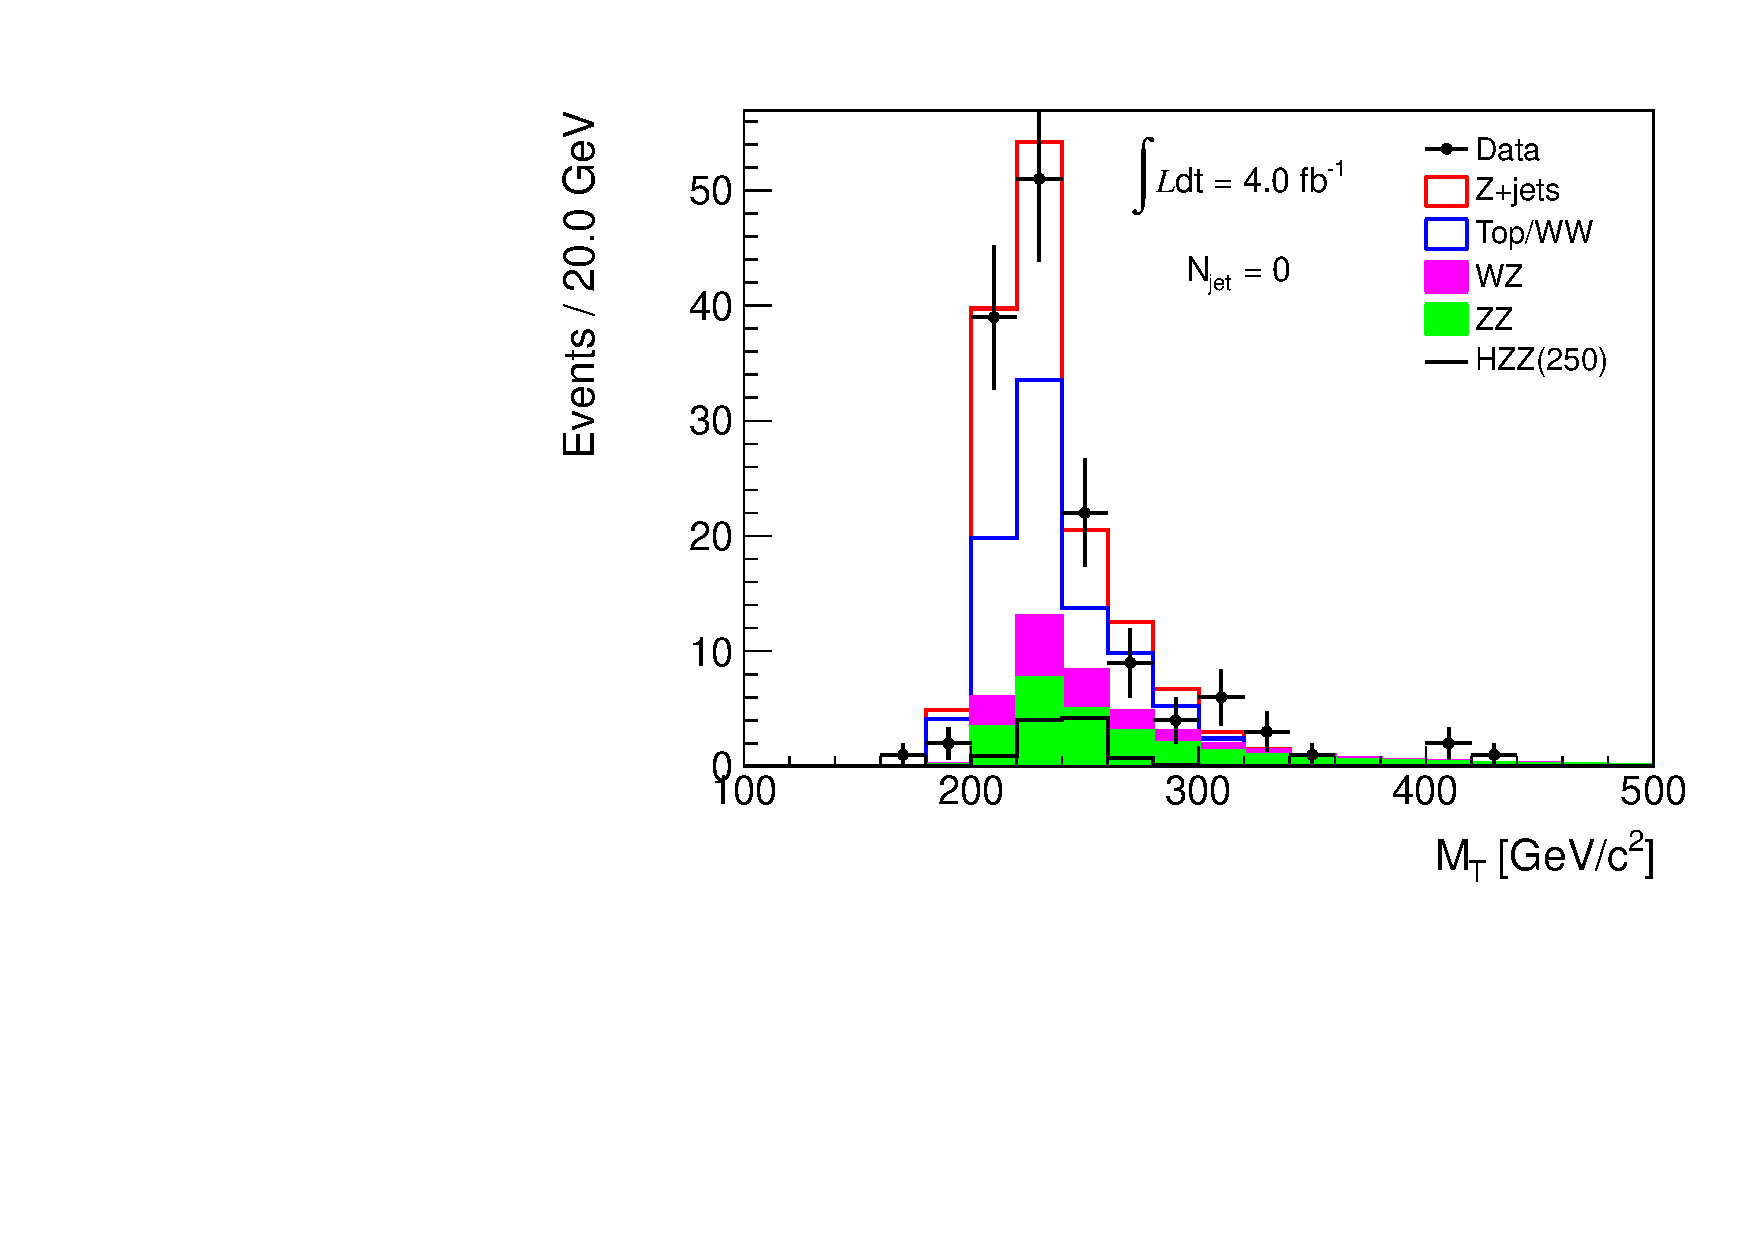
\includegraphics[width=.4\textwidth]{figures/presel_mH250_mm_mt_0j.pdf}} \\
\subfigure[1-Jet]{\label{subfig:mt_mm_1j}
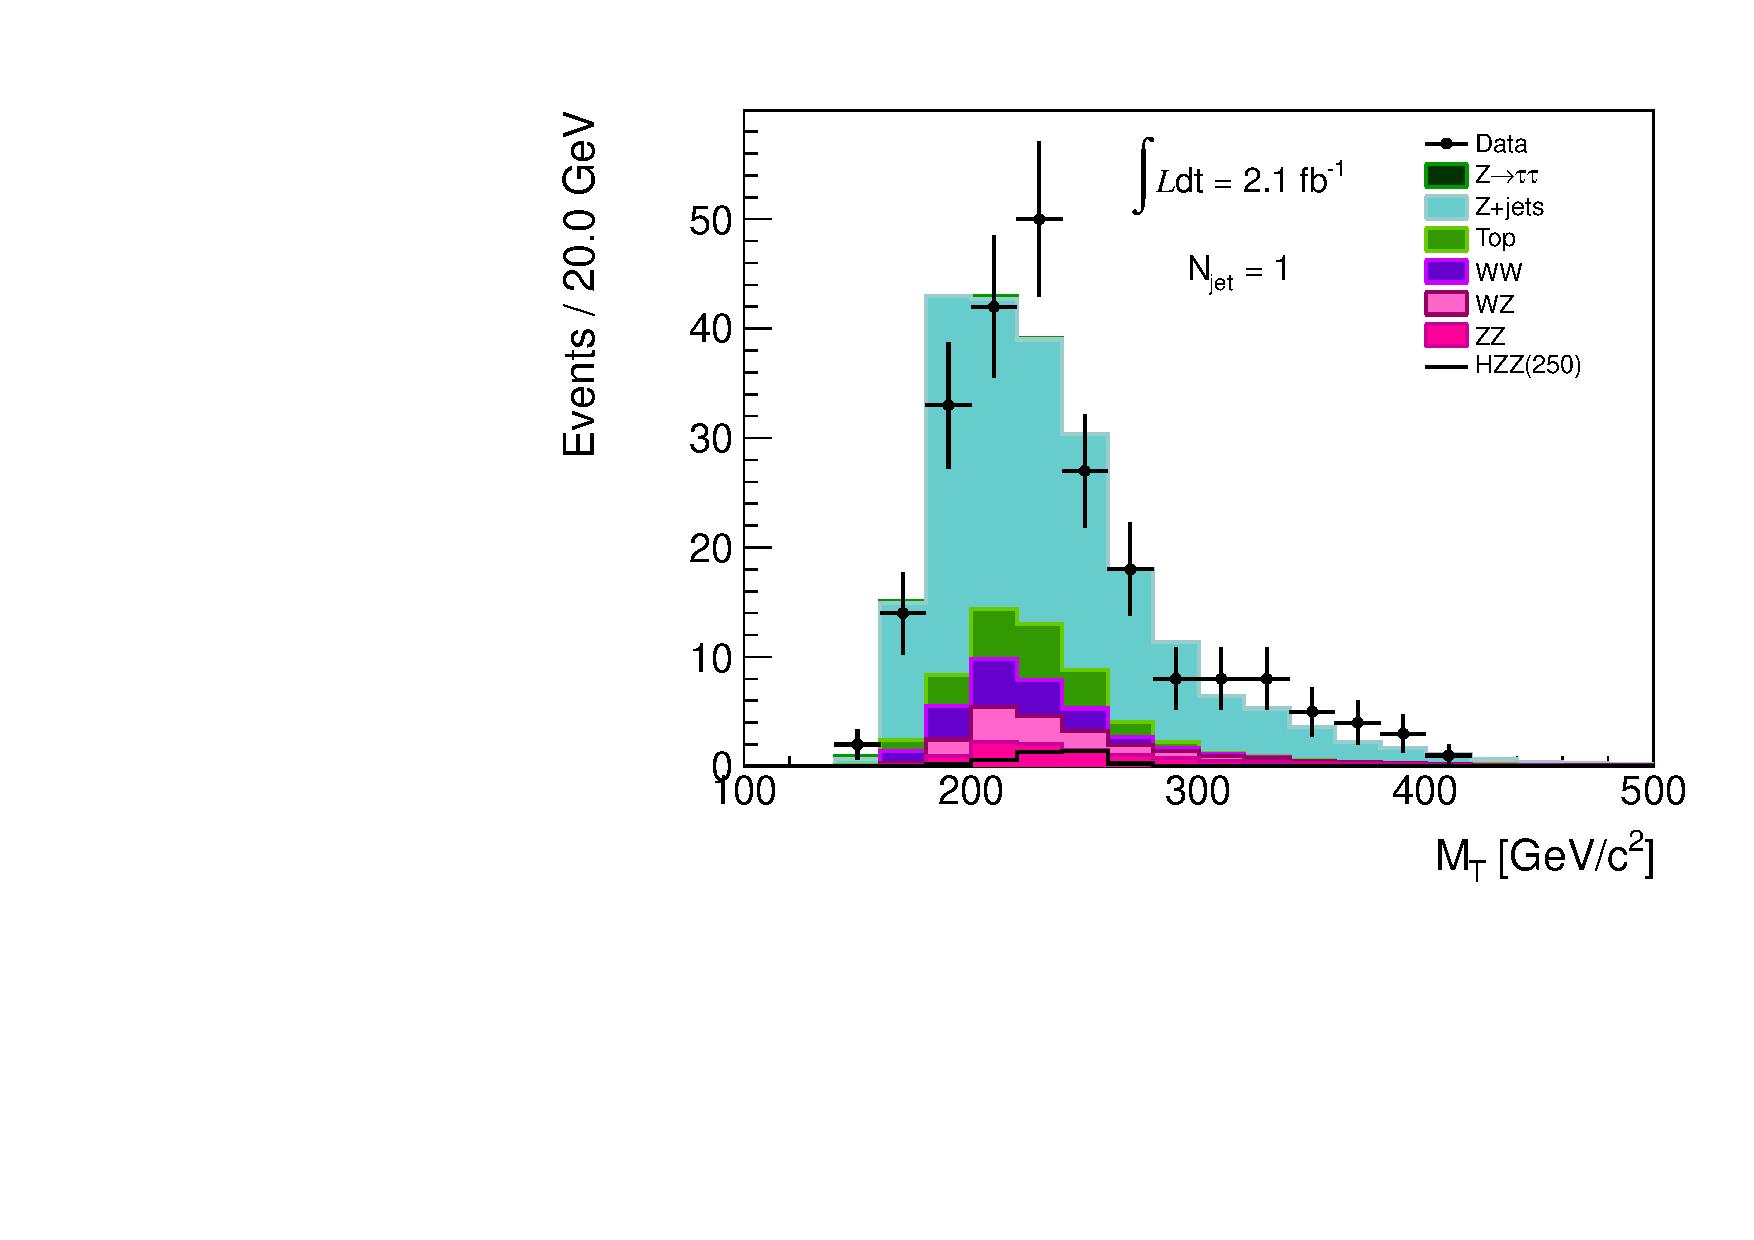
\includegraphics[width=.4\textwidth]{figures/presel_mH250_mm_mt_1j.pdf}}
\subfigure[$\geq$2 Jets]{\label{subfig:mt_mm_2j}
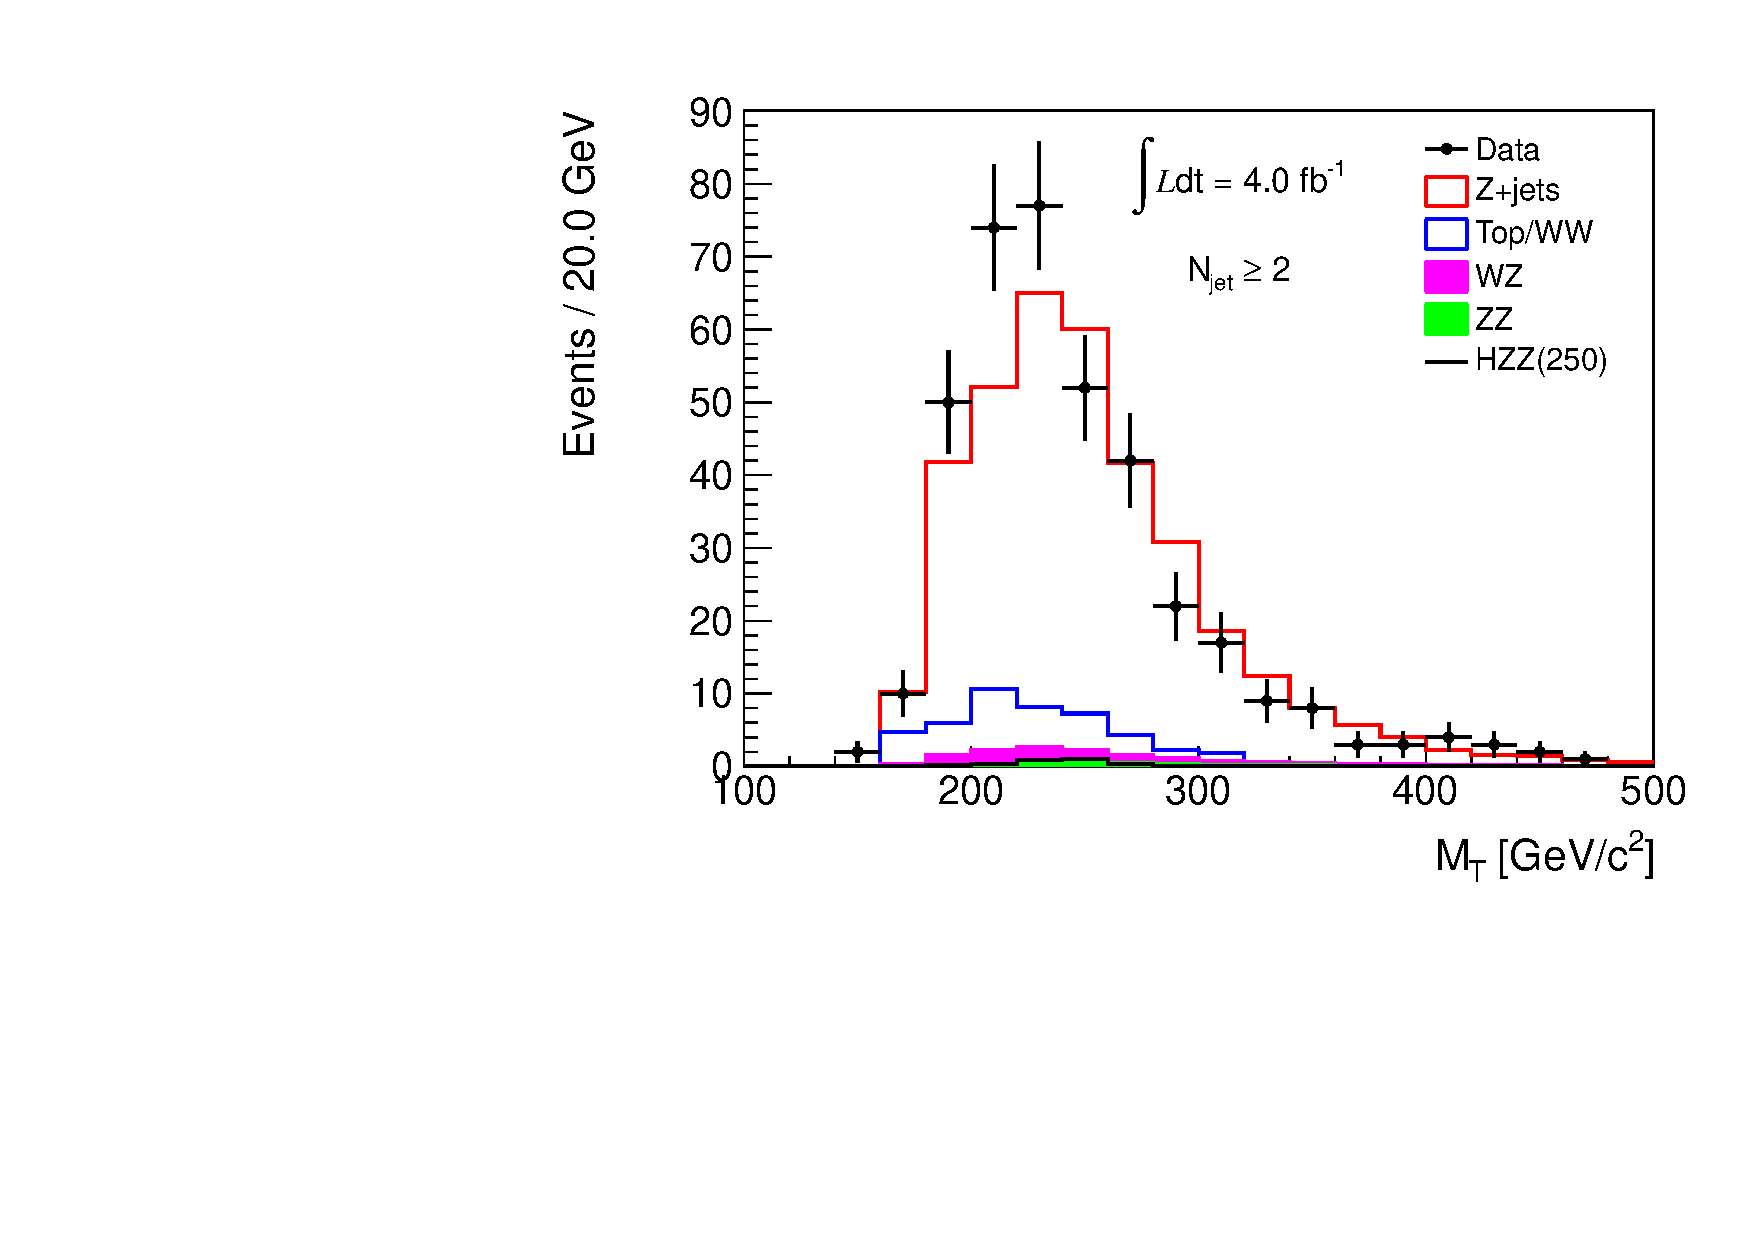
\includegraphics[width=.4\textwidth]{figures/presel_mH250_mm_mt_2j.pdf}}
\caption{Transverse mass distribution in the muon channel after the $\ZZ$ preselection observed in data corresponding to $2.1$~\ifb data in 
the Inclusive~\subref{subfig:mt_mm_incl}, 0-Jet~\subref{subfig:mt_mm_0j}, 1-Jet~\subref{subfig:mt_mm_1j} and 2-Jet~\subref{subfig:mt_mm_2j} bins, 
compared to the expected from simulation for signal and background. The MC backgrounds are scaled as appropriate and the photon+jets estimate of the 
Z+jets background is added to the stack.}
\label{fig:mt_zzpresel_mm}
\end{center}
\end{figure}
%%%%%%%%

%%%%%%%%
\begin{figure}[!hbtp]
\begin{center}
\subfigure[Inclusive]{\label{subfig:mt_ee_incl}
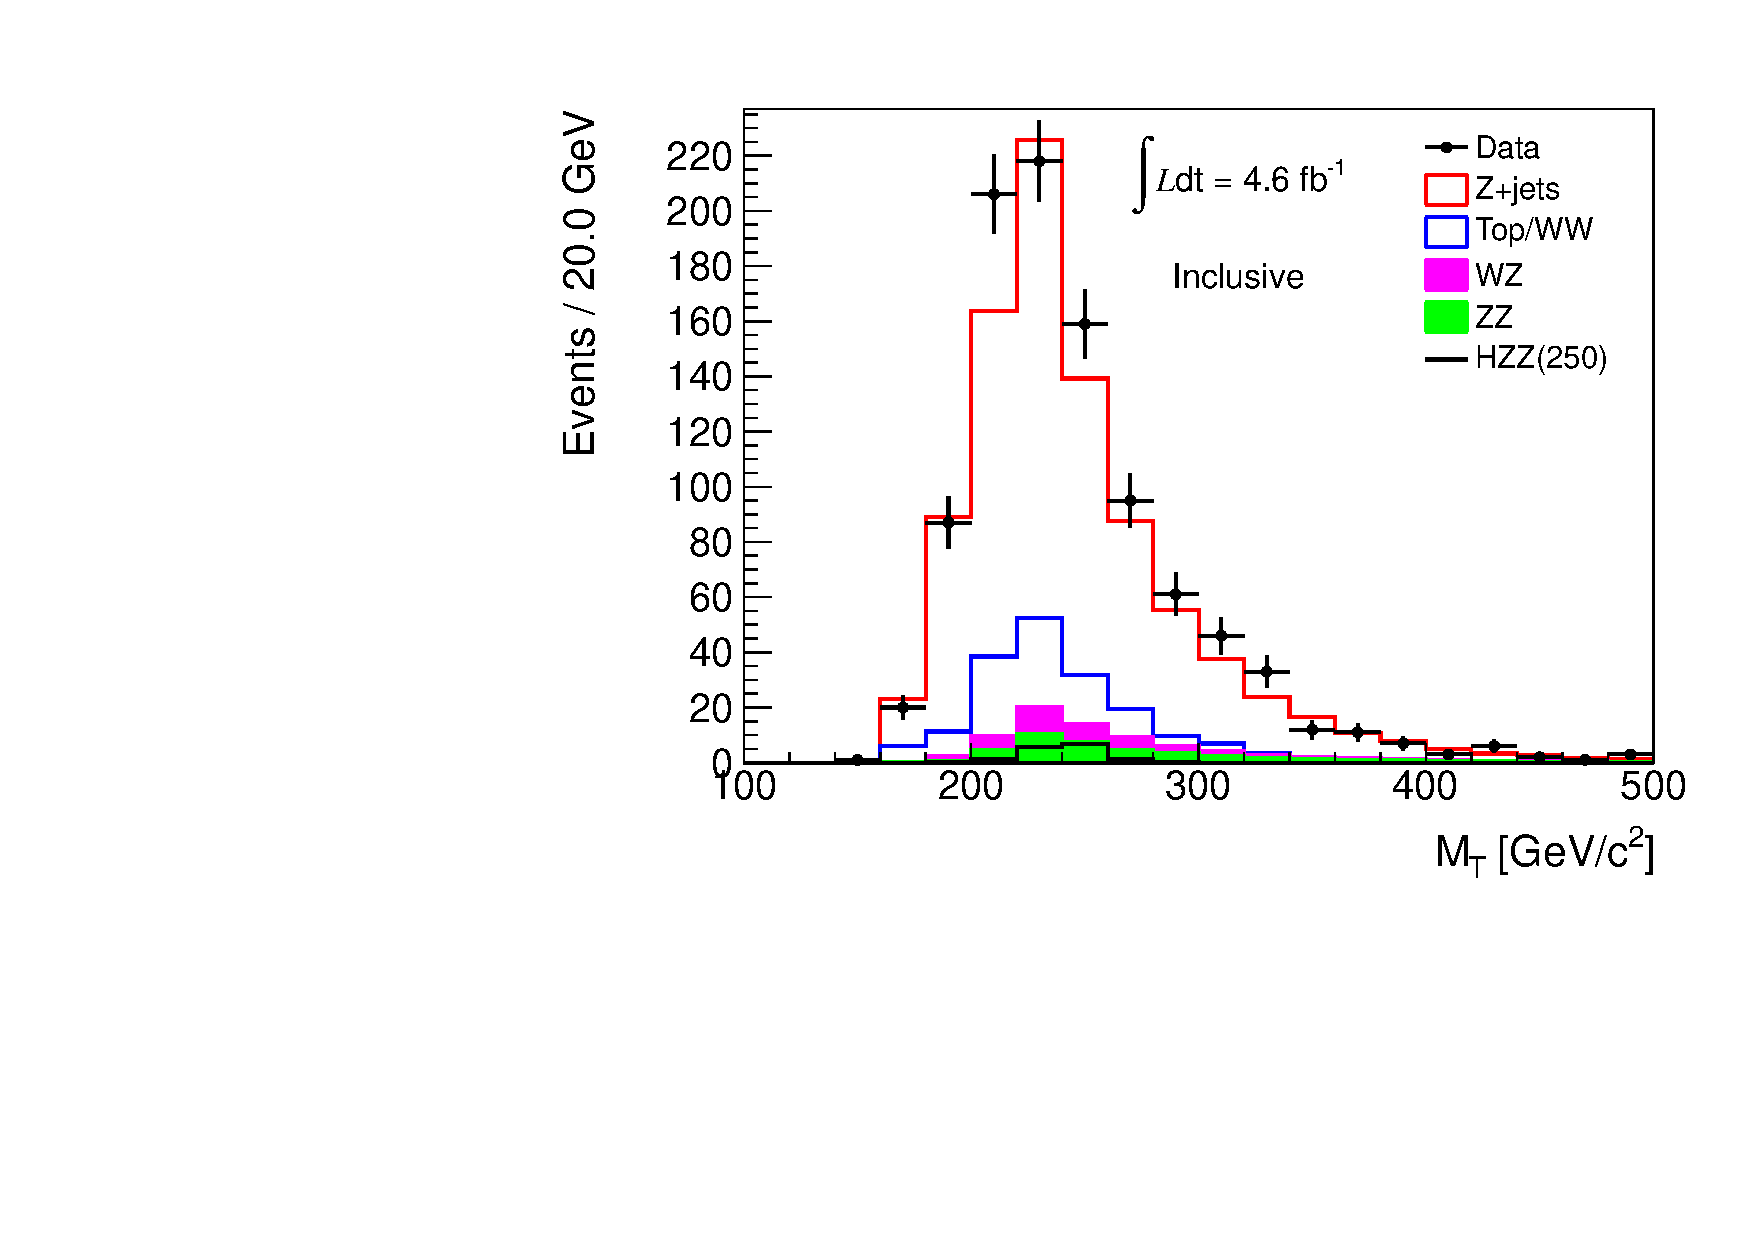
\includegraphics[width=.4\textwidth]{figures/presel_mH250_ee_mt_incl.pdf}}
\subfigure[0-Jet]{\label{subfig:mt_ee_0j}
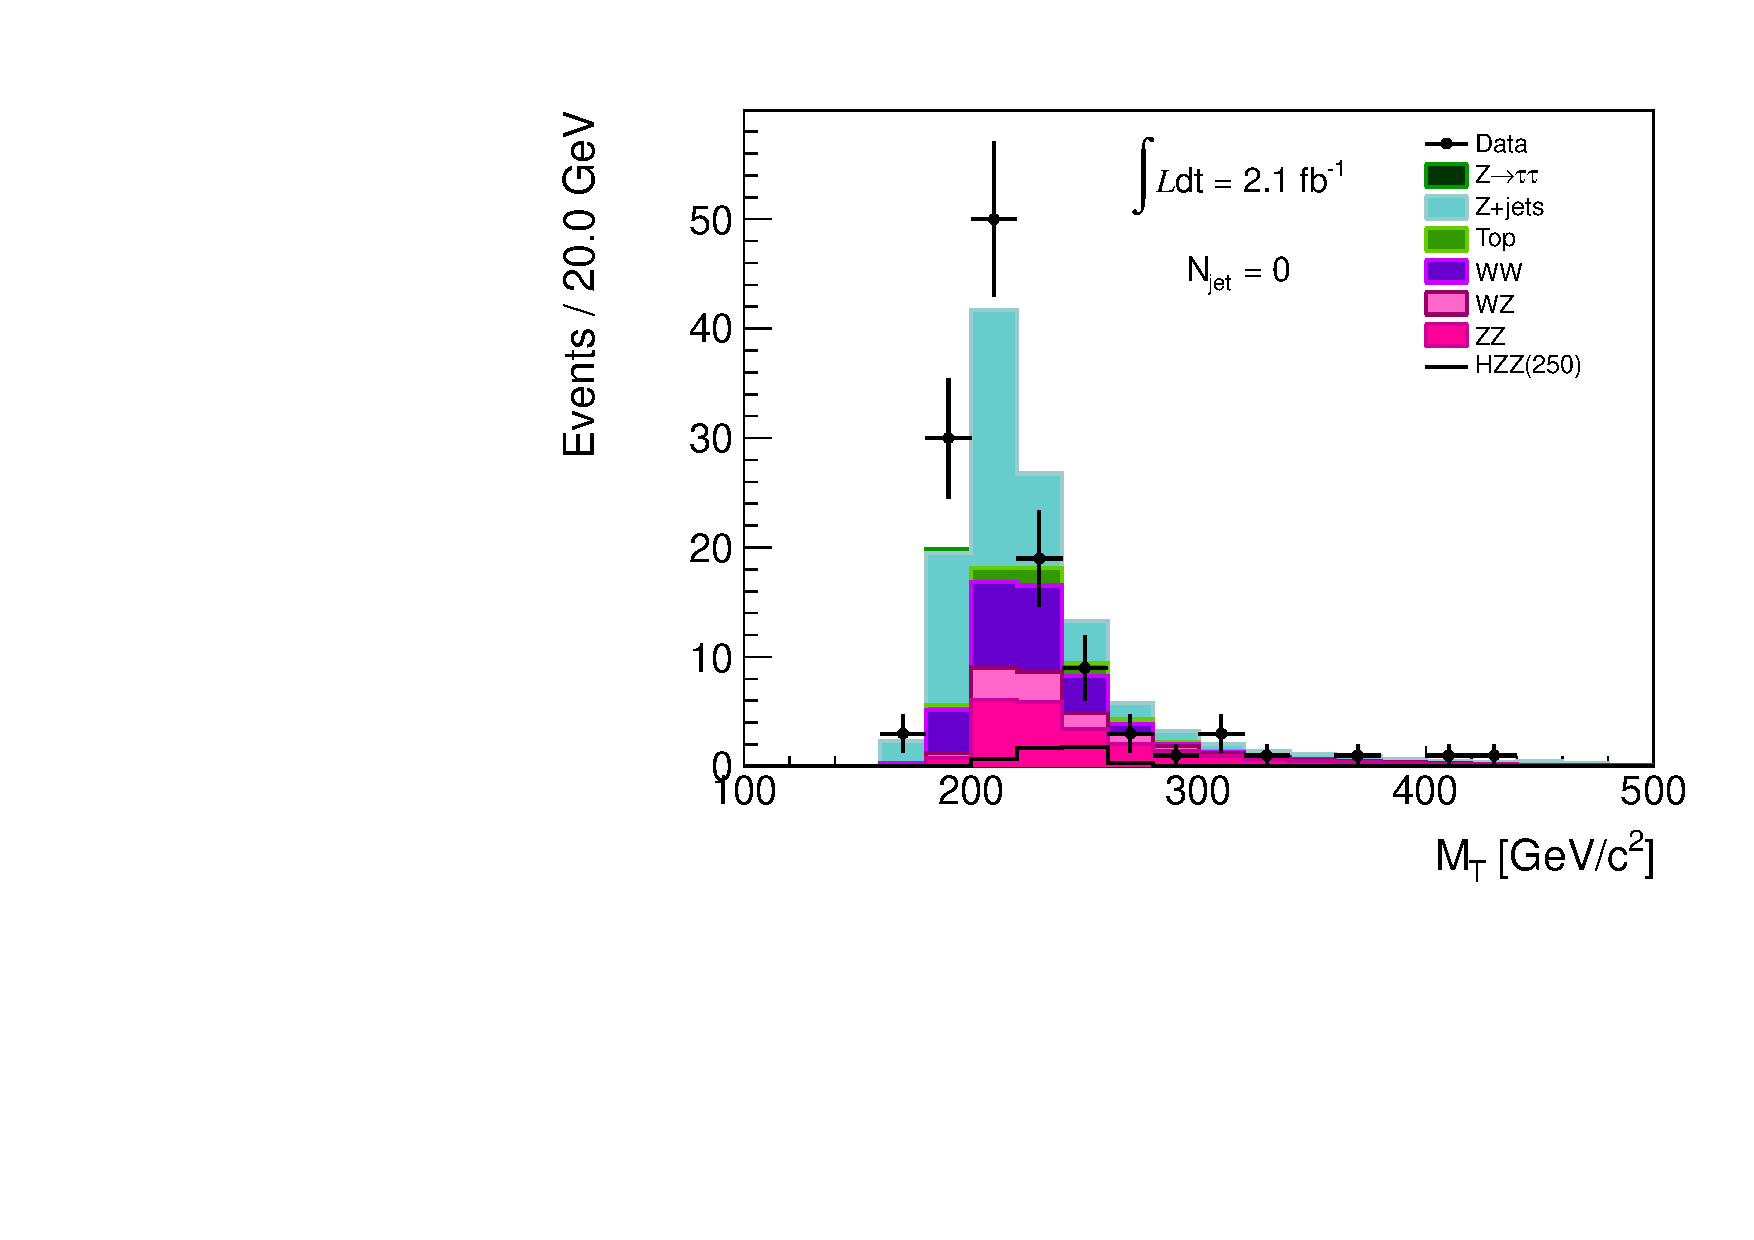
\includegraphics[width=.4\textwidth]{figures/presel_mH250_ee_mt_0j.pdf}} \\
\subfigure[1-Jet]{\label{subfig:mt_ee_1j}
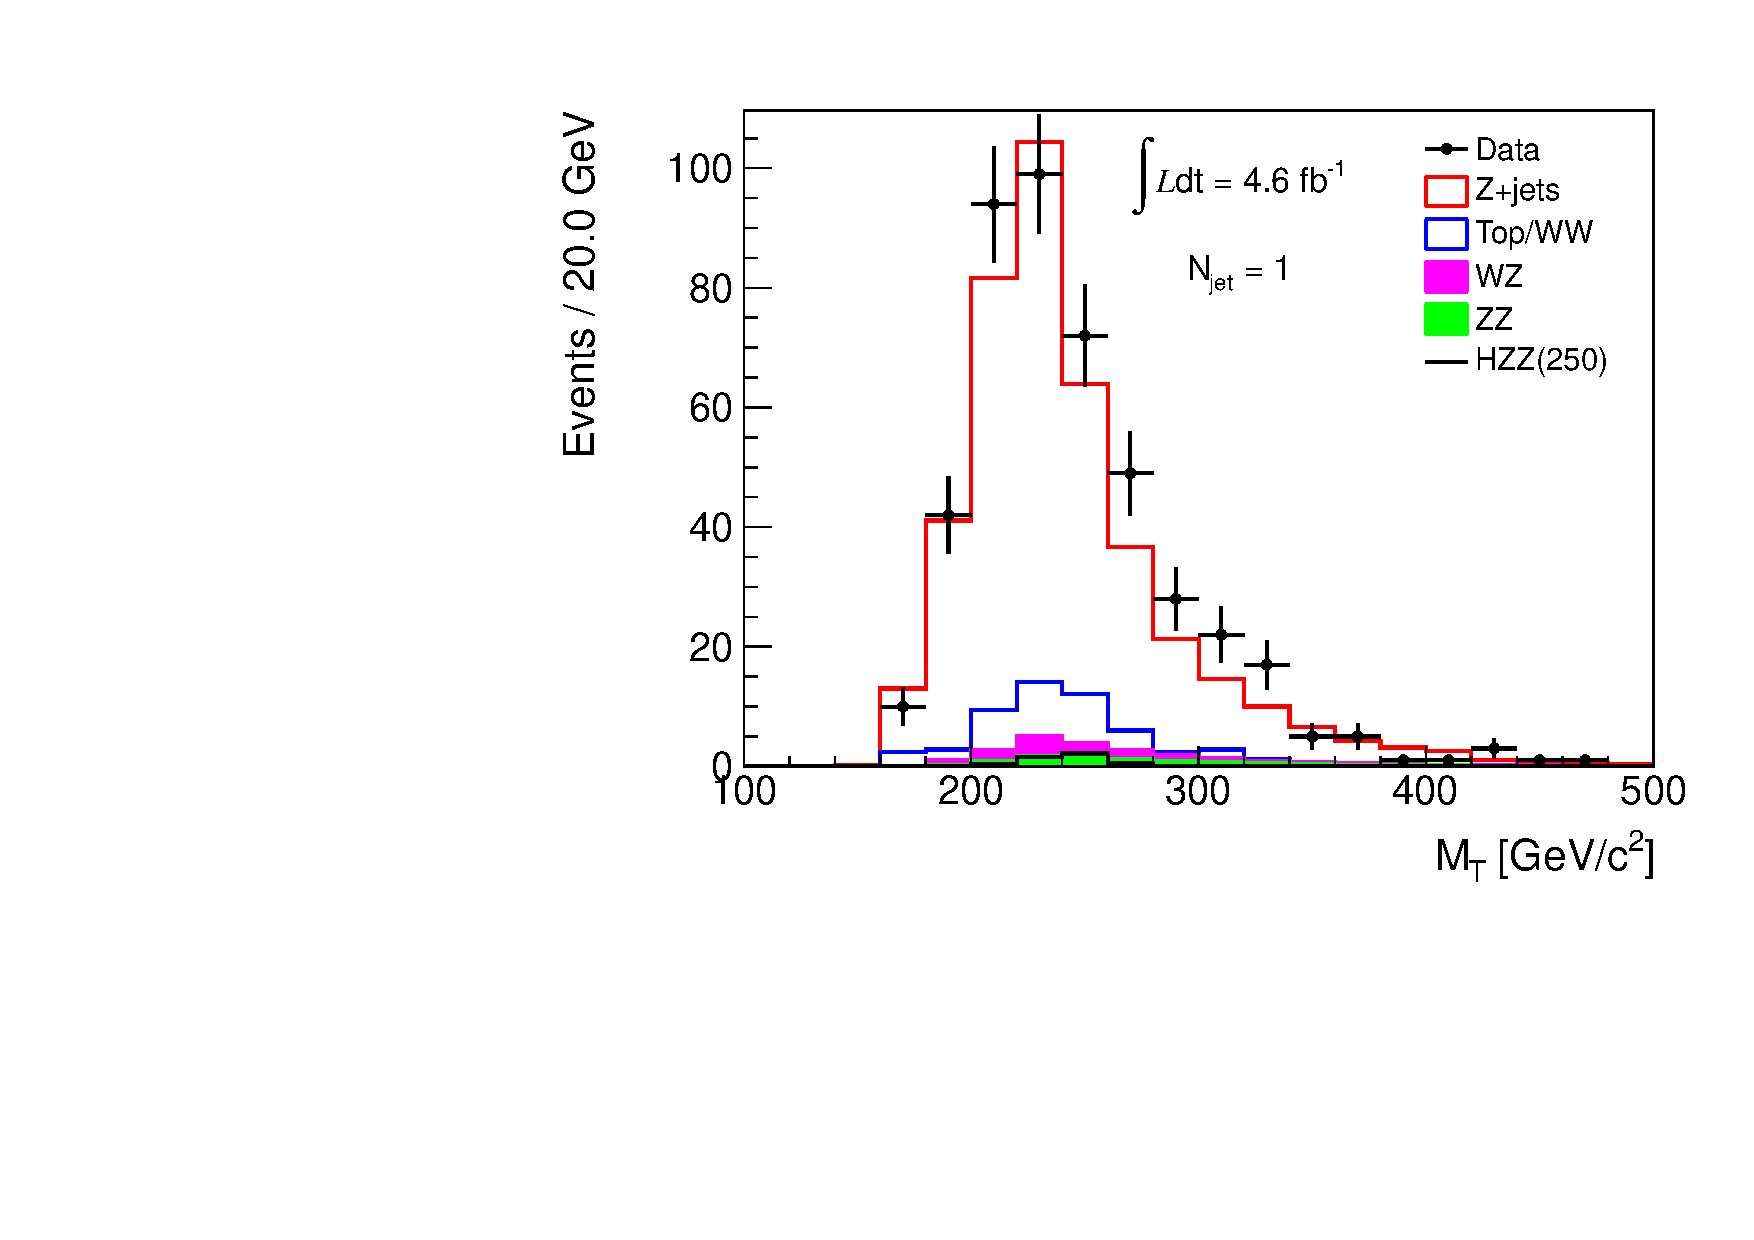
\includegraphics[width=.4\textwidth]{figures/presel_mH250_ee_mt_1j.pdf}}
\subfigure[$\geq$2 Jets]{\label{subfig:mt_ee_2j}
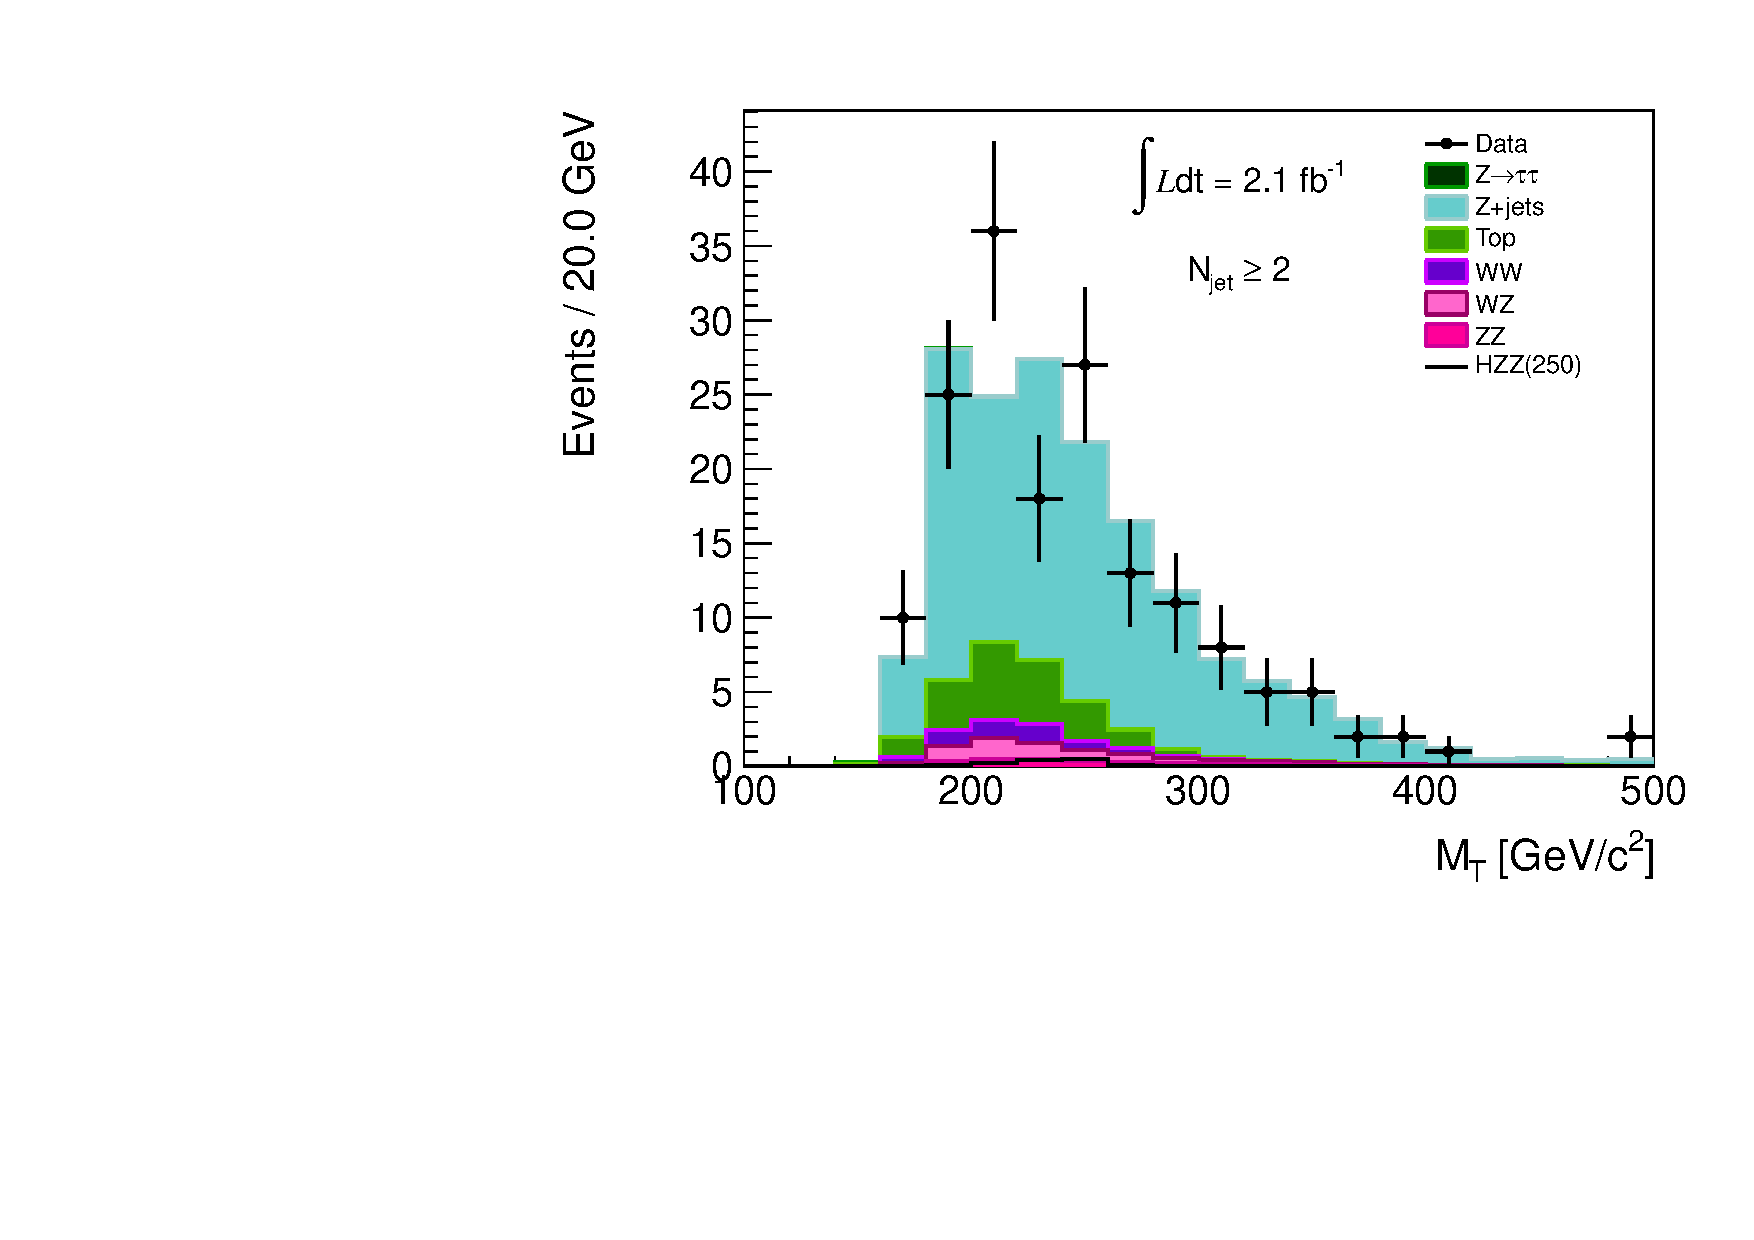
\includegraphics[width=.4\textwidth]{figures/presel_mH250_ee_mt_2j.pdf}}
\caption{Transverse mass distribution in the electron channel after the $\ZZ$ preselection observed in data corresponding to $2.1$~\ifb data in 
the Inclusive~\subref{subfig:mt_ee_incl}, 0-Jet~\subref{subfig:mt_ee_0j}, 1-Jet~\subref{subfig:mt_ee_1j} and 2-Jet~\subref{subfig:mt_ee_2j} bins, 
compared to the expected from simulation for signal and background. The MC backgrounds are scaled as appropriate and the photon+jets estimate of the 
Z+jets background is added to the stack.}
\label{fig:mt_zzpresel_ee}
\end{center}
\end{figure}
%%%%%%%%

%%%%%%%%
\begin{figure}[!hbtp]
\begin{center}
\subfigure[Inclusive]{\label{subfig:dphijetmet_mm_incl}
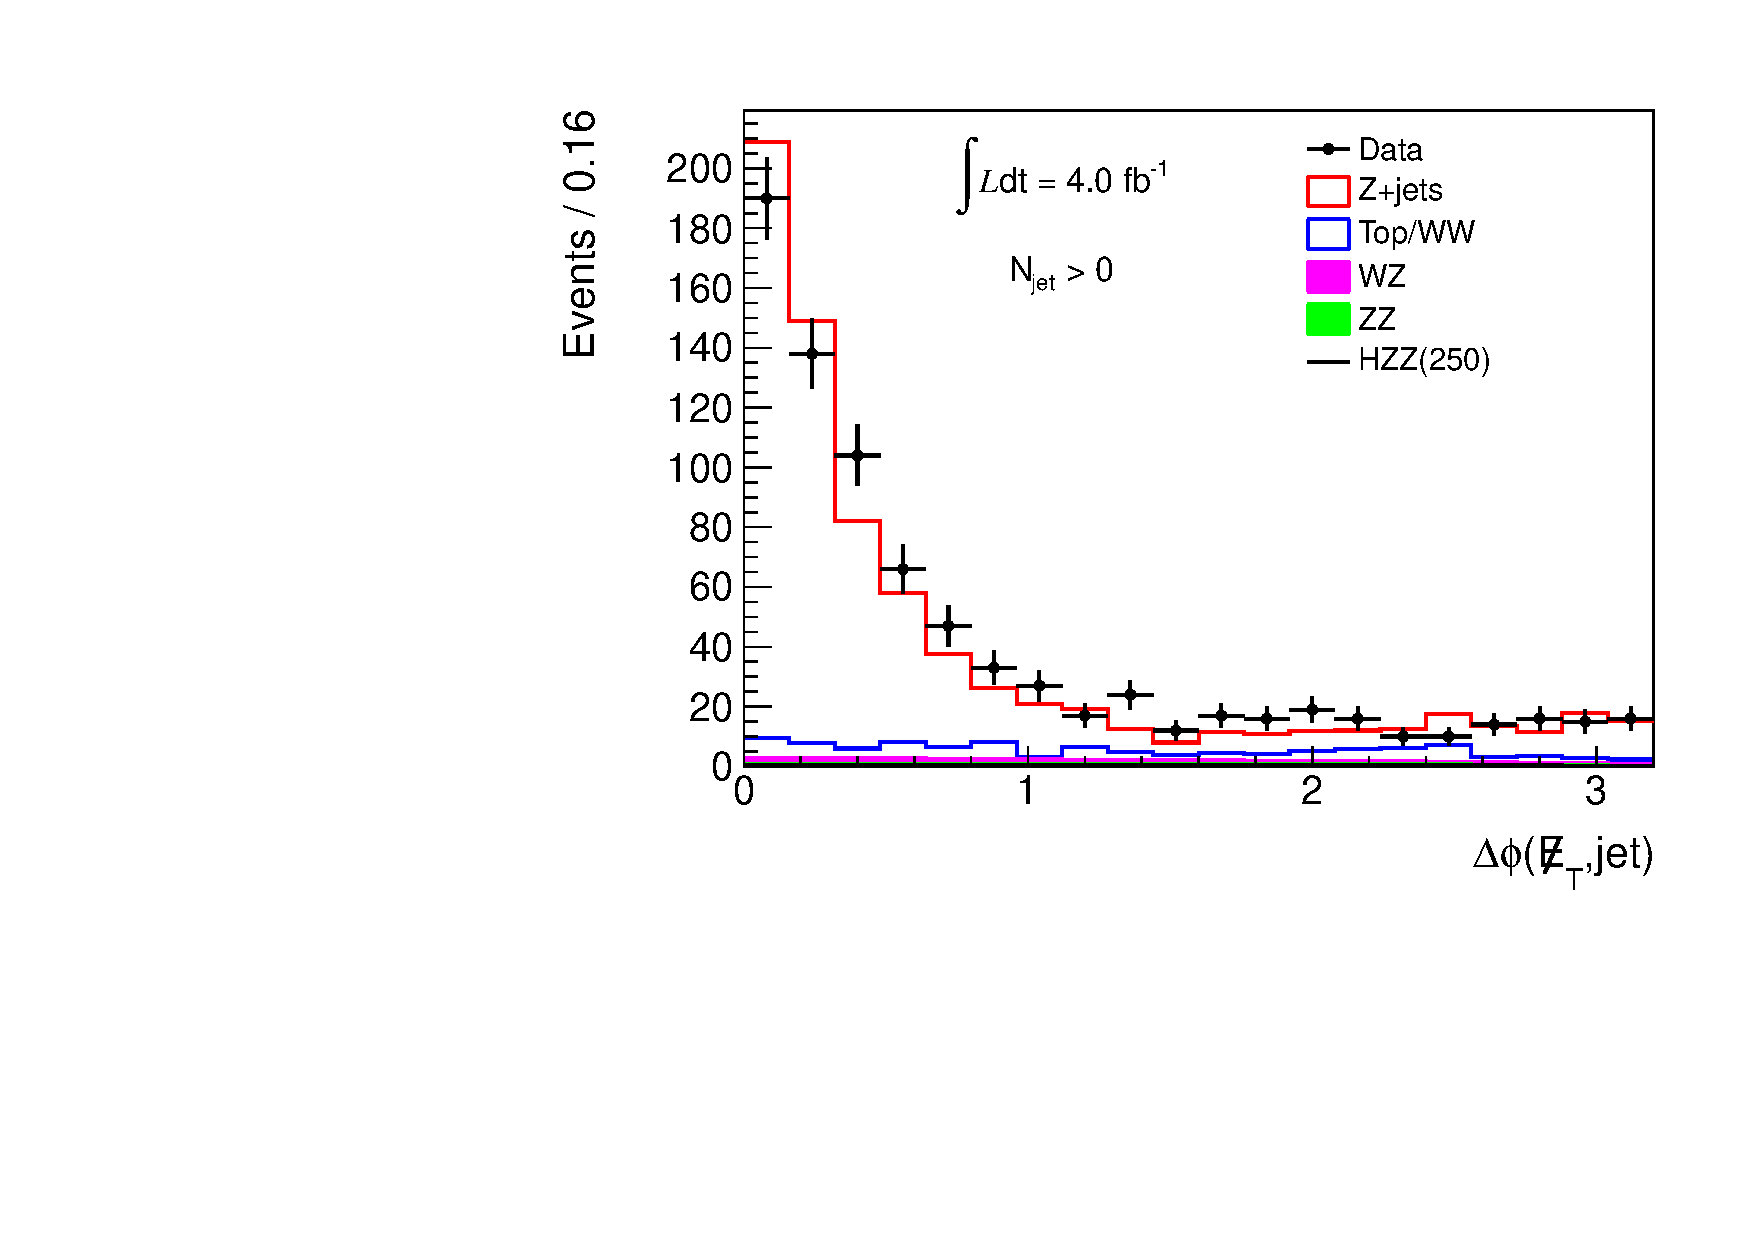
\includegraphics[width=.3\textwidth]{figures/presel_mH250_mm_dphijetmet_incl.pdf}}
\subfigure[1-Jet]{\label{subfig:dphijetmet_mm_1j}
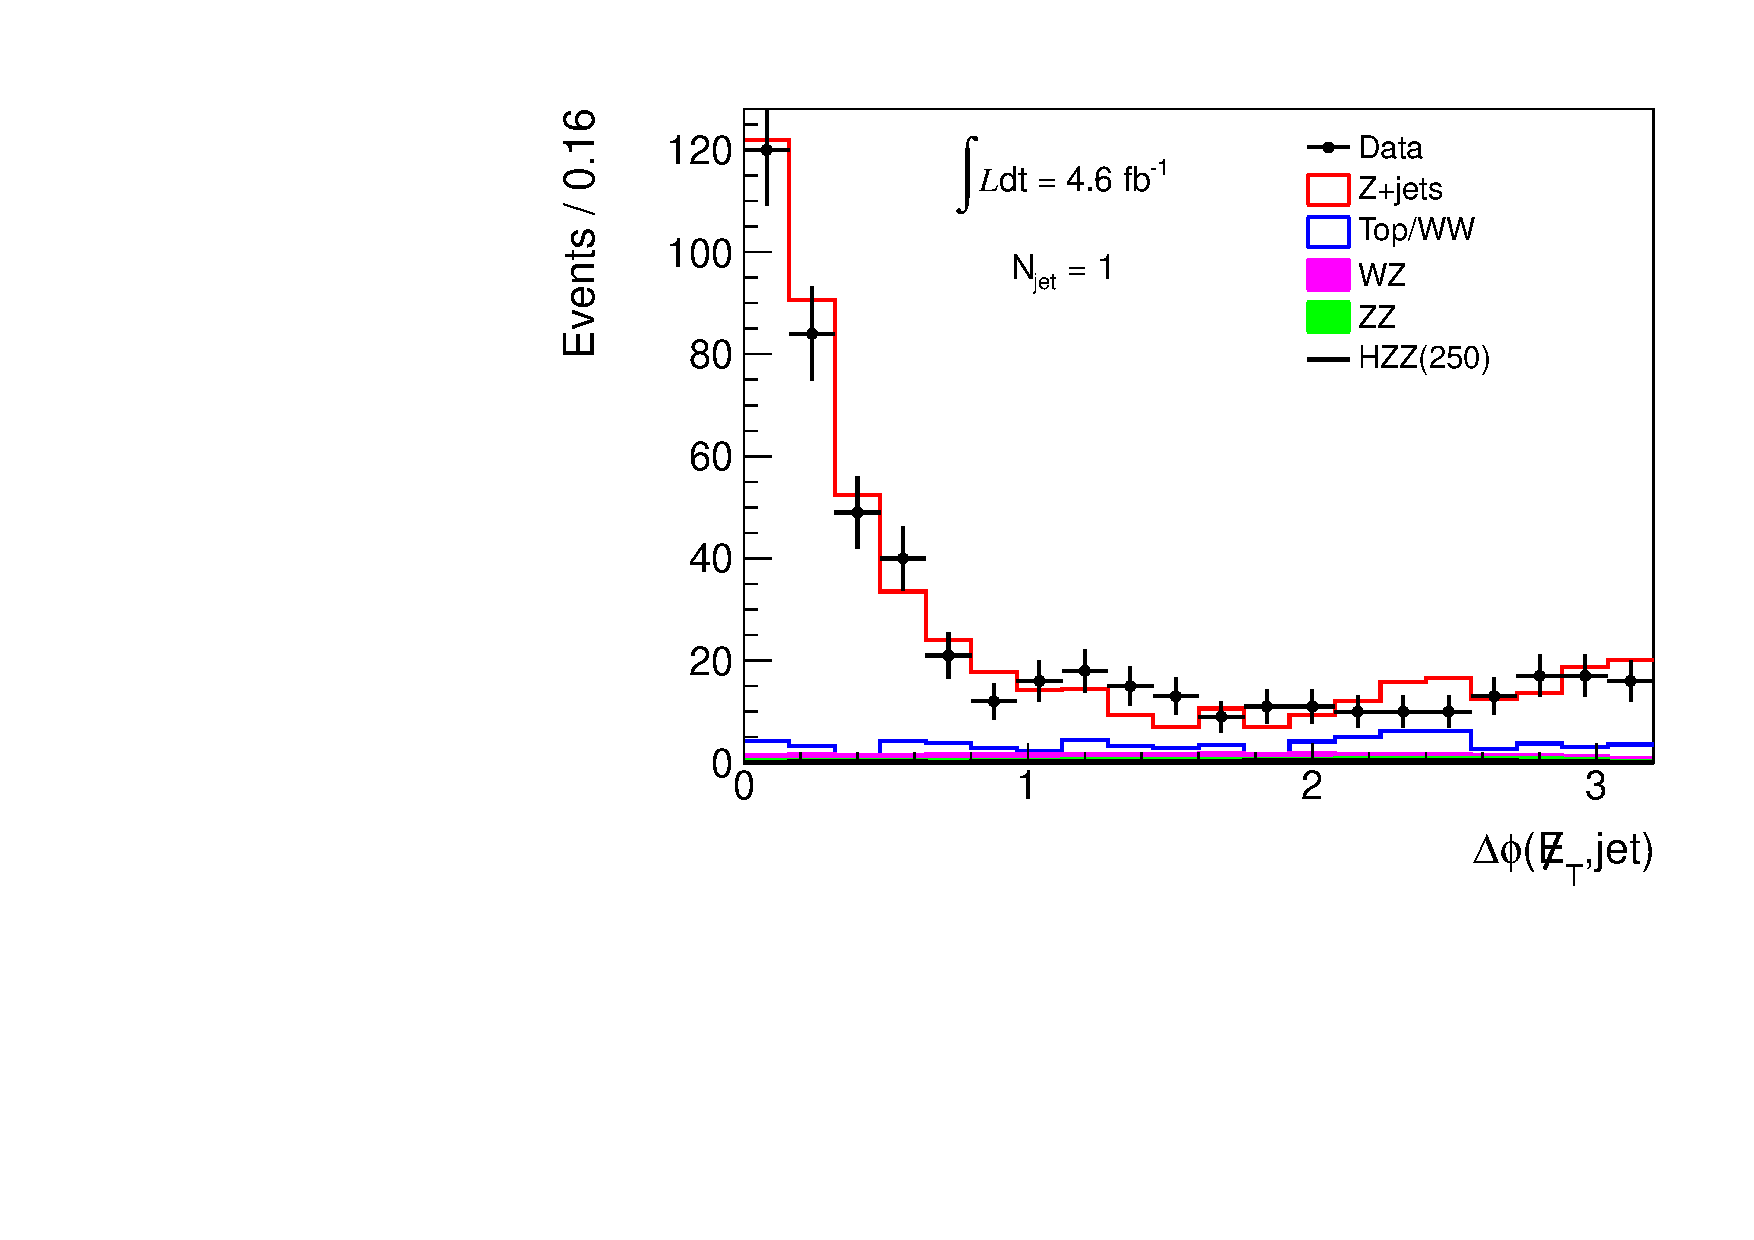
\includegraphics[width=.3\textwidth]{figures/presel_mH250_mm_dphijetmet_1j.pdf}}
\subfigure[$\geq$2 Jets]{\label{subfig:dphijetmet_mm_2j}
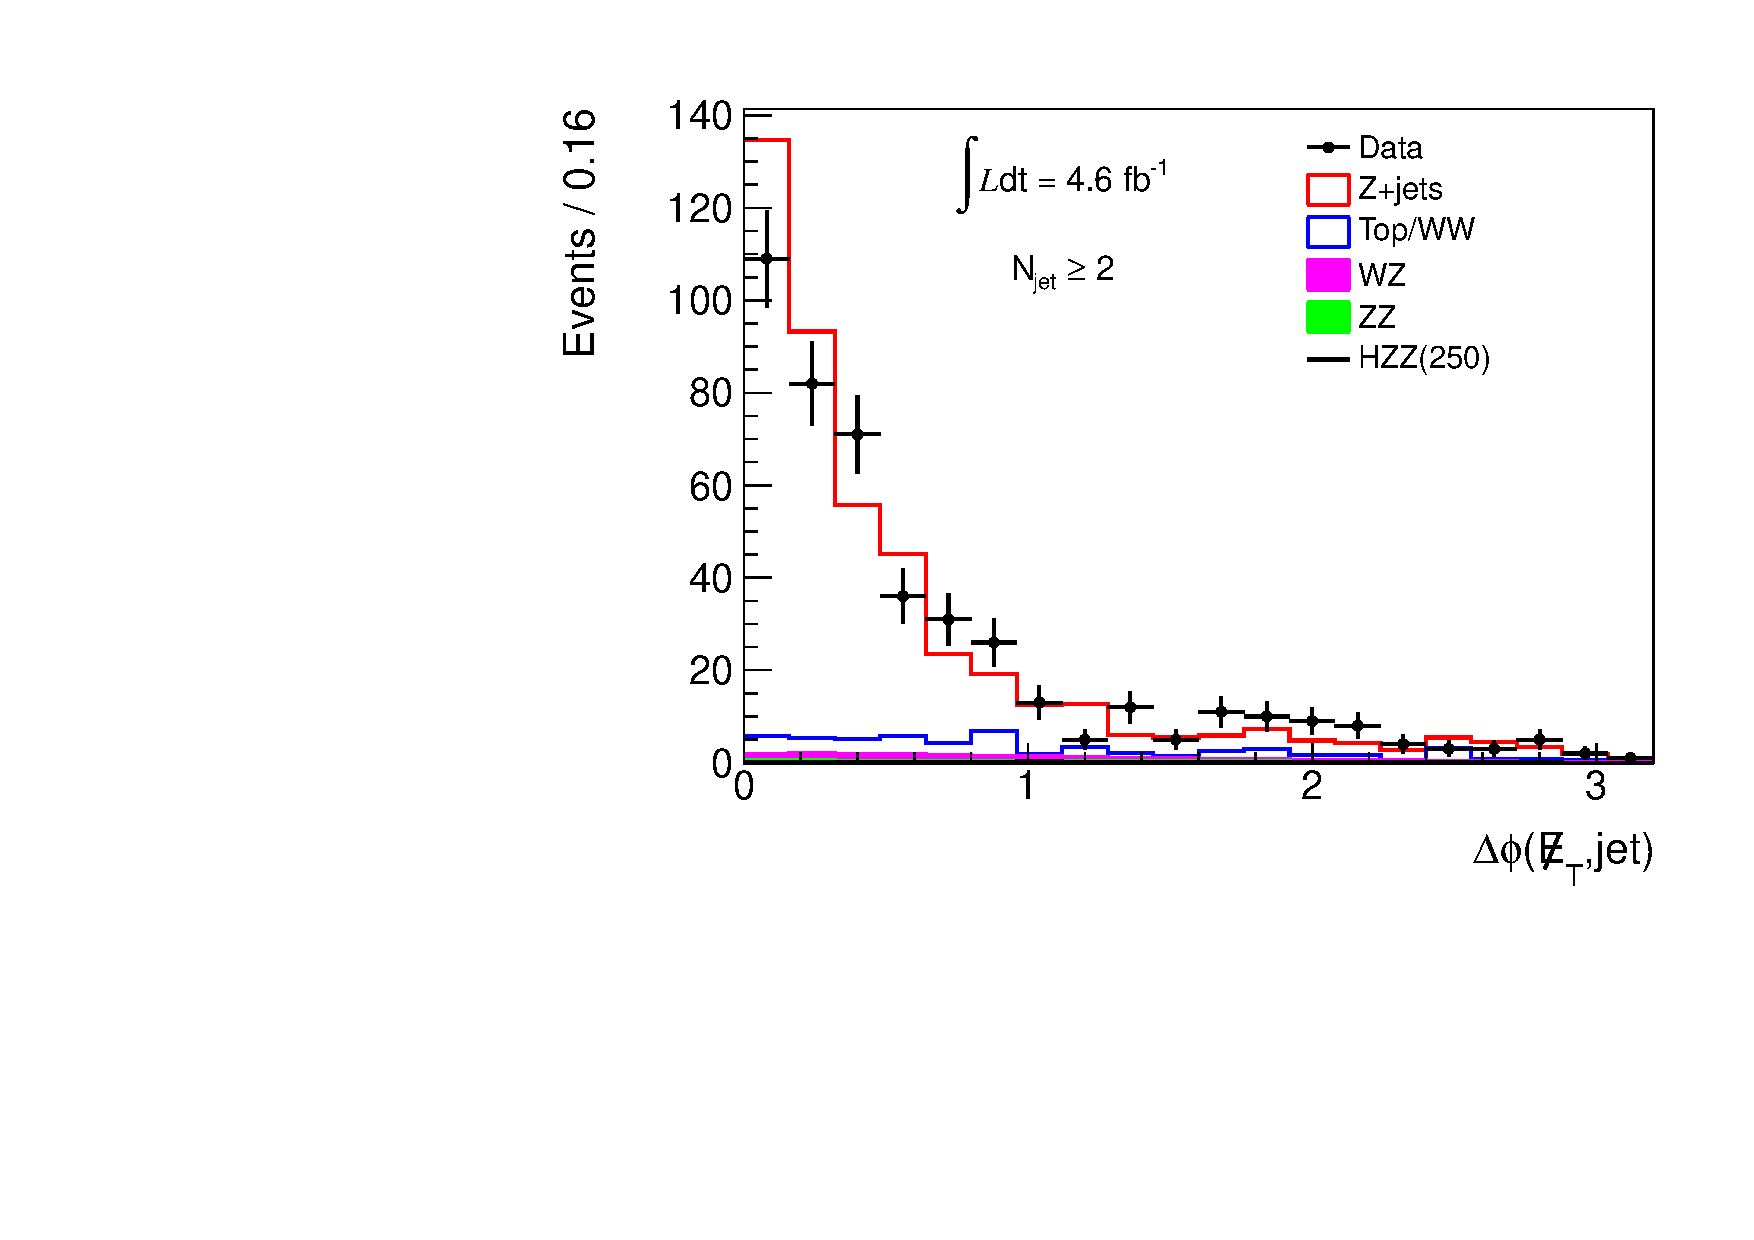
\includegraphics[width=.3\textwidth]{figures/presel_mH250_mm_dphijetmet_2j.pdf}}
\caption{Azimuthal angle separation between \met and the closest jet in the muon channel after the $\ZZ$ preselection observed in data corresponding 
to $2.1$~\ifb data in the Inclusive~\subref{subfig:dphijetmet_mm_incl}, 1-Jet~\subref{subfig:dphijetmet_mm_1j} and 
2-Jet~\subref{subfig:dphijetmet_mm_2j} bins, compared to the expected from simulation for signal and background. The MC backgrounds are scaled as appropriate and 
the photon+jets estimate of the Z+jets background is added to the stack.}
\label{fig:dphijetmet_zzpresel_mm}
\end{center}
\end{figure}
%%%%%%%%

%%%%%%%%
\begin{figure}[!hbtp]
\begin{center}
\subfigure[Inclusive]{\label{subfig:dphijetmet_ee_incl}
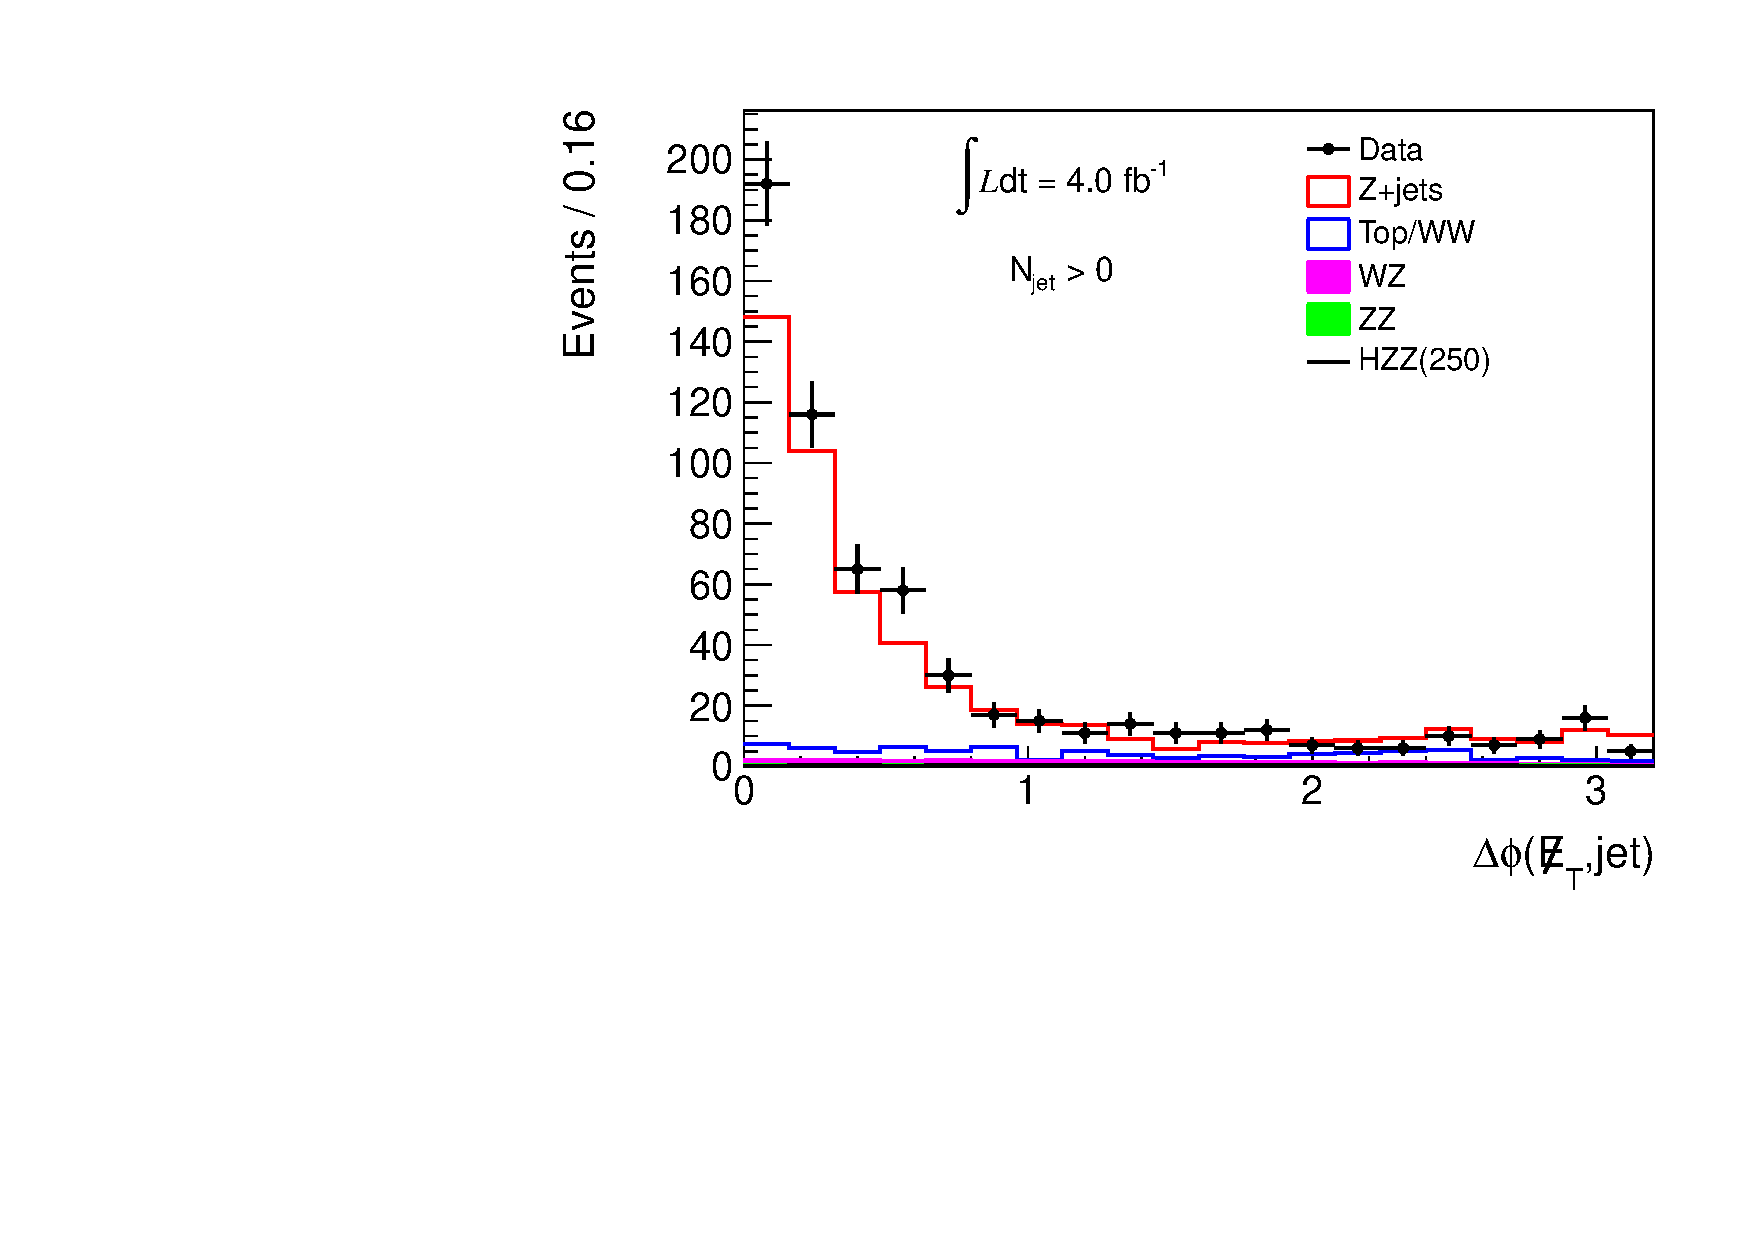
\includegraphics[width=.3\textwidth]{figures/presel_mH250_ee_dphijetmet_incl.pdf}}
\subfigure[1-Jet]{\label{subfig:dphijetmet_ee_1j}
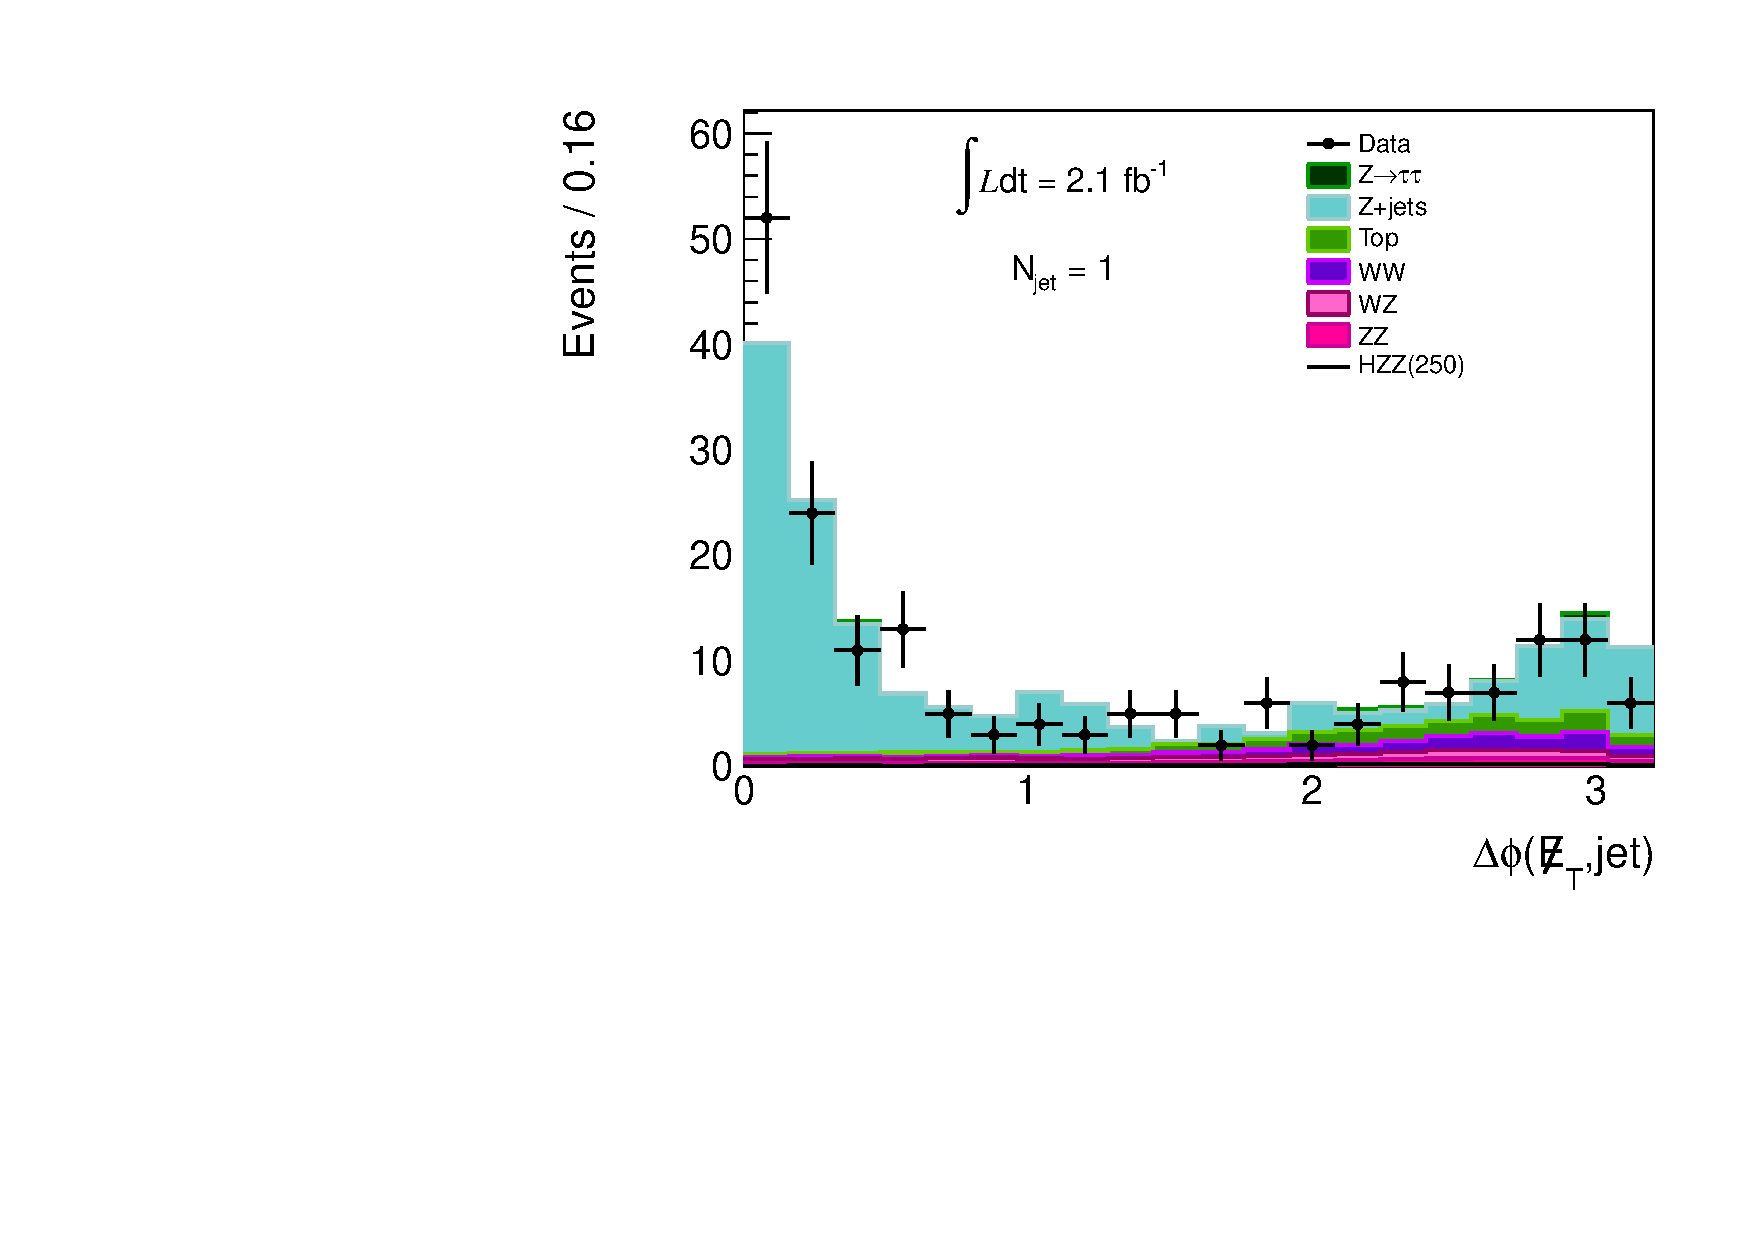
\includegraphics[width=.3\textwidth]{figures/presel_mH250_ee_dphijetmet_1j.pdf}}
\subfigure[$\geq$2 Jets]{\label{subfig:dphijetmet_ee_2j}
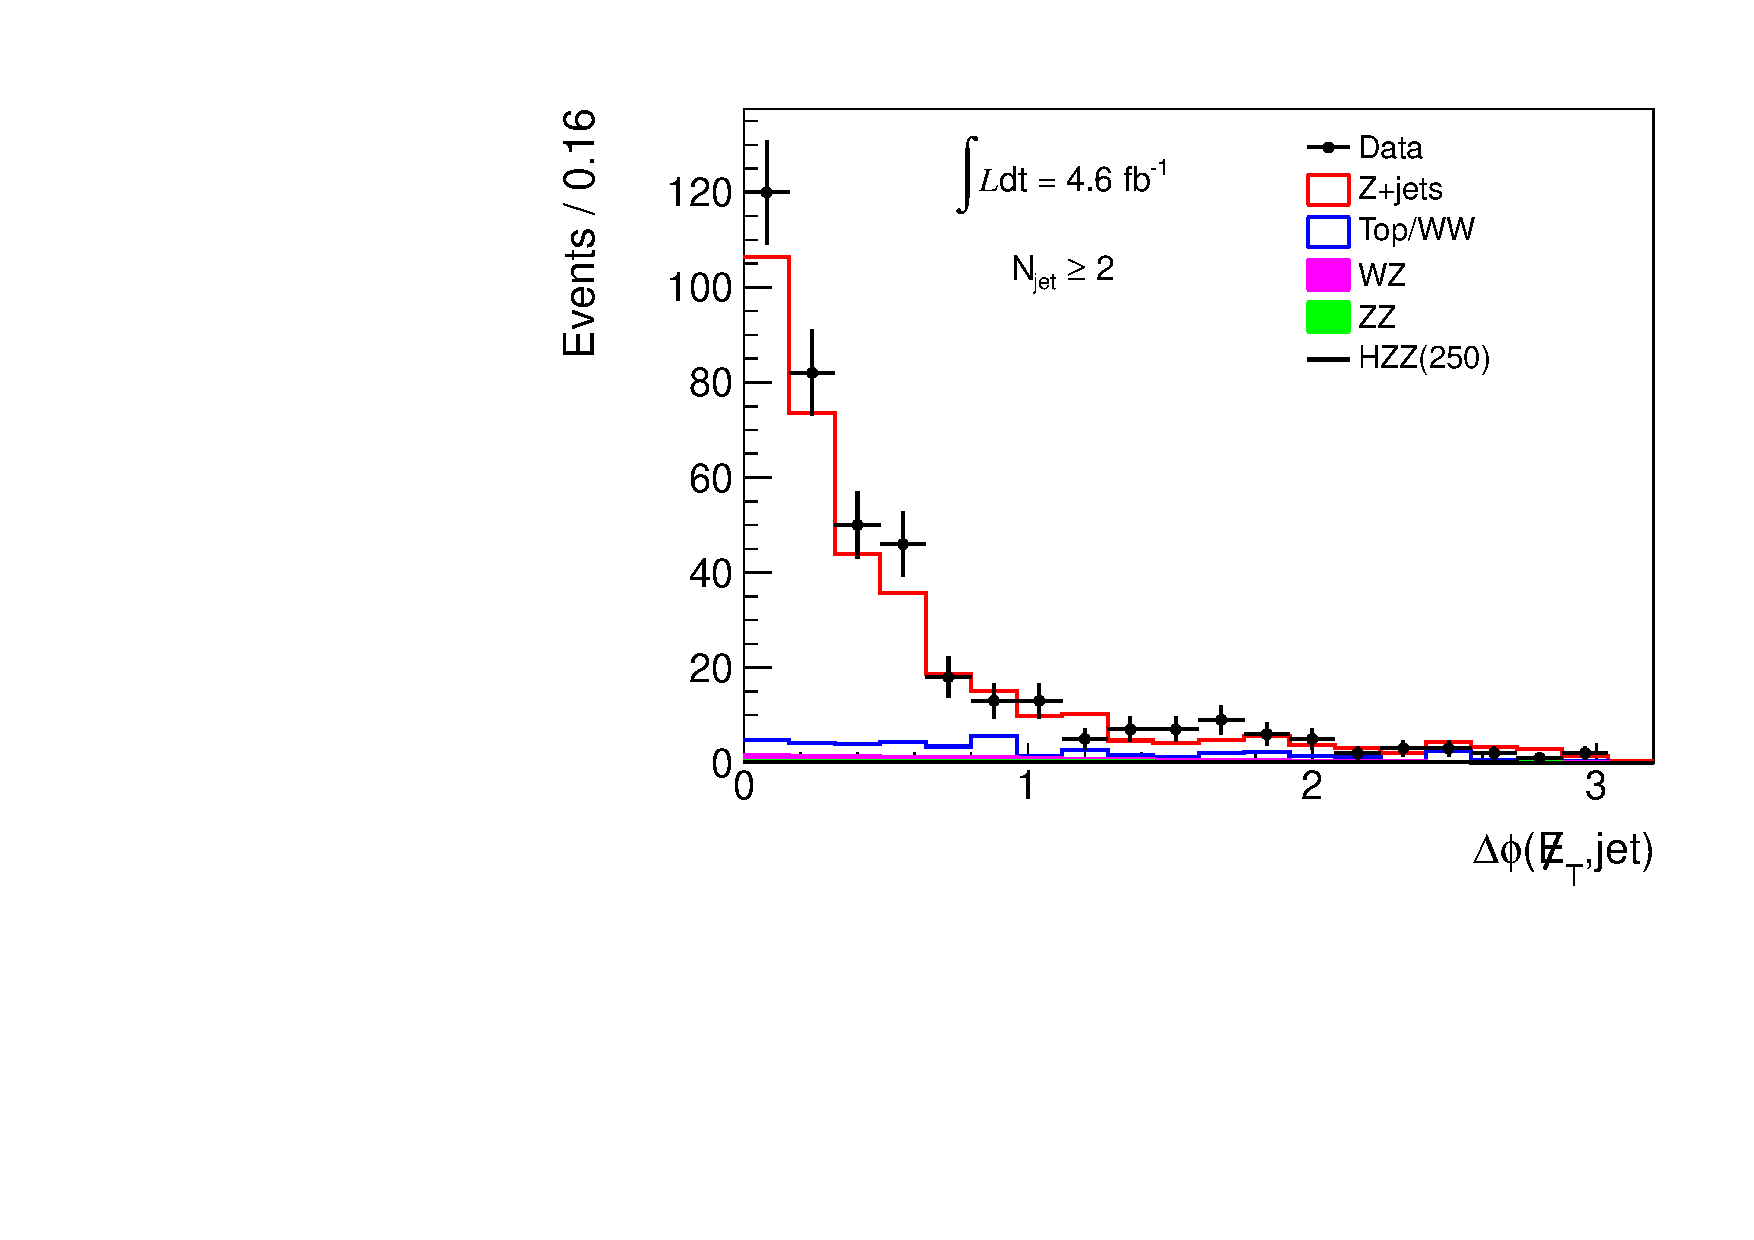
\includegraphics[width=.3\textwidth]{figures/presel_mH250_ee_dphijetmet_2j.pdf}}
\caption{Azimuthal angle separation between \met and the closest jet in the electron channel after the $\ZZ$ preselection observed in data corresponding 
to $2.1$~\ifb data in the Inclusive~\subref{subfig:dphijetmet_mm_incl}, 1-Jet~\subref{subfig:dphijetmet_mm_1j} and 
2-Jet~\subref{subfig:dphijetmet_mm_2j} bins, compared to the expected from simulation for signal and background. The MC backgrounds are scaled as appropriate and 
the photon+jets estimate of the Z+jets background is added to the stack.}
\label{fig:dphijetmet_zzpresel_ee}
\end{center}
\end{figure}
%%%%%%%%

\clearpage

\subsection{Yields after the $\hzz$ selection in cut-based analysis}

The Higgs boson mass dependent signal selections in the cut-based analysis 
are described in Section~\ref{sec:anal_cutbased}. In this section we summarise 
the results obtained all jet final states. 
Tables~\ref{tab:yield_cutbased_ee}-\ref{tab:yield_cutbased_mm} show the signal %equivalent data yields
and background expectations in ee and $\mu\mu$ final states respectively. 
As the signal region is not yet open, we tabulated the expected cross section ratio limits as a function 
of the Higgs mass, together with the 1/2-$\sigma$ uncertainty bands in Table~\ref{tab:limits_cutbased_2fb}.


%%%%%%%%%%%%%%%%%%%%%%%%%
\begin{table}
{\footnotesize
\begin{center}
 \begin{tabular}{l c c c c c c c c }
 \hline
 process & qqH & ggH & ZZ & WZ & WWTop & Zjets & $\sum$Bkg & Data \\
 \hline
250 & $0.5\pm0.1$ & $4.6\pm0.7$ & $9.8\pm1.0$ & $5.6\pm0.7$ & $11.8\pm0.0$ & $7.0\pm2.0$ & $34.3\pm2.3$ & 36 \\
300 & $0.5\pm0.0$ & $4.2\pm0.7$ & $6.0\pm0.6$ & $3.0\pm0.4$ & $3.5\pm0.0$ & $2.0\pm0.6$ & $14.6\pm0.9$ & 18 \\
350 & $0.4\pm0.0$ & $4.4\pm0.7$ & $4.3\pm0.4$ & $1.7\pm0.2$ & $0.5\pm0.0$ & $1.2\pm0.4$ & $7.7\pm0.6$ & 10 \\
400 & $0.3\pm0.0$ & $3.8\pm0.6$ & $3.3\pm0.3$ & $1.2\pm0.2$ & $0.0\pm0.0$ & $1.2\pm0.4$ & $5.7\pm0.5$ & 5 \\
500 & $0.2\pm0.0$ & $1.7\pm0.3$ & $2.0\pm0.2$ & $0.7\pm0.1$ & $0.0\pm0.0$ & $0.8\pm0.3$ & $3.5\pm0.3$ & 3 \\
600 & $0.1\pm0.0$ & $0.6\pm0.1$ & $1.1\pm0.1$ & $0.3\pm0.0$ & $0.0\pm0.0$ & $0.5\pm0.2$ & $2.0\pm0.2$ & 0 \\
\hline
\end{tabular}
\end{center}
}
\caption{Expected number of signal and background events for an 
  integrated luminosity of \intlumi after applying the higgs selections in the cut-based analysis in the ee final state. 
  Only Monte Carlo statistical uncertainties are included. }
\label{tab:yield_cutbased_ee}
%\end{table}
%\begin{table}
{\footnotesize
 \begin{center}
 \begin{tabular}{l c c c c c c c c }
 \hline
 process & qqH & ggH & ZZ & WZ & WWTop & Zjets & $\sum$Bkg & Data \\
 \hline
250 & $0.7\pm0.1$ & $6.3\pm0.9$ & $13.9\pm1.2$ & $7.7\pm0.8$ & $15.9\pm0.0$ & $9.9\pm2.7$ & $47.4\pm3.1$ & 48 \\
300 & $0.6\pm0.0$ & $5.7\pm0.8$ & $8.6\pm0.7$ & $3.9\pm0.4$ & $4.8\pm0.0$ & $3.9\pm1.0$ & $21.2\pm1.3$ & 16 \\
350 & $0.5\pm0.0$ & $5.8\pm0.9$ & $5.8\pm0.5$ & $2.4\pm0.3$ & $0.6\pm0.0$ & $2.1\pm0.6$ & $10.8\pm0.8$ & 4 \\
400 & $0.4\pm0.0$ & $5.1\pm0.7$ & $4.6\pm0.4$ & $1.7\pm0.2$ & $0.0\pm0.0$ & $1.6\pm0.5$ & $7.9\pm0.7$ & 7 \\
500 & $0.2\pm0.0$ & $2.2\pm0.3$ & $2.9\pm0.3$ & $0.8\pm0.1$ & $0.0\pm0.0$ & $1.0\pm0.3$ & $4.7\pm0.4$ & 6 \\
600 & $0.1\pm0.0$ & $0.8\pm0.1$ & $1.6\pm0.1$ & $0.4\pm0.0$ & $0.0\pm0.0$ & $0.7\pm0.3$ & $2.6\pm0.3$ & 2 \\
\hline
\end{tabular}
\end{center}
}
\caption{Expected number of signal and background events for an 
  integrated luminosity of \intlumi after applying the higgs selections in the cut-based analysis in the $\mu\mu$ final state. 
  Only Monte Carlo statistical uncertainties are included. }
\label{tab:yield_cutbased_mm}
\end{table}
%%%%%%%%%%%%%%%%%%%%%%%%%

\begin{table}
\begin{center}
\begin{tabular}{ccccc}
\hline
Mass & Median Expected & [-$\sigma$, +$\sigma$] & [-2$\sigma$, +2$\sigma$]\\\hline
250 & 2.10 & [1.46, 3.03] & [1.07, 4.19] \\
300 & 1.49 & [1.04, 2.14] & [0.77, 3.00] \\
350 & 1.04 & [0.75, 1.54] & [0.56, 2.18] \\
400 & 1.03 & [0.77, 1.55] & [0.56, 2.17] \\
500 & 1.93 & [1.38, 2.91] & [1.09, 4.07] \\
600 & 3.93 & [2.90, 5.88] & [2.17, 8.87] \\
\hline
\end{tabular}
\end{center}
\caption{The median expected cross section ratio limits as a function 
of the Higgs mass, together with the 1/2-$\sigma$ uncertainty bands obtained in the cut-and-count analysis, corresponding to 
an integrated luminosity of \intlumi}
\label{tab:limits_cutbased_2fb}
\end{table}

\subsection{Results in shape analysis} 

The Higgs boson mass dependent signal selections are described in Section~\ref{sec:signal_selection}. 
In this section we summarise the results obtained all jet final states. 
Tables~\ref{tab:yield_shapebased_ee}-\ref{tab:yield_shapebased_mm} show the signal and 
equivalent data yields and background expectations in ee and $\mu\mu$ final states respectively. 
As the signal region is not yet open, we tabulated the expected cross section ratio limits as a function 
of the Higgs mass, together with the 1/2-$\sigma$ uncertainty bands in Table~\ref{tab:limits_mtshape_2fb}. 
The expected limits obtained in shape analysis based on $m_T$ improves the sensitivity upto 10\%, 
considering all the uncertainties on the shape variations. 


%%%%%%%%%%%%%%%%%%%%%%%%%
\begin{table}
{\footnotesize
 \begin{center}
 \begin{tabular}{l | c c | c c c c c c | c}
 \hline
 process & qqH & ggH & ZZ & WZ & WW & Top & Zjets & $\sum$Bkg  & Data\\
 \hline
250 & $0.5\pm0.0$ & $4.2\pm0.7$ & $11.3\pm1.1$ & $6.2\pm0.7$ & $4.6\pm0.7$ & $6.2\pm0.9$ & $6.0\pm1.7$ & $34.3\pm2.5$ & 35 \\
300 & $0.5\pm0.1$ & $4.8\pm0.8$ & $9.0\pm0.9$ & $4.2\pm0.5$ & $2.1\pm0.4$ & $3.8\pm0.8$ & $3.1\pm0.9$ & $22.2\pm1.6$ & 26 \\
350 & $0.5\pm0.1$ & $5.6\pm0.9$ & $10.3\pm1.0$ & $4.7\pm0.6$ & $2.1\pm0.4$ & $3.8\pm0.8$ & $3.4\pm0.9$ & $24.4\pm1.7$ & 28 \\
400 & $0.3\pm0.0$ & $4.7\pm0.9$ & $11.0\pm1.1$ & $4.9\pm0.6$ & $2.1\pm0.4$ & $3.8\pm0.8$ & $3.6\pm1.0$ & $25.5\pm1.8$ & 30 \\
500 & $0.2\pm0.0$ & $2.2\pm0.5$ & $11.8\pm1.2$ & $5.1\pm0.6$ & $2.1\pm0.4$ & $3.8\pm0.8$ & $3.9\pm1.0$ & $26.7\pm1.9$ & 30 \\
600 & $0.1\pm0.0$ & $0.9\pm0.3$ & $12.0\pm1.2$ & $5.1\pm0.6$ & $2.1\pm0.4$ & $3.8\pm0.8$ & $3.9\pm1.0$ & $27.0\pm1.9$ & 30 \\
\hline
\end{tabular}
\end{center}
}
\caption{Expected number of signal and background events for an 
  integrated luminosity of \intlumi after applying the higgs selections in the shape-based analysis in the ee final state. 
  Only Monte Carlo statistical uncertainties are included. }
\label{tab:yield_shapebased_ee}
%\end{table}
%\begin{table}
{\footnotesize
 \begin{center}
 \begin{tabular}{l | c c |  c c c c c c | c }
 \hline
 process & qqH & ggH & ZZ & WZ & WW & Top & Zjets  & $\sum$Bkg & Data \\
 \hline
250 & $0.6\pm0.1$ & $5.7\pm0.9$ & $16.0\pm1.4$ & $8.3\pm0.9$ & $6.1\pm0.9$ & $8.9\pm1.3$ & $9.5\pm2.6$ & $48.9\pm3.5$ & 43 \\
300 & $0.7\pm0.1$ & $6.5\pm1.0$ & $12.8\pm1.1$ & $5.6\pm0.6$ & $3.2\pm0.6$ & $5.1\pm1.0$ & $5.6\pm1.5$ & $32.3\pm2.3$ & 24 \\
350 & $0.6\pm0.1$ & $7.6\pm1.2$ & $14.6\pm1.3$ & $6.2\pm0.7$ & $3.2\pm0.6$ & $5.2\pm1.0$ & $5.9\pm1.6$ & $35.0\pm2.4$ & 26 \\
400 & $0.5\pm0.1$ & $6.5\pm1.1$ & $15.7\pm1.3$ & $6.5\pm0.7$ & $3.2\pm0.6$ & $5.2\pm1.0$ & $6.1\pm1.6$ & $36.6\pm2.5$ & 29 \\
500 & $0.3\pm0.1$ & $2.8\pm0.7$ & $16.8\pm1.4$ & $6.7\pm0.7$ & $3.2\pm0.6$ & $5.2\pm1.0$ & $6.5\pm1.7$ & $38.3\pm2.7$ & 31 \\
600 & $0.2\pm0.1$ & $1.1\pm0.4$ & $17.1\pm1.5$ & $6.7\pm0.7$ & $3.2\pm0.6$ & $5.2\pm1.0$ & $6.5\pm1.7$ & $38.7\pm2.7$ & 31 \\
\hline
\end{tabular}
\end{center}
}
\caption{Expected number of signal and background events for an 
  integrated luminosity of \intlumi after applying the higgs selections in the shape-based analysis in the $\mu\mu$ final state. 
  Only Monte Carlo statistical uncertainties are included. }
\label{tab:yield_shapebased_mm}
\end{table}
%%%%%%%%%%%%%%%%%%%%%%%%%

\begin{table}
\begin{center}
{\normalsize
\begin{tabular}{|l|c|c|c|c|c|c|}
\hline
      &  \multicolumn{3}{c|}{ without shape uncertainty} &\multicolumn{3}{c|}{ with shape uncertainty} \\
\hline
Mass  &  Median      &     68\% C.L. band &  95\% C.L. band &  Median	   &	 68\% C.L. band &  95\% C.L. band\\
      &  Expected    &                    &                 &  Expected    &			&		 \\
\hline
250 & 1.87 & [1.32, 2.66] & [0.97, 3.67] & 1.92 & [1.36, 2.75] & [1.01, 3.84] \\
300 & 1.29 & [0.91, 1.83] & [0.68, 2.54] & 1.32 & [0.94, 1.90] & [0.70, 2.63] \\
350 & 0.95 & [0.69, 1.36] & [0.51, 1.88] & 0.97 & [0.70, 1.40] & [0.52, 1.96] \\
400 & 0.99 & [0.71, 1.42] & [0.53, 1.97] & 1.00 & [0.72, 1.45] & [0.54, 2.03] \\
500 & 1.87 & [1.35, 2.68] & [1.03, 3.75] & 1.91 & [1.37, 2.76] & [1.05, 3.91] \\
600 & 4.31 & [3.09, 6.19] & [2.42, 8.83] & 4.41 & [3.15, 6.40] & [2.42, 9.09] \\
\hline
\end{tabular}
}
\end{center}
\caption{The median expected cross section ratio limits as a function 
of the Higgs mass, together with the 1/2-$\sigma$ uncertainty bands obtained in the shape analysis based on $M_T$, corresponding to 
an integrated luminosity of \intlumi}
\label{tab:limits_mtshape_2fb}
\end{table}
